% Options for packages loaded elsewhere
\PassOptionsToPackage{unicode}{hyperref}
\PassOptionsToPackage{hyphens}{url}
\PassOptionsToPackage{dvipsnames,svgnames,x11names}{xcolor}
\PassOptionsToPackage{space}{xeCJK}
\documentclass[
  12pt,
  a4paper]{ctexbook}
\usepackage{xcolor}
\usepackage[top=2.5cm,bottom=2.5cm,left=3cm,right=2.6cm]{geometry}
\usepackage{amsmath,amssymb}
\setcounter{secnumdepth}{5}
\usepackage{iftex}
\ifPDFTeX
  \usepackage[T1]{fontenc}
  \usepackage[utf8]{inputenc}
  \usepackage{textcomp} % provide euro and other symbols
\else % if luatex or xetex
  \usepackage{unicode-math} % this also loads fontspec
  \defaultfontfeatures{Scale=MatchLowercase}
  \defaultfontfeatures[\rmfamily]{Ligatures=TeX,Scale=1}
\fi
\usepackage{lmodern}
\ifPDFTeX\else
  % xetex/luatex font selection
  \ifXeTeX
    \usepackage{xeCJK}
    \setCJKmainfont[]{Songti SC}
    \setCJKsansfont[]{Hiragino Sans GB}
  \fi
  \ifLuaTeX
    \usepackage[]{luatexja-fontspec}
    \setmainjfont[]{Songti SC}
  \fi
\fi
% Use upquote if available, for straight quotes in verbatim environments
\IfFileExists{upquote.sty}{\usepackage{upquote}}{}
\IfFileExists{microtype.sty}{% use microtype if available
  \usepackage[]{microtype}
  \UseMicrotypeSet[protrusion]{basicmath} % disable protrusion for tt fonts
}{}
\usepackage{setspace}
\makeatletter
\@ifundefined{KOMAClassName}{% if non-KOMA class
  \IfFileExists{parskip.sty}{%
    \usepackage{parskip}
  }{% else
    \setlength{\parindent}{0pt}
    \setlength{\parskip}{6pt plus 2pt minus 1pt}}
}{% if KOMA class
  \KOMAoptions{parskip=half}}
\makeatother
\usepackage{longtable,booktabs,array}
\newcounter{none} % for unnumbered tables
\usepackage{calc} % for calculating minipage widths
% Correct order of tables after \paragraph or \subparagraph
\usepackage{etoolbox}
\makeatletter
\patchcmd\longtable{\par}{\if@noskipsec\mbox{}\fi\par}{}{}
\makeatother
% Allow footnotes in longtable head/foot
\IfFileExists{footnotehyper.sty}{\usepackage{footnotehyper}}{\usepackage{footnote}}
\makesavenoteenv{longtable}
\usepackage{graphicx}
\makeatletter
\newsavebox\pandoc@box
\newcommand*\pandocbounded[1]{% scales image to fit in text height/width
  \sbox\pandoc@box{#1}%
  \Gscale@div\@tempa{\textheight}{\dimexpr\ht\pandoc@box+\dp\pandoc@box\relax}%
  \Gscale@div\@tempb{\linewidth}{\wd\pandoc@box}%
  \ifdim\@tempb\p@<\@tempa\p@\let\@tempa\@tempb\fi% select the smaller of both
  \ifdim\@tempa\p@<\p@\scalebox{\@tempa}{\usebox\pandoc@box}%
  \else\usebox{\pandoc@box}%
  \fi%
}
% Set default figure placement to htbp
\def\fps@figure{htbp}
\makeatother
\setlength{\emergencystretch}{3em} % prevent overfull lines
\sloppy
\setlength{\parindent}{2em}
\setlength{\parskip}{0pt}
\providecommand{\tightlist}{%
  \setlength{\itemsep}{0pt}\setlength{\parskip}{0pt}}
\usepackage{bookmark}
\IfFileExists{xurl.sty}{\usepackage{xurl}}{} % add URL line breaks if available
\urlstyle{same}
\hypersetup{
  pdftitle={中学生物理竞赛复赛试题的科学思维要求与教学转化研究},
  pdfauthor={董兴习},
  colorlinks=true,
  linkcolor={black},
  filecolor={Maroon},
  citecolor={Blue},
  urlcolor={blue},
  pdfcreator={LaTeX via pandoc}}

\title{中学生物理竞赛复赛试题的科学思维要求与教学转化研究}
\author{董兴习}
\date{2026年7月}

\begin{document}
\frontmatter
\maketitle

{
\setcounter{tocdepth}{2}
\tableofcontents
}
\setstretch{1.5}
\mainmatter
\chapter*{摘要}\addcontentsline{toc}{chapter}{摘要}\label{ux6458ux8981}

以第35至42届全国中学生物理竞赛复赛试题为对象，分析试题任务在模型建构、科学推理、科学论证和质疑创新四个维度上的认知要求，并提出相应的教学转化建议。以独立小问为分析单位，建立219个分析单元，采用内容分析法形成876条编码记录；在编码框架经专家审阅和研究者复核后，对维度出现、等级构成和维度共现进行描述统计，并结合题干与参考解答开展典型案例分析。结果表明：模型建构、科学推理、科学论证和质疑创新分别出现于203、219、106和84个分析单元；模型建构、科学推理和科学论证在出现单元中均以L1占比最高，质疑创新以L2占比最高；模型建构与科学推理共同出现于203个分析单元，科学论证与质疑创新共同出现于40个分析单元，二者并集为150个分析单元。基于分析结果，提炼出条件---关系链、状态分类---能量关系和近似条件建模三类任务结构，并据此提出任务设计、支架设计和评价建议。本研究从小问级语料、编码证据、描述统计和案例分析之间建立了可追溯的分析路径，可为物理竞赛试题研究与竞赛教学设计提供参考。研究结果描述的是试题及其参考解答呈现的任务认知要求，不直接推断学生实际能力或教学效果。

关键词：物理竞赛；科学思维；试题分析；内容分析；任务认知要求

\chapter*{ABSTRACT}\addcontentsline{toc}{chapter}{ABSTRACT}\label{abstract}

This study examines the cognitive requirements represented in the
second-round papers from the 35th to the 42nd editions of the National
Physics Competition for High School Students in China and develops
corresponding suggestions for instructional translation. Analytically
distinct subquestions were used as units of analysis, yielding 219
analysis units and 876 coding records. Following expert review of the
coding framework and researcher review, descriptive statistics were
produced for dimensional presence, level composition, and co-occurrence,
and representative cases were examined through item and
reference-solution evidence. Model construction, scientific reasoning,
scientific argumentation, and questioning and innovation occurred in
203, 219, 106, and 84 analysis units, respectively. L1 was the most
frequent level among units where model construction, scientific
reasoning, or scientific argumentation occurred, whereas L2 was the most
frequent level for questioning and innovation. Model construction and
scientific reasoning co-occurred in 203 analysis units; scientific
argumentation and questioning and innovation co-occurred in 40 units,
with a union of 150 units. Three task structures were identified:
condition-relation chains, state classification-energy relations, and
modeling with approximation conditions. The study provides an
evidence-linked analytical path from subquestion-level corpus records to
coding, descriptive statistics, and case analysis, offering a reference
for physics competition item research and instructional design. The
findings describe cognitive requirements represented by items and
reference solutions and do not directly indicate students' actual
capabilities or instructional effectiveness.

Keywords: physics competition; scientific thinking; test-item analysis;
content analysis; task cognitive requirements

\chapter{绪论}\label{ux7eeaux8bba}

\section{研究背景与问题提出}\label{ux7814ux7a76ux80ccux666fux4e0eux95eeux9898ux63d0ux51fa}

\subsection{科学思维与竞赛试题分析}\label{ux79d1ux5b66ux601dux7ef4ux4e0eux7adeux8d5bux8bd5ux9898ux5206ux6790}

普通高中物理课程改革将科学思维作为物理学科核心素养的重要组成部分，并将模型建构、科学推理、科学论证、质疑创新列为科学思维的重要表现。\textsuperscript{[1]}
课程标准为本研究选择科学思维维度、界定分析内容提供了理论依据；在此基础上，本文结合复赛试题的题干、参考解答和编码规则开展具体分析。

复赛试题分析不宜只停留在知识点、题型或难度描述，还需要关注试题实际要求解题者完成的认知活动：如何抽象物理模型，如何组织条件链，如何说明边界条件，如何在陌生情境中迁移或修正已有模型。因此，本文从科学思维维度和任务认知结构要求两个层面分析复赛试题。

本文整理第35至42届全国中学生物理竞赛复赛试题与参考答案，以独立小问为基本单位，共形成219个分析单元和876条维度编码记录。每条记录均对应题干触发语和参考解答关键步骤，第四章据此呈现维度分布、等级构成与共现关系。相关统计描述的是试题任务要求，不用于推断学生能力、教学效果或命题趋势。

全国中学生物理竞赛复赛试题具有综合性强、情境多样、推导链条长的特点。一道题目往往同时包含物理对象的抽象、条件与边界的确定、规律关系的组织、数学工具的使用以及结果的解释。若仅从力学、电磁学、光学或近代物理等知识模块分类，能够说明题目涉及的内容范围，却难以揭示解题者在完成任务时需要进行何种思维活动；若只依据题量、分值、公式数量或计算长度判断难度，也容易忽略不同题目在模型设定、推理组织和论证要求上的差异。

以任务结构为中心的分析能够补充这一不足。它不把竞赛题简化为``考查某一知识点''，而是考察题干与参考解答共同要求解题者完成的活动：是否需要从复杂情境中确定研究对象和理想化条件，是否需要将多个规律与条件组织为关系链，是否需要比较不同情形或说明结论的适用范围，是否需要修正假设或构造新的方案。这样的视角既能保持物理内容的具体性，也能把不同题材中的相似思维要求识别出来。

复赛题的教学价值也由此得到更细致的理解。竞赛训练当然需要掌握较高水平的物理知识与数学工具，但训练过程不应只表现为``看懂答案---模仿步骤---完成计算''。当教师能够识别一道题中最关键的条件、模型、推理或论证环节时，就可以设计相应的追问、书面产出和反馈方式，使学生不仅获得结论，也理解结论如何由条件和规律共同支撑。本文正是在这一背景下，尝试将试题分析与教学转化联系起来。

由此，本研究的问题意识可以概括为：复赛试题到底要求学生进行怎样的科学思维活动，如何把这些要求转化为可编码、可复核的分析框架，又如何在不夸大证据的前提下，将试题分析结果转化为竞赛教学中的任务、支架和评价设计。

\section{核心概念与研究边界}\label{ux6838ux5fc3ux6982ux5ff5ux4e0eux7814ux7a76ux8fb9ux754c}

\subsection{核心概念界定}\label{ux6838ux5fc3ux6982ux5ff5ux754cux5b9a}

本研究以模型建构、科学推理、科学论证、质疑创新四个维度组织试题分析。这一维度结构具有课程标准依据，\textsuperscript{[1]}
每个维度均通过编码手册、边界案例和一致性检验落实为可操作的判定规则。

本研究中的``认知要求''指试题及参考解答对解题者提出的任务要求，而不是学生实际达到的能力水平。换言之，论文分析的是``题目要求完成什么样的思维活动''，不是``学生已经具备什么能力''。科学推理和科学思维测评研究也提示，学生能力判断需要测评任务、作答数据和模型检验，不能由试题文本分析直接推出。\textsuperscript{[2, 3]}
没有学生作答、访谈、课堂观察或测评数据时，不能把试题编码结果解释为学生科学思维水平。

本研究中的``SOLO启发等级''只用于描述某一科学思维维度出现时的任务结构复杂性。本文使用``SOLO启发的任务认知结构要求等级''这一表述，不将试题直接等同于学生学习结果等级。

本研究中的``教学转化''指把试题分析发现转化为任务设计、支架设计、评价量规和反馈方式。科学论证教学研究和国际科学实践框架可以为``任务、支架、评价对象''的设计提供参照，\textsuperscript{[4, 5]}
但它不等于教学策略已经有效。当前项目尚无真实教师访谈、问卷、课堂记录、学生作品或前后测数据，因此第一章只能把教学转化写作研究目标和后续任务，不能提前写成教学效果结论。

\section{国内外研究现状}\label{ux56fdux5185ux5916ux7814ux7a76ux73b0ux72b6}

\subsection{研究视角与文献基础}\label{ux7814ux7a76ux89c6ux89d2ux4e0eux6587ux732eux57faux7840}

本研究的文献综述拟围绕四组材料展开。第一组是课程标准和科学思维理论，用于说明为什么以模型建构、科学推理、科学论证、质疑创新组织分析。第二组是SOLO理论及任务分析相关研究，用于说明为什么本研究只能把SOLO作为任务认知结构等级的启发来源。第三组是物理竞赛试题研究，用于比较既有研究在样本范围、分析单位和分析视角上的处理方式。第四组是内容分析、评分者一致性和教学转化研究，用于支撑编码流程、质量检验和结果转化；其中编码者一致性报告的边界已有一个方法来源可作有限支持。\textsuperscript{[6]}

现有研究分别提供了科学思维要素、任务结构解释、内容分析程序和教学设计参照。\textsuperscript{[1, 2, 3, 4, 5, 6]}
这些研究提示，有必要从科学思维维度和任务结构角度补充复赛小问级证据；本文据此提出研究问题，而不把这一判断表述为对既有研究的穷尽性否定。

因此，本章以研究问题所需的文献脉络为主，第二章再围绕科学思维、SOLO启发的任务结构、内容分析与教学转化展开系统讨论，并将每类文献放在其能够支撑的论证位置上。

\subsection{国内物理竞赛试题研究}\label{ux56fdux5185ux7269ux7406ux7adeux8d5bux8bd5ux9898ux7814ux7a76}

国内关于中学生物理竞赛试题的研究已经形成若干较有代表性的路径。第一类研究以典型题为对象，从核心素养或科学思维角度分析题目情境、物理过程与解答要求。此类研究能够较细致地揭示一道或若干道题目中蕴含的物理思想，但样本数量较少，结论主要适用于所选案例。第二类研究以若干届试卷为样本，围绕题型、知识板块、分值、题量或考查内容进行统计，能够展示试卷结构的总体特征，却较少进入小问层面的任务结构。第三类研究引入SOLO分类或综合难度模型，尝试用明确的分类规则分析复赛理论题，为竞赛试题的系统研究提供了重要参照。\textsuperscript{[13, 15, 16, 17]}

预赛研究通常重视题型、知识分布和典型题的素养表现。凌国亮等以预赛典型题及其解答过程讨论数理核心素养，强调从题目条件、物理规律和推导过程理解考查要求；另有研究以多届预赛卷为材料，对题型、分值、知识板块和考查内容进行量化描述。这些研究说明，竞赛试题分析既可以从具体题目切入，也可以从多届试卷结构切入。由于预赛与复赛在任务开放度、计算深度和题目组织方式上存在差异，预赛研究的统计口径不能直接替代复赛小问级分析，但其关于语料范围、分析变量和规则公开的处理具有方法启示。\textsuperscript{[15, 16]}

复赛研究更接近本研究的对象。龚枭以第26至35届复赛理论题为材料，使用SOLO分类理论组织试题分析；张豇萌以第34至38届复赛理论题为样本，依据综合难度模型对试题进行统计。两项研究共同表明，复赛理论题可以进行跨届、系统的文本研究，也需要说明样本范围、分析单位和赋值规则。二者的研究重点分别在整题SOLO分类和综合难度构成，而本文将独立小问作为基本单位，分别记录模型建构、科学推理、科学论证和质疑创新的出现及其任务结构要求。这样的差异并非否定既有研究，而是将关注点从``题目总体属于何种类型或难度''转向``题目要求解题者完成哪些思维活动''。\textsuperscript{[13, 17]}

唐路的研究还将复赛、决赛题目统计与成绩资料、案例分析并置，提示竞赛题研究中存在题目文本、试题统计和参赛者表现等多种证据来源。不同证据回答的问题不同：题目与参考解答能够说明任务要求，成绩资料能够呈现特定样本的作答表现，访谈或课堂资料才能进一步讨论学习过程。本文聚焦前一类证据，因此不将试题编码结果延伸为地区成绩、学生能力或教学效果的结论。\textsuperscript{[14]}

\subsection{本研究的切入点}\label{ux672cux7814ux7a76ux7684ux5207ux5165ux70b9}

综合已有研究可以发现，竞赛试题研究正在从知识点归类和试卷结构统计走向更细致的任务分析，但在复赛语料中，仍有必要进一步说明分析单位、判定依据和任务结构之间的关系。以整题为单位时，同一题中不同小问可能被合并为同一种难度或层次；以分值或公式数量作为主要指标时，模型简化、条件组织、论证说明和方案比较等差异也容易被遮蔽。小问级分析能够保留这些差异，使不同维度在同一题内的组合关系得到呈现。

从研究对象、分析单位与结果解释三个方面比较，现有路径各有适用范围。以典型题为中心的研究有利于深入说明一个物理问题中概念、规律和情境之间的联系，但其结论通常不宜外推到整套试题；以整卷或整题为单位的统计便于描绘题型、知识模块与分值结构，却容易把同一大题内部由基础推演到条件讨论的层次变化压缩为一个标签；以综合难度模型为基础的研究能够提供多指标比较，却不能自动回答某一小问究竟要求解题者进行建模、论证还是方案调整。本文并不试图以一种分类替代上述研究，而是把独立小问作为观察窗口：统计结果首先回答``哪些任务要求出现''，随后再回到题干和解答说明``这些要求如何在物理求解中发生''。

这一选择也影响论文对``差异''的理解。若某一知识模块中科学论证记录较多，本文不会把它解释为该模块天然更高级，而会进一步追问：该模块的题目是否较多出现比较、极限、近似或适用范围说明；若某一届质疑创新记录较少，也不能据此判断命题质量高低，而应考察该届题目是否更多在已给模型中展开推演。换言之，统计表提供的是检索和比较的入口，物理任务的具体组织才是解释的落点。这样的处理既保留跨届语料的整体视野，也避免让百分比脱离题目本身。

因此，本文的研究定位包括三个方面：其一，以第35至42届复赛试题的独立小问为分析单位，形成跨届而颗粒度较细的语料；其二，以科学思维四维度和SOLO启发的任务结构等级构成两层分析框架，避免将知识内容、难度和思维要求混为一谈；其三，在描述性统计之外回到题干与参考解答，选取具有代表性的任务结构案例，提出面向竞赛教学的任务、支架和评价建议。上述定位使本文既保持竞赛试题研究的系统性，也保留对具体物理任务的解释力。

本文所说的教学转化也因此不是把统计比例逐条改写成教学口号。真正能够进入教学设计的是统计背后反复出现的任务结构：例如，若一个小问的关键在于把限制条件引入关系链，教学中就应让学生呈现条件如何进入推导；若一个小问的关键在于状态分类，教学中就应让学生说明分类依据与比较对象；若一个小问依赖近似假设，教学中就应让学生解释忽略什么、保留什么以及结论适用到何处。这样的转化路径把研究结果、学生可见产出和教师反馈连接起来，同时不把尚未收集的学生表现预先写入研究结论。

\section{研究问题}\label{ux7814ux7a76ux95eeux9898}

\subsection{研究问题设计}\label{ux7814ux7a76ux95eeux9898ux8bbeux8ba1}

结合研究语料、分析方法和证据范围，本研究回答以下问题：

\begin{enumerate}
\def\labelenumi{\arabic{enumi}.}
\tightlist
\item
  如何构建适用于全国中学生物理竞赛复赛试题的科学思维认知要求分析框架？
\item
  第35至42届复赛试题在模型建构、科学推理、科学论证和质疑创新四个维度上呈现出怎样的任务要求？
\item
  这些试题在认知结构要求等级、维度组合和典型题设机制上有哪些特征？
\item
  不同知识模块、情境类型、表征形式和数学工具下，试题认知要求是否呈现可描述的差异？
\item
  如何将试题分析结果转化为竞赛教学中的任务、支架和评价设计？
\end{enumerate}

上述问题中，第2至第4个问题基于编码表作描述性回答，不据此推断学生能力、命题长期趋势或因果关系。第5个问题着重回答``如何设计''，不以试题分析代替教学效果检验。

\subsection{研究问题之间的逻辑关系}\label{ux7814ux7a76ux95eeux9898ux4e4bux95f4ux7684ux903bux8f91ux5173ux7cfb}

五个研究问题不是彼此孤立的。第一个问题解决``用什么语言分析试题''的问题：只有先明确四个维度分别观察什么、等级如何理解，后续的统计才有共同口径。第二个问题回答全样本中各类任务要求的基本分布，第三个问题进一步考察这些要求在等级和组合上的结构特征，第四个问题把这种结构放回知识模块、届次和题面材料条件中寻找可供阅读的线索。第五个问题则把统计和案例中已经识别出的任务结构，转化为可安排、可观察的教学活动。

这种由框架到分布、由分布到案例、再由案例到教学设计的顺序，能够避免两种常见的跳跃。其一，不能只凭某一题``综合''或``新颖''就断言它具有某一种科学思维要求；任务的判定仍需回到题干和参考解答。其二，不能把总体百分比直接翻译成教学结论；例如，某一维度出现较多，只说明相应任务要求在当前语料中较常见，还需要结合其具体表现形式设计学习任务。研究问题之间的衔接，正是为了使结论既保留总体视野，也不脱离物理问题本身。

\subsection{各研究问题的回答依据}\label{ux5404ux7814ux7a76ux95eeux9898ux7684ux56deux7b54ux4f9dux636e}

第一个问题主要依据课程标准中的科学思维要素、SOLO启发的任务结构理解、编码手册及边界案例回答。其重点不是为四个维度赋予抽象定义，而是说明何种题干要求和解答步骤可以作为判定依据。第二至第四个问题主要依据219个分析单元的编码记录、元数据索引和描述统计表回答，其中统计数字必须与题干和解答证据相互对应。第五个问题以典型案例中可见的条件识别、模型组织、关系推演、比较说明和边界核对为依据，形成任务、支架和评价产出的设计建议。

不同问题所依托的材料不同，结论强度也应有所区别。全样本编码表可以支持``某种任务要求在本语料中出现多少次''的描述；典型案例可以支持``这种要求在某一物理任务中如何实现''的解释；教学设计材料可以支持``可据此设计何种学习产出''的建议。本文据此将试题任务要求、学生实际表现和教学效果分开处理，使每一部分的论证都有清楚的材料来源。

\section{研究内容、方法和技术路线}\label{ux7814ux7a76ux5185ux5bb9ux65b9ux6cd5ux548cux6280ux672fux8defux7ebf}

\subsection{研究内容与技术路线}\label{ux7814ux7a76ux5185ux5bb9ux4e0eux6280ux672fux8defux7ebf}

本研究采用``复赛试题内容分析---典型机制解释---教学转化设计''的路线。论文以第35至42届复赛试题为语料，将典型试题机制分析与基于任务结构的教学设计建议相衔接；教学转化部分限于设计建议，不作教学效果验证。

研究内容包括五部分。第一，建立复赛试题小问级语料库，记录题号、小问、页码、知识模块、情境、表征和数学工具等信息。第二，基于课程标准、SOLO启发等级和内容分析方法，形成科学思维维度与任务认知结构等级的编码框架。第三，开展双人编码、一致性分析和分歧裁决，形成用于统计的编码表；一致性报告按变量说明样本、指标选择和分歧处理。\textsuperscript{[6]}
第四，生成维度分布、等级分布、共现关系和典型机制的描述性分析。第五，将分析结果转化为竞赛教学中的任务设计、支架设计和评价建议。\textsuperscript{[4, 5]}

技术路线如下：

\noindent\pandocbounded{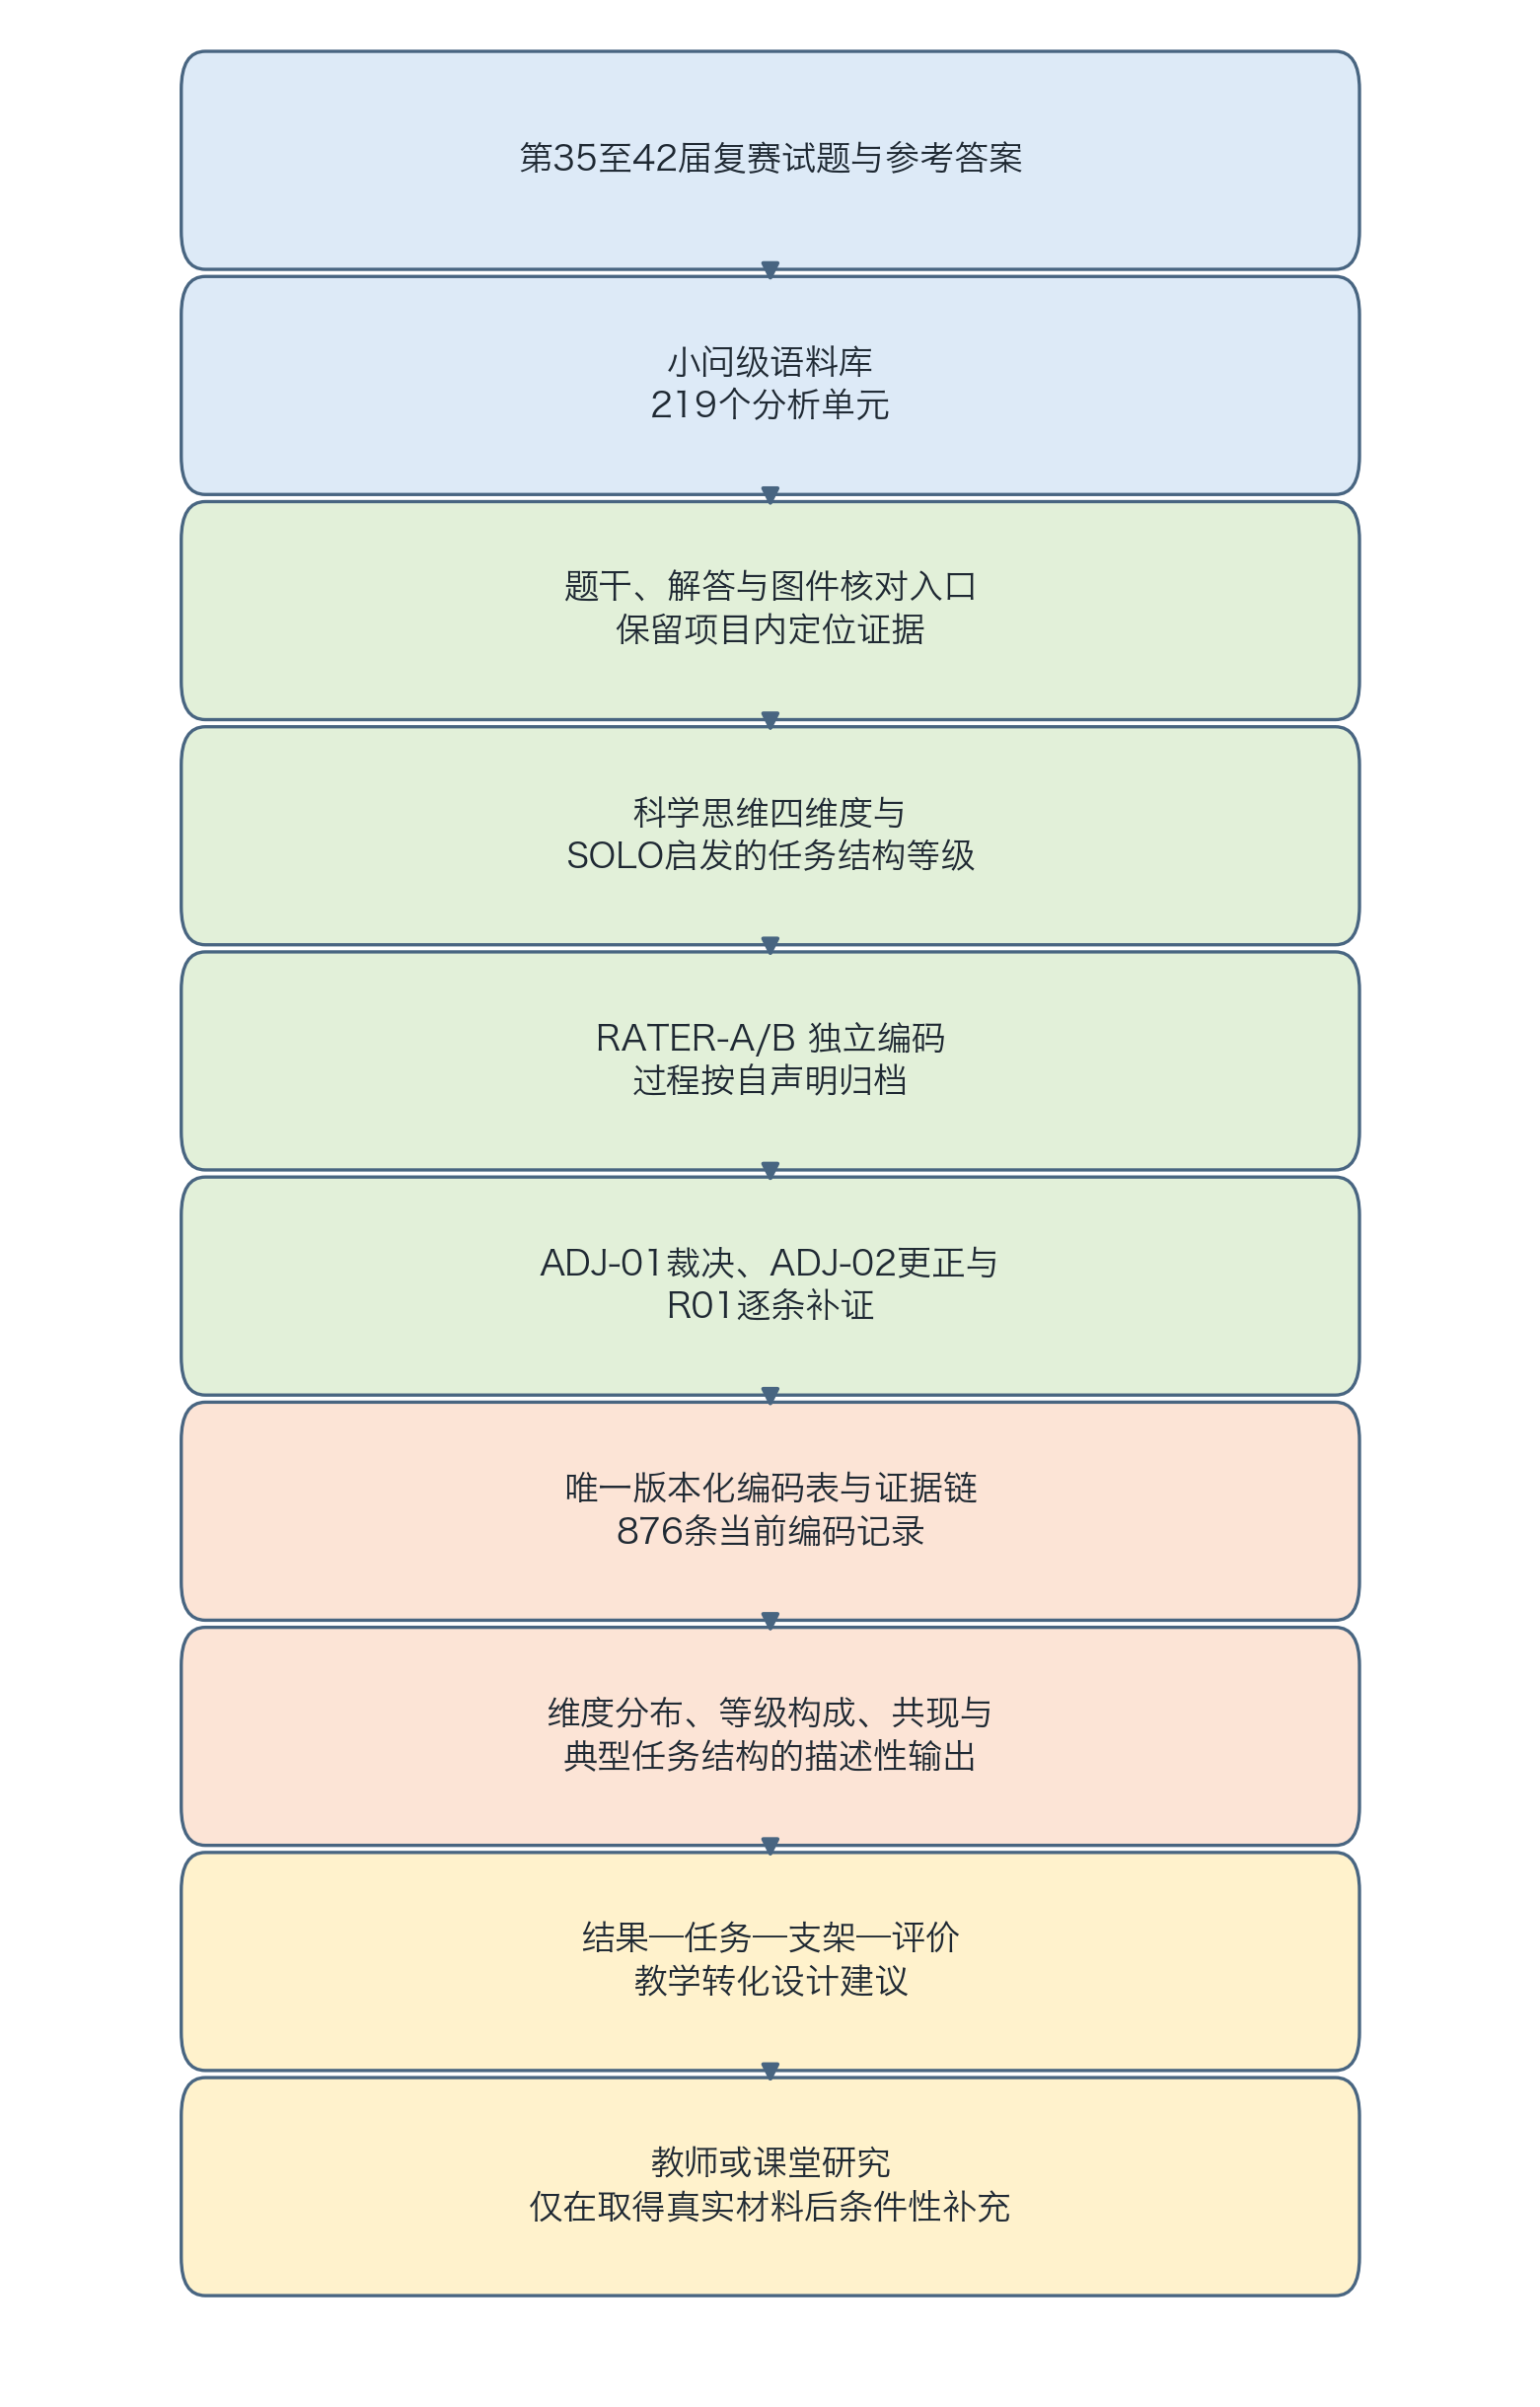
\includegraphics[keepaspectratio]{08_manuscript/figures/figure_1_1_r01_technical_route_v1.png}}

图1-1 试题分析与教学转化技术路线。

研究按照``语料整理---框架建构---编码统计---案例解释---教学设计''的顺序展开。教学转化以试题任务结构为依据，形成可用于选题、评讲和评价的设计建议；其效果仍需由真实课堂研究进一步检验。

从研究实施的角度看，语料建立、框架编码和教学转化承担着不同作用。语料建立确保每一个统计单元都有明确的题面和答案定位；框架编码将分散的物理任务转化为可以比较的维度与等级记录；描述统计用于呈现整体结构；案例分析负责解释统计背后的任务机制；教学转化则把这些机制重新组织为课堂中可提交、可讨论的学习产出。各环节之间以题号、小问和证据定位连接，而不是以研究者的主观印象连接。

在这一技术路线中，参考解答的作用也需要明确。参考解答不是学生作答的替代物，而是判断一道题完成任务所需的典型物理关系、条件处理和结果说明的重要参照。当题干只提出目标而未显露完整推演时，解答可以帮助识别该目标所依赖的关键步骤；当题干已经给出明确模型时，解答又可以显示哪些关系只是常规推进，哪些环节涉及分情形、近似、比较或修正。因而，题干与解答需要同时进入分析，但二者分别承担任务提出与求解结构说明的功能。

教学转化并不是在统计完成后附加几条一般性建议，而是从案例中抽取可操作的学习环节。例如，面对条件较多的任务，可先要求学生完成条件表与关系图；面对状态分类任务，可要求学生说明分类依据并列出相应表达式；面对近似条件任务，可要求学生解释忽略项改变了模型的什么部分。由此形成的任务设计与第四章的统计、第五章的案例相互衔接，使``试题分析''能够真正转化为竞赛教学中的材料选择和追问设计。

\section{研究价值与创新}\label{ux7814ux7a76ux4ef7ux503cux4e0eux521bux65b0}

\subsection{理论价值与实践意义}\label{ux7406ux8bbaux4ef7ux503cux4e0eux5b9eux8df5ux610fux4e49}

本文的价值主要体现在三个方面。第一，在研究对象上，形成第35至42届复赛试题的小问级语料与元数据，为复赛试题研究提供更细的分析单位。第二，在方法上，将科学思维维度与任务认知结构要求分开编码，减少把知识点、计算难度和思维要求混为一谈的风险。第三，在实践上，将试题分析结果转化为竞赛教学中的任务、支架和评价设计，使教学建议回到试题证据和可观察的学习产出。

这些价值应当由实际研究产出支撑，而不宜提前宣称已经实现。本文已形成版本化编码表、一致性与裁决档案、逐条证据链及描述性输出；教学转化部分则以完整案例设计为基础，不对课堂成效作出未经课堂材料支持的结论。

\subsection{理论价值}\label{ux7406ux8bbaux4ef7ux503c}

在理论层面，本文将科学思维作为分析竞赛试题任务要求的视角，而不是将其直接等同于学生的稳定能力。这样的处理有助于把课程标准中的科学思维要素转化为可讨论的题目结构：模型建构关注系统、条件与假设，科学推理关注由条件到结论的关系组织，科学论证关注理由与结论之间的支撑，质疑创新关注假设、方案和模型的调整。四个维度共同构成理解复赛题``要求解题者做什么''的分析语言。

本文还将SOLO理论作为描述任务认知结构的启发资源，与科学思维维度形成两层框架。前一层回答任务包含哪一类科学思维要求，后一层回答该要求需要处理单一要素、并列要素、关联要素还是迁移拓展。两层框架避免将``知识综合''\,``计算量大''或``题目陌生''直接视为高层次思维，也避免以一个总分覆盖不同性质的任务要求。这一处理为竞赛题、考试题及其他物理文本的任务分析提供了可迁移的思路。

\subsection{方法价值}\label{ux65b9ux6cd5ux4ef7ux503c}

在方法层面，本文以小问而非整道大题作为主要分析单位。复赛题往往在同一大题中设置多个目标量、不同条件或连续递进的任务，整题分析容易掩盖其中的结构差异。小问级索引将届次、题号、页码、知识模块、情境、表征、数学工具和答案结构与编码记录连接起来，使总体统计能够回到具体题目，也使案例选择不只依赖研究者的印象。

本文还将维度存在性、结构等级、题干证据与解答证据分别记录。对于内容分析研究而言，统计表的可靠性不只取决于最终比例，也取决于每一个判断能否被回查。通过保留题干触发语、解答关键步骤和相邻等级排除理由，研究者能够说明某一小问为何被判为某一维度或等级；当规则修订时，也能识别哪些统计、图表和案例需要同步更新。这样的记录方式为后续复核、讨论和再分析提供条件。

\subsection{实践价值}\label{ux5b9eux8df5ux4ef7ux503c}

在实践层面，本文并不把竞赛题分析直接转化为``学生缺什么''的诊断，而是从题目任务结构出发设计可观察的学习产出。条件---关系链任务可要求学生用条件表和关系图说明推理路径；状态分类任务可要求学生写出分类依据、分支表达式和比较结论；近似条件建模任务可要求学生说明忽略项、变量约束和结果适用范围。这样的设计使竞赛训练不只关注最后答案，也关注学生如何组织条件、模型与理由。

对于竞赛教师而言，研究结果可作为选题、改题和设计追问的参考。教师可以依据不同小问的任务结构安排由单一关系调用到多条件整合、由计算结果到边界说明的练习序列；也可以在评讲过程中追问``这一条件在何处发挥作用''\,``两种情形为什么要分开处理''\,``近似条件改变了什么''，从而使高阶任务要求在课堂中更加显性。上述价值需要在真实教学中继续检验，但试题分析能够为教学设计提供明确的材料起点。

\section{本章小结}\label{ux672cux7ae0ux5c0fux7ed3}

\subsection{本章总结}\label{ux672cux7ae0ux603bux7ed3}

本章提出了研究缘起、核心概念、研究问题和技术路线。本文以第35至42届复赛试题为语料，采用小问级分析单位，从科学思维维度和任务认知结构要求两个层面开展内容分析，并将结果转化为教学设计建议。后续章节依次说明理论框架、研究设计、分析结果、案例机制与教学转化。

\chapter{理论基础与分析框架}\label{ux7406ux8bbaux57faux7840ux4e0eux5206ux6790ux6846ux67b6}

本章说明科学思维维度与任务认知结构要求如何共同构成复赛试题的分析框架。科学思维维度用于识别试题要求解题者进行何种认知活动，任务认知结构要求则用于判断这些活动需要处理单一要素、并列要素、关联要素还是迁移拓展。两者结合，既能保留物理问题的具体内容，也能比较不同题材中相似的任务结构。

\section{科学思维理论}\label{ux79d1ux5b66ux601dux7ef4ux7406ux8bba}

\subsection{科学思维的维度结构}\label{ux79d1ux5b66ux601dux7ef4ux7684ux7ef4ux5ea6ux7ed3ux6784}

本研究以``模型建构、科学推理、科学论证、质疑创新''四个方面组织试题认知要求分析。教育部《普通高中物理课程标准（2017年版2020年修订）》将科学思维列为物理学科核心素养之一，并把上述四项列为科学思维的主要要素。\textsuperscript{[1]}

在本研究中，科学思维不是被处理为学生已经拥有的稳定能力，而是被处理为试题任务对解题者提出的认知活动要求。换言之，论文分析的是``题目要求学生做什么样的思考''，而不是直接测量``学生实际达到了什么思维水平''。科学推理和科学思维测评研究可为这一边界提供有限支持：学生能力判断需要专门测评任务、作答数据和模型检验，不能由试题文本直接推出。\textsuperscript{[2, 3]}
这一边界对后续编码非常重要：如果没有学生作答、访谈或课堂材料，就不能把试题编码结果写成学生能力分布。

四个维度的操作化方向如下：

{\def\LTcaptype{none} % do not increment counter
\begin{longtable}[]{@{}
  >{\raggedright\arraybackslash}p{(\linewidth - 4\tabcolsep) * \real{0.3333}}
  >{\raggedright\arraybackslash}p{(\linewidth - 4\tabcolsep) * \real{0.3333}}
  >{\raggedright\arraybackslash}p{(\linewidth - 4\tabcolsep) * \real{0.3333}}@{}}
\toprule\noalign{}
\begin{minipage}[b]{\linewidth}\raggedright
维度
\end{minipage} & \begin{minipage}[b]{\linewidth}\raggedright
在试题任务分析中的含义
\end{minipage} & \begin{minipage}[b]{\linewidth}\raggedright
判定重点
\end{minipage} \\
\midrule\noalign{}
\endhead
\bottomrule\noalign{}
\endlastfoot
模型建构 & 从情境中确定研究对象、边界条件、变量关系和理想化假设 &
是否要求建立、选择或调整物理模型 \\
科学推理 & 根据物理规律、题设条件和数学关系建立条件到结论的链条 &
是否要求组织条件、规律与目标量之间的关系 \\
科学论证 & 通过理由、比较、检验、边界分析或假设辩护支持结论 &
是否要求说明结论的依据、比较或适用范围 \\
质疑创新 & 在题目要求下处理假设、比较替代解释、修正模型或提出方案 &
是否要求改变假设、比较方案或处理模型失效 \\
\end{longtable}
}

四个维度能够覆盖复赛试题中从物理对象抽象、规律推演到结论论证和方案拓展的主要任务要求。它们关注的是解题过程中需要完成的认知活动：知识点说明``考查什么''，难度反映任务完成的总体负荷，解法步骤呈现``如何作答''，而科学思维维度揭示``作答过程中需要运用何种思维方式''。因此，四个维度可与知识模块、题目难度和解答步骤并列分析，但不相互替代。

对于竞赛复赛试题而言，模型建构通常体现在把复杂情境转化为可处理的物理系统。例如，题目给出装置、运动过程或陌生对象时，解题者需要识别研究对象和相互作用，确定边界、变量与近似条件，并选择适当的物理模型。科学推理则进一步处理模型中的条件关系：将守恒定律、运动规律、场的性质或数学关系组织为从已知到未知的推演链。两者经常在同一小问中同时出现，但判断重点不同：前者关注``如何构成问题模型''，后者关注``如何由模型导出结论''。

科学论证关注结论是否得到理由、比较或边界条件的支撑。在复赛题中，它可能表现为对不同情形的比较、对极限情形的核对、对近似条件适用范围的说明，或对某一结论的证明。质疑创新的判定则更为严格，只有当题目明确要求修正假设、比较替代方案、设计新方案或处理模型失效时才进入该维度。这样的区分既保留了复赛试题中常见的综合性，又避免把所有复杂计算都归入``创新''或``高阶思维''。

四维度还为案例分析和教学转化提供了共同语言。以同一小问为例，知识模块可以标记为电磁学或近代物理，解答步骤可以呈现公式推导顺序，而四维度则可识别任务中是否包含模型简化、关系推演、结论辩护或方案调整。由此形成``知识内容---任务结构---可观察产出''的三层描述，为后文从试题分析走向任务设计提供基础。

\subsection{四维度在物理问题解决中的联系}\label{ux56dbux7ef4ux5ea6ux5728ux7269ux7406ux95eeux9898ux89e3ux51b3ux4e2dux7684ux8054ux7cfb}

物理问题解决通常不是按四个维度彼此割裂地展开。面对一个陌生情境，解题者往往先从对象、条件和相互作用中确定可用的模型，再利用规律建立量与量之间的关系；当题目要求比较不同情形、解释某个极限或说明近似成立条件时，推理还需要发展为可说明的论证；当既有模型不能直接处理改变后的限制条件，才可能进入假设修正或方案构造。四个维度由此构成理解物理任务的不同观察角度，而不是一条简单的难度阶梯。

这种关系尤其适合分析复赛试题。复赛题常以复杂装置、连续过程或多条件情境为背景，题目中的关键障碍并不总是计算本身，而是如何从叙述、图像和符号中筛选决定模型的条件，如何判断某一条件进入哪一条关系，如何在多个结果之间作出物理解释。以四维度分别记录，可以识别一道题是在``给定模型内推演''，还是要求``重新组织模型条件''，是在``获得数值''，还是要求``说明结论为什么成立''。

四个维度的区分还有助于避免对竞赛题作笼统评价。某题使用了较多公式，并不必然意味着它同时具有模型建构、论证和创新要求；相反，一道计算并不繁复的比较题，可能要求对条件差异、结论依据和适用范围作出充分说明。因而，本文不把维度数量或等级相加为单一的``思维总分''，而是在具体物理任务中分别讨论其出现与组合。

从物理学科的表达特点看，四维度还能够解释同一题目中不同材料的功能。自然语言往往承担限定对象、条件和研究目标的作用，示意图可能给出几何约束或运动方向，符号和公式则把关系压缩为可推演的形式。分析时不能因为题目含有图或公式便直接推定某一维度出现，而要判断这些材料是否要求解题者作出模型选择、关系连接、理由说明或方案调整。例如，一幅图如果只是背景说明，并不自动增加模型建构要求；若必须从图中识别边界、方向或几何关系，它才成为建模或推理的关键证据。这样的功能性阅读有助于防止把表征数量误作思维要求数量。

四维度也不是按先后顺序机械发生。某些题目在开始时就要求判断模型是否适用，此时论证会先于长链推演；某些开放任务则需要先提出替代方案，再通过计算检验方案是否可行。本文以分维记录而非规定固定步骤，正是为了保留这种物理问题处理的往返性。后续案例中的条件---关系链、状态分类和近似建模，分别表现出不同的进入路径：有的由条件组织引出推演，有的由状态划分决定表达式，有的先由近似边界决定可用模型。

\section{SOLO理论及适用边界}\label{soloux7406ux8bbaux53caux9002ux7528ux8fb9ux754c}

\subsection{SOLO的任务分析定位}\label{soloux7684ux4efbux52a1ux5206ux6790ux5b9aux4f4d}

SOLO理论在本研究中只作为``认知结构复杂性''的启发来源，用于帮助区分试题任务中要素数量、要素关系和迁移拓展要求的不同层级。已核对Biggs与Collis（1982）原书第2章印刷页22至31：作者将假设认知结构与对特定学习任务的实际反应结构区分，并强调SOLO水平描述的是特定时间的表现质量而不是学生的恒定标签。因此，本研究不能把竞赛试题编码或参考解答直接写成学生学习结果等级；对原书反应结构的任务分析迁移只能操作化为``SOLO启发的任务认知结构要求等级''。\textsuperscript{[7]}

本研究不把SOLO层次直接写成学生学习结果等级，也不把一整道试题简单标成某个SOLO层次。原因有三点：

\begin{enumerate}
\def\labelenumi{\arabic{enumi}.}
\tightlist
\item
  本研究材料是试题和参考解答，不是学生真实作答；
\item
  同一道大题中的不同小问可能要求不同的认知结构；
\item
  同一小问可能同时涉及模型建构、推理、论证等多个维度，且各维度的结构深度并不必然相同。
\end{enumerate}

相邻应用研究将SOLO用于描述试题或测评项目的认知复杂性，并将分析对象限定为任务要求而非学生实际作答；任务的结构复杂性也不宜由经验难度、分值、公式数量或区分度直接替代。\textsuperscript{[8, 9]}
上述研究分别处于巴西小学数学项目和单道高中物理题语境，因而不能直接作为本研究L1至L4定义、竞赛语料分布或框架效度的证据。

因此，本文采用``SOLO启发的任务认知结构要求等级''：

{\def\LTcaptype{none} % do not increment counter
\begin{longtable}[]{@{}
  >{\raggedright\arraybackslash}p{(\linewidth - 6\tabcolsep) * \real{0.2500}}
  >{\raggedright\arraybackslash}p{(\linewidth - 6\tabcolsep) * \real{0.2500}}
  >{\raggedright\arraybackslash}p{(\linewidth - 6\tabcolsep) * \real{0.2500}}
  >{\raggedright\arraybackslash}p{(\linewidth - 6\tabcolsep) * \real{0.2500}}@{}}
\toprule\noalign{}
\begin{minipage}[b]{\linewidth}\raggedright
等级
\end{minipage} & \begin{minipage}[b]{\linewidth}\raggedright
暂定名称
\end{minipage} & \begin{minipage}[b]{\linewidth}\raggedright
在试题分析中的含义
\end{minipage} & \begin{minipage}[b]{\linewidth}\raggedright
边界提醒
\end{minipage} \\
\midrule\noalign{}
\endhead
\bottomrule\noalign{}
\endlastfoot
L1 & 单一要素要求 & 主要调用一个明确对象、关系或判断 &
不等于题目简单；只表示该维度的结构要求较单一 \\
L2 & 多要素并列要求 & 需要并列处理多个对象、条件或关系 &
多个公式并列不必然形成整合 \\
L3 & 多要素关联整合要求 & 需要把多个条件、规律或表征组织为完整链条 &
需要有明确关系整合证据 \\
L4 & 抽象迁移或拓展要求 & 需要在陌生情境中迁移、修正、一般化或构造方案 &
不能因背景新颖或计算复杂而自动判为L4 \\
\end{longtable}
}

Biggs与Collis关于校本课程与评价的讨论同样把SOLO用于表述课程目标和学生在具体主题中的表现层级，而非把题目文本本身视作学生已经达到的学习结果。这一应用背景进一步提示本研究把``任务要求''和``学生表现''分开保存；它不直接给出当前四维编码或L1至L4的效度依据。\textsuperscript{[10]}

在具体编码中，SOLO启发等级不是对整道题目的总评，而是对某一维度在某一分析单元中的结构要求作局部描述。一个小问可能在模型建构上只要求调用既定模型，却在科学推理上要求整合多个条件；也可能要求对边界条件作出论证，而不要求提出替代模型。因而，等级判断必须和维度判断结合使用，不能将L1至L4理解为对题目、学生或竞赛水平的单一排序。

将SOLO作为任务结构的分析语言，还有助于把``题目陌生''\,``计算繁复''和``关系整合''区分开来。背景材料陌生、公式较多或运算步骤较长，未必意味着任务要求较高层次的结构整合；反之，一道计算量不大的小问也可能要求解题者协调条件、表征与物理规律。后文的编码规则据此以题干要求和参考解答中的必要关系为依据，考察要素是否被组织、比较、迁移或修正。

本研究不设置``前结构''作为试题任务要求等级。前结构通常用于描述学习者对任务缺乏有效回应的表现，而本文分析的是题干与参考解答所提出的任务要求，并不观察学生是否作出有效回应。L1至L4因此从单一要素要求起步，用于描述任务所需的结构组织，而不对学习者作答质量作判断。

\subsection{SOLO启发等级与物理任务结构}\label{soloux542fux53d1ux7b49ux7ea7ux4e0eux7269ux7406ux4efbux52a1ux7ed3ux6784}

在物理竞赛题中，L1至L4的差异不取决于公式数量，而取决于要素之间是否需要发生组织和转换。L1可以表现为在已经明确的模型内调用一个关系，例如依据给定条件写出某一物理量的表达；L2要求同时处理若干条件、对象或关系，但这些要素尚可并列呈现；L3则要求将条件、规律、表征或过程连成连续结构，例如先根据约束确定状态，再将状态代入关系式并解释结果；L4涉及把已有关系迁移到新的限制下、修正假设、一般化结论或构造可行方案。

同一小问的不同维度可以具有不同等级。例如，一个题目可能已给出标准模型，模型建构只要求识别一个明确条件，而科学推理却要求把守恒关系、几何条件和极值条件联结起来；又如，一道题可以在推理上只需直接代入，却要求在论证上比较两种极限情形。这种局部、分维度的等级记录，比为整题指定唯一层级更能呈现复赛题的实际任务结构。

等级分析的教学价值不在于给题目排名，而在于帮助教师识别需要显性化的活动。L1任务可侧重确认对象和关系，L2任务可侧重完整列举条件，L3任务可侧重绘制关系链或说明条件如何共同作用，L4任务可侧重比较方案、修正假设或讨论迁移边界。由此，等级成为任务设计的参考语言，而不是对学生能力的固定标签。

在实际判定时，等级并不由某一个孤立词语决定。以``讨论''为例，它可能只是要求完成一个直接比较，也可能要求对不同近似、边界或方案建立相互关联的解释；以``证明''为例，它可能只需从已给关系推出结论，也可能需要协调多个守恒关系、几何条件和极限判断。编码者因此需要同时查看题干提出了什么、参考解答为什么要走这些关键步骤，以及相邻等级为何不足以描述该任务。这样的判断方式使等级成为可回查的任务结构描述，而不是凭感觉给出的难度印象。

SOLO启发等级与四维度共同使用后，可以避免两种相反的简化。一种简化是只看等级，不问任务究竟在建模、推理、论证还是创新上提出要求；另一种简化是只列维度，不说明该维度在该小问中需要处理几个要素、这些要素是否发生关联、是否要求重新处理假设。前者容易把不同物理活动压进同一层级，后者则容易把复杂程度完全留给读者自行想象。本文的两层框架试图在这两者之间保持平衡：既说明``要求做什么''，也说明``要求怎样组织''。

\section{试题认知要求的分析逻辑}\label{ux8bd5ux9898ux8ba4ux77e5ux8981ux6c42ux7684ux5206ux6790ux903bux8f91}

\subsection{两层编码思路}\label{ux4e24ux5c42ux7f16ux7801ux601dux8def}

本研究的分析对象是全国中学生物理竞赛复赛试题中的独立小问或经拆分后的分析单元。分析逻辑不是先给题目贴一个总标签，而是先判断每个科学思维维度是否出现，再判断出现维度的认知结构要求等级。

这一逻辑可以表示为四步：

\begin{enumerate}
\def\labelenumi{\arabic{enumi}.}
\tightlist
\item
  确定分析单元：优先使用独立小问，必要时将复杂小问拆分为可追溯的分析单元；
\item
  判断维度存在性：依据题干要求、参考解答必要步骤和图表条件判断某维度是否出现；
\item
  判断结构等级：只对已经出现的维度判断L1至L4，不出现的维度不赋等级；
\item
  记录判定证据：每条编码必须能回到题干、参考解答或题图证据。
\end{enumerate}

这种``两层编码''的设计意图，是减少把试题难度、计算长度、知识综合度和科学思维要求混为一谈的风险。它也使结果章可以分别报告维度出现、等级分布和维度共现，而不是制造缺乏依据的综合思维总分。内容分析一致性报告文献提示，编码研究不宜只给总体一致性，而应按变量说明样本、训练、指标和分歧处理。\textsuperscript{[6]}

相邻高中物理试题研究还提示，若同时使用题干、情境、图表与参考答案说明任务结构，应公开分析单位、材料范围、判定规则、示例与汇总方式，并把这些任务材料分析与学生作答、正式分值和成绩证据分开记录。\textsuperscript{[11, 12]}
因此，本研究的全样本主分析仍只报告小问等权的维度出现、等级与共现；第35届评分标准副本只按E1用户提供材料作本届受控敏感性分析，不以相邻研究的加权方法补足其他届次分值。

国内竞赛试题研究已呈现不同的分析路径：有研究以预赛典型题及其解答过程讨论数理核心素养，也有研究按题型、分值、知识板块和考查内容对预赛试题作统计；在复赛语境中，龚枭以第26至35届复赛理论题为材料使用SOLO分类组织题目分析，张豇萌以第34至38届复赛理论题建立多因素综合难度模型。另有研究在题目统计之外分别使用地区或决赛成绩资料。由此可见，竞赛试题研究需要清楚交代语料阶段、分析单位、分类/赋值规则以及题目文本与成绩资料的关系。\textsuperscript{[13, 14, 15, 16, 17]}

从研究对象看，预赛与复赛不能被视为可直接合并的同一语料。凌国亮等以第31、32届预赛典型题及其解答过程讨论数理核心素养，属于以少量案例展示题目要求的路径；凌国亮的预赛研究则按2014至2018年预赛题的题型、分值、知识板块和考查内容组织统计。两类研究共同说明，竞赛题研究至少应交代所处阶段、材料范围和分析变量，但其预赛语料、分值结构和素养判断不构成本研究复赛小问级编码的直接依据。\textsuperscript{[15, 16]}

复赛研究同样存在不同的分析取向。龚枭将第26至35届复赛理论题作为材料并以SOLO分类组织分析，说明国内已有面向复赛理论题的SOLO相关任务研究；张豇萌以第34至38届复赛理论题和八因素综合难度模型开展统计，显示复赛题也可以在公开因素和赋值规则的前提下进行难度研究。二者与本研究的共同点是均需面对复赛题语料、单位与规则的说明问题；差异在于，本研究不采用整题SOLO分类、八因素赋值或综合难度总分，而是以可定位小问为单位，分别判断四个维度是否出现及其任务结构要求。\textsuperscript{[13, 17]}

唐路的研究还将复赛/决赛题目统计、地区或决赛成绩统计和案例分析并列，其后续页面出现具体小题成绩表。这个例子不是用来转述成绩或判断题目难易，而是提醒本研究将题目文本、参考解答、编码记录和任何未来学生表现材料分开保存与报告：题目任务要求的编码不能替代学生得分、样本表现或地区比较。本研究目前没有学生成绩资料，因此第四章只呈现题目任务要求，任何关于学生能力或教学效果的判断均不在本章证据范围内。\textsuperscript{[14]}

这些相邻研究不能直接给出本项目的四维编码、SOLO启发等级或结果结论。其预赛/复赛样本、整题或典型题单位、分值口径、SOLO/综合难度赋值及地区成绩资料均与本项目不同。本研究因此只以独立小问为分析单位，分别保存题目---参考解答编码与任何未来学生表现材料；不使用相邻研究的分布、难度总分、成绩、相关或教学建议来替代本项目证据。

小问级单位的选择，还使一题内部的递进关系能够被保留下来。复赛大题常围绕同一物理背景设置数个相互连接的小问：前一问可能要求建立基本关系，后一问可能在此基础上增加边界、比较或条件变化。若将整题合并为一个类别，后问中的论证或方案调整可能被前问的常规推演掩盖；若把每一个代数步骤都拆成独立单位，又会把一个完整关系链人为切断。本文以题干设问、目标量转换和参考解答中的关键结构转折为依据控制拆分粒度，目的正是让分析单位既能比较，又不脱离物理任务的整体意义。

这种单位选择也使统计表和案例分析形成相互校正的关系。统计结果可以显示某类任务要求在全样本中的出现范围，却无法替代具体物理解释；案例能够展示条件、模型和关系如何在一个题目中被组织，却不能替代全样本描述。二者结合后，读者既可由表格了解复赛任务结构的总体轮廓，也可回到具体题目检查某一维度或等级的判定含义。对内容分析而言，这种``总体---个案''往返比单纯增加分类项目更能提高解释的清晰度。

\section{维度、指标和等级}\label{ux7ef4ux5ea6ux6307ux6807ux548cux7b49ux7ea7}

\subsection{指标体系设计}\label{ux6307ux6807ux4f53ux7cfbux8bbeux8ba1}

本研究的编码手册明确四个科学思维维度、L1至L4等级、通用排除规则和编码记录要求。框架以``题干要求---参考解答关键步骤---判定理由''的对应关系为基本原则，使每一项判断都能够回到具体物理材料。

本研究当前的指标结构如下：

{\def\LTcaptype{none} % do not increment counter
\begin{longtable}[]{@{}
  >{\raggedright\arraybackslash}p{(\linewidth - 6\tabcolsep) * \real{0.2500}}
  >{\raggedright\arraybackslash}p{(\linewidth - 6\tabcolsep) * \real{0.2500}}
  >{\raggedright\arraybackslash}p{(\linewidth - 6\tabcolsep) * \real{0.2500}}
  >{\raggedright\arraybackslash}p{(\linewidth - 6\tabcolsep) * \real{0.2500}}@{}}
\toprule\noalign{}
\begin{minipage}[b]{\linewidth}\raggedright
层次
\end{minipage} & \begin{minipage}[b]{\linewidth}\raggedright
编码对象
\end{minipage} & \begin{minipage}[b]{\linewidth}\raggedright
主要输出
\end{minipage} & \begin{minipage}[b]{\linewidth}\raggedright
分析作用
\end{minipage} \\
\midrule\noalign{}
\endhead
\bottomrule\noalign{}
\endlastfoot
维度存在性 & 每个分析单元是否出现四类科学思维要求 & 是/否与判定证据 &
呈现任务要求的类别构成 \\
结构等级 & 出现维度的认知结构要求深度 & L1至L4与相邻等级说明 &
呈现同一维度内部的组织要求 \\
组合关系 & 同一小问中多个维度是否共现 & 共现表和典型组合 &
呈现任务要求如何共同出现 \\
案例机制 & 典型小问的题设机制 & 题干证据、解答步骤和机制解释 &
将统计结果还原为具体物理任务 \\
\end{longtable}
}

维度和等级的每一项定义均配套理论来源、操作定义以及正反例或边界例。理论来源说明为什么选择这一观察角度，操作定义说明在试题中观察什么，边界例则说明什么情形不应被纳入。三类材料共同构成编码规则的解释基础。

\subsection{维度存在性与等级判断}\label{ux7ef4ux5ea6ux5b58ux5728ux6027ux4e0eux7b49ux7ea7ux5224ux65ad}

维度存在性回答的是``某类科学思维要求是否构成该小问完成任务的必要部分''。判断时不仅考察题干中的动词和设问，还要结合参考解答中的关键步骤。例如，题目明确给出模型并只要求代入关系求量时，可能包含科学推理，但未必要求模型建构；题目要求比较两种情形、说明近似成立条件或检验结论时，则可能进入科学论证；题目要求改变假设、提出方案或比较替代解释时，才考虑质疑创新。这样可以避免仅凭``题目较难''\,``公式较多''或``出现开放性词语''作出判断。

等级判断回答的是``当某一维度已经出现时，该维度的任务结构需要怎样组织''。L1通常对应明确对象、关系或判断的直接调用；L2强调多个要素的并列处理；L3要求将条件、规律、表征或过程组织成相互关联的完整链条；L4则要求在新的限制下迁移、修正、一般化或构造方案。等级判断不以答案篇幅为标准，而要寻找题干与解答中能够表明关系整合、边界分析或方案调整的具体证据。

边界情形是编码框架中最需要说明的部分。其一，标准公式代入即使计算繁复，也不因运算量增加而自动提升模型建构等级；其二，解答中出现多个公式不等于题目要求整合多个模型，关键在于这些公式是否围绕同一条件链共同发挥作用；其三，题目出现``讨论''\,``分析''等词语不必然意味着科学论证，仍需判断是否要求比较理由、检验结论或说明适用条件；其四，题目背景新颖不等同于质疑创新，只有任务要求解题者处理假设、替代方案或模型修正时才进入该维度。对这些边界的明确，有助于保持不同题目之间判定口径的一致。

\subsection{组合关系与案例解释}\label{ux7ec4ux5408ux5173ux7cfbux4e0eux6848ux4f8bux89e3ux91ca}

四个维度可以在同一小问中共同出现。模型建构与科学推理的组合，常见于先确定系统、条件或近似，再依据物理规律推导目标量的任务；科学论证可能嵌入这一过程，在比较不同情形或说明极限条件时出现；质疑创新则可能在要求修正模型、提出替代方案或设计实验时与其他维度组合。共现并不意味着各维度在理论上存在从属关系，而是说明同一任务同时提出了多种认知活动要求。

案例解释以``维度组合---题设条件---解答关系---教学产出''为基本链条。先说明小问包含哪些任务要求，再回到题干与参考解答解释这些要求如何表现，最后将其转化为条件表、关系图、分类说明或边界核对等可观察产出。这样的解释路径可以使统计结果与具体物理任务相互印证，也使教学建议建立在题目结构而非抽象标签之上。

\section{理论框架图}\label{ux7406ux8bbaux6846ux67b6ux56fe}

\subsection{理论框架关系}\label{ux7406ux8bbaux6846ux67b6ux5173ux7cfb}

本研究的理论框架可以概括为``课程与文献概念到编码框架，再到试题结果与教学转化''的链条。

\noindent\pandocbounded{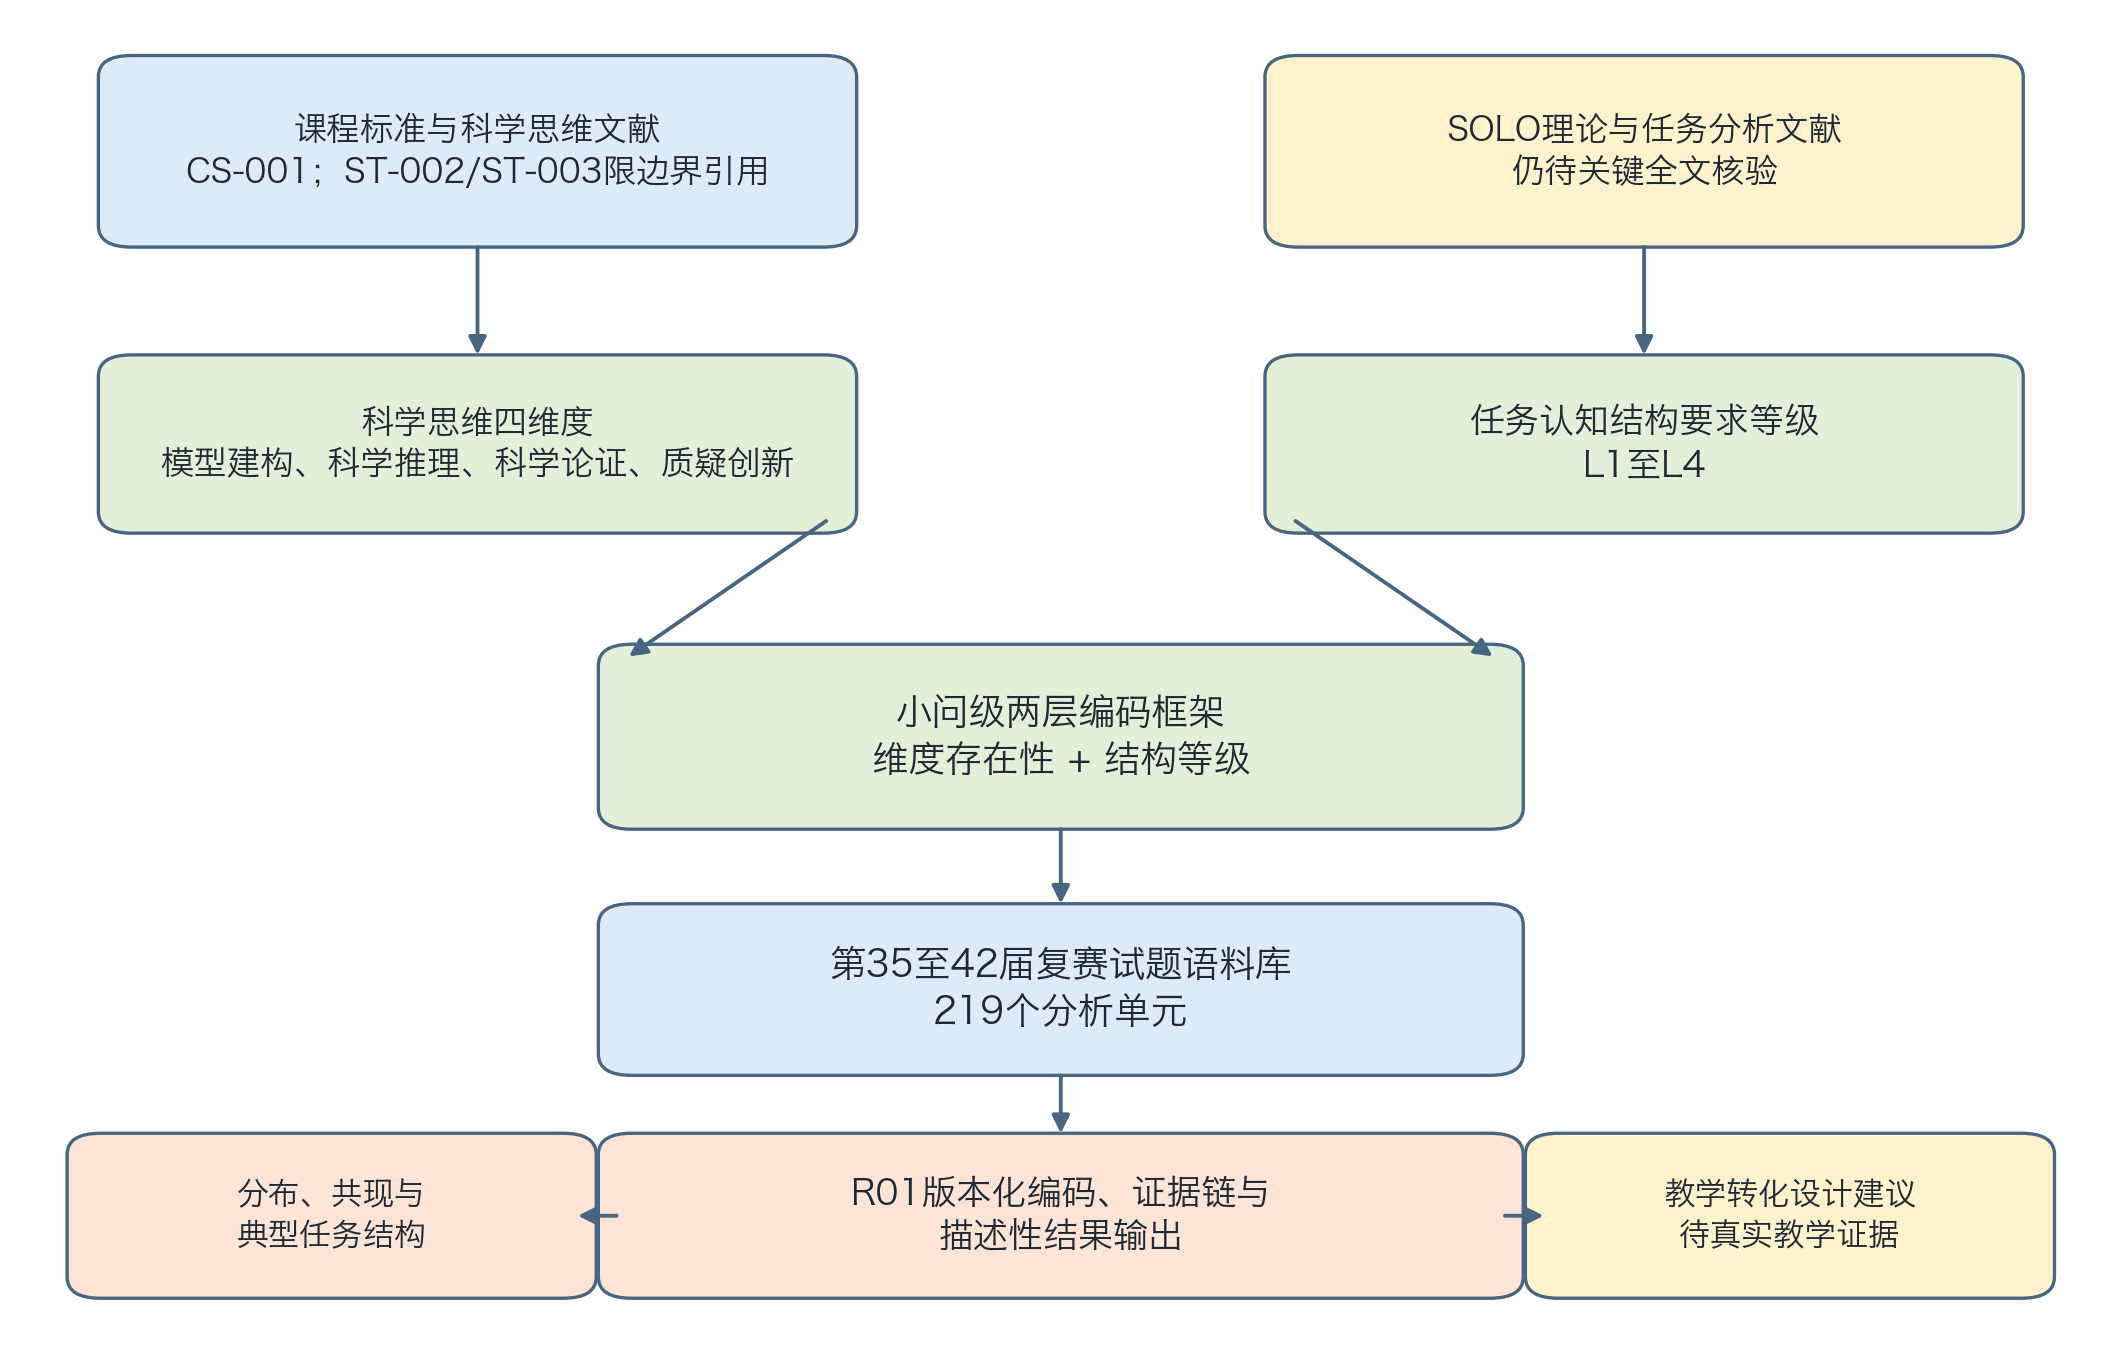
\includegraphics[keepaspectratio]{08_manuscript/figures/figure_2_1_r01_theoretical_framework_v1.png}}

图2-1 试题任务认知要求分析的理论框架。

从图2-1可以看到，理论概念并不直接导出教学结论，而是需要经过操作化、语料编码和案例解释三个环节。课程标准和相关理论提供维度选择的依据，编码手册将抽象概念转化为可判定的规则，描述统计呈现全样本中的任务结构分布，案例分析再把分布中的典型结构还原为具体题设与解答。教学设计建议位于这一链条的末端，其作用是把已经识别的任务结构转化为可实施的学习活动，而不是把统计比例直接转换为教学成效。

这一框架的关键不在于给每道题贴上一个笼统的``高''或``低''标签，而在于将任务中的不同工作分别呈现出来。以一道含有近似条件的力学题为例，学生可能需要先确定系统与研究对象，这是模型建构；再将受力、运动关系与边界条件连成推演链，这是科学推理；若题目要求说明近似何时失效，则还涉及科学论证；若进一步要求改变限制条件并比较新的处理方案，才可能出现质疑创新。四类活动在实际求解中彼此衔接，但它们并不应因最终都写在同一份解答中而被混为一个难度分数。

两层编码还使同一知识内容能够被作出更细的区分。例如，光学题既可以要求在已给几何关系下直接推导，也可以要求比较不同光路、说明近轴近似的适用范围；电磁学题既可以要求调用场与力的关系，也可以要求在不同参数条件下重新选择模型。前者和后者使用的知识点可能相近，却对条件组织、关系整合和结论说明提出不同要求。只有将维度出现与结构等级分开记录，才可能在保持物理内容完整的同时说明这种差异。

从教学设计的角度看，框架提供的不是现成的学生评价等级，而是一种拆解任务的工具。教师可以据此决定一题的评讲重点是补充模型假设、梳理推理链、要求理由说明，还是安排改变条件后的再判断；学生的实际作品则需要另有材料和规则评价。把任务要求与学生表现区分开来，既避免将文本分析误作学习诊断，也使后续课堂研究拥有明确的观察起点。

\section{本章小结}\label{ux672cux7ae0ux5c0fux7ed3-1}

\subsection{本章总结}\label{ux672cux7ae0ux603bux7ed3-1}

本章从科学思维四维度、SOLO启发的任务认知结构要求、两层编码逻辑和案例解释路径四个方面建立分析框架。该框架将研究对象限定为试题任务要求，而不以题目文本替代学生真实能力；将维度存在性与结构等级分开记录，而不以综合总分覆盖不同性质的任务；将总体统计与具体物理案例相互连接，使后续教学设计能够回到可见的题设条件和解答关系。\textsuperscript{[1, 2, 3, 6]}

\chapter{研究设计与编码框架}\label{ux7814ux7a76ux8bbeux8ba1ux4e0eux7f16ux7801ux6846ux67b6}

\section{总体研究设计}\label{ux603bux4f53ux7814ux7a76ux8bbeux8ba1}

\subsection{研究思路与分析对象}\label{ux7814ux7a76ux601dux8defux4e0eux5206ux6790ux5bf9ux8c61}

本研究以第35至42届全国中学生物理竞赛复赛试题为分析对象，采用内容分析的方法，考察复赛试题在模型建构、科学推理、科学论证和质疑创新四个维度上呈现的任务认知要求。研究对象是试题及参考解答对解题者提出的认知活动要求，而非学生实际表现出的科学思维水平。科学推理和科学思维测评研究表明，学生能力判断需要专门测评任务、学生作答数据和模型检验；自由作答研究也以学生书面作答中的可见证据为编码对象。\textsuperscript{[2, 3, 18]}
因此，本文中的等级判断均表述为``试题认知结构要求''或``任务结构复杂性''。

研究已建立第35至42届试题语料库、编码手册、双人编码记录、分歧裁决记录和逐条题干---解答证据。本文将分析结果界定为可追溯的描述性结果，不将其等同于学生能力测量或教学效果证据。

为使研究设计与证据范围相对应，表3-1将本研究的材料层、编码层、分析层和教学转化层分开呈现。各层之间并不是从题目文本直接推到学生能力或教学效果的线性关系，而是通过明确的输入、输出和限制逐层衔接。

{\def\LTcaptype{none} % do not increment counter
\begin{longtable}[]{@{}
  >{\raggedright\arraybackslash}p{(\linewidth - 8\tabcolsep) * \real{0.2000}}
  >{\raggedright\arraybackslash}p{(\linewidth - 8\tabcolsep) * \real{0.2000}}
  >{\raggedright\arraybackslash}p{(\linewidth - 8\tabcolsep) * \real{0.2000}}
  >{\raggedright\arraybackslash}p{(\linewidth - 8\tabcolsep) * \real{0.2000}}
  >{\raggedright\arraybackslash}p{(\linewidth - 8\tabcolsep) * \real{0.2000}}@{}}
\toprule\noalign{}
\begin{minipage}[b]{\linewidth}\raggedright
层面
\end{minipage} & \begin{minipage}[b]{\linewidth}\raggedright
研究材料
\end{minipage} & \begin{minipage}[b]{\linewidth}\raggedright
分析产出
\end{minipage} & \begin{minipage}[b]{\linewidth}\raggedright
本文用途
\end{minipage} & \begin{minipage}[b]{\linewidth}\raggedright
不作的推断
\end{minipage} \\
\midrule\noalign{}
\endhead
\bottomrule\noalign{}
\endlastfoot
语料层 & 第35至42届复赛题面、参考解答与小问级元数据 &
219个分析单元及其定位入口 & 界定试题材料与分析范围 &
学生样本、学生成绩或命题长期趋势 \\
编码层 & 四维度规则、L1至L4规则、题干---解答证据 & 876条编码与判定依据 &
描述任务要求的出现、等级与组合 & 学生真实思维、框架外部效度 \\
分析层 & 编码表与统计程序 & 分布、等级、共现和分组表 &
当前语料的描述统计 & 显著性、因果、跨届普遍规律 \\
转化层 & 三个典型案例与教学设计 & 任务、支架和评价产出建议 &
教学设计建议 & 学生困难、教师共识或教学效果 \\
\end{longtable}
}

表3-1的分层也决定了论文的写作顺序：第四章只报告分析层结果，第五章只将结果转化为待实施的设计材料。任何未来学生、教师或课堂资料都必须形成独立的数据来源、伦理与分析链，不能以题目或参考解答编码替代。

\section{语料来源与分析单位}\label{ux8bedux6599ux6765ux6e90ux4e0eux5206ux6790ux5355ux4f4d}

\subsection{语料范围与小问级单位}\label{ux8bedux6599ux8303ux56f4ux4e0eux5c0fux95eeux7ea7ux5355ux4f4d}

本研究语料为项目归档的第35至42届复赛试题和参考答案PDF，并建立``复赛试题小问级索引表''，当前共包含219个分析单元。分析单位优先采用独立小问；若同一小问内部包含相对独立的任务，则进一步拆分为分析单元。每条记录均保留届次、年份、题号、小问号、试题页码、答案页码、知识模块、情境、表征、数学工具和答案结构等元数据。

相邻的物理教育内容分析研究也表明，分析单位应随研究问题与材料性质明确界定，并公开纳入、排除与样本边界；其以教材图件为单位的规则不能原样迁移到本研究的小问级竞赛任务。\textsuperscript{[19]}

相邻的中国物理考试题内容分析会将同一大题中可相对独立、且要求不同认知操作的任务分别登记，并把题目中的图、表或示意图是否构成任务条件、是否要求生成表征写入纳入规则。因此，本研究拆分复赛大题时，以题干、题图和参考解答能够分别定位为前提；图件只作为支持任务要求的证据之一，不因其形式本身自动触发某一科学思维维度或等级。\textsuperscript{[20]}

相邻的物理试题研究还把数值、公式、文字、概念、图像与由文字触发的视觉化作为可并存的呈现特征登记。其中，图像是否出现与题干是否还要求解题者进行空间想象并非同一判断。因此，本研究只将题图、题表、公式和文字说明作为可定位的任务材料证据；任何单一呈现形式都不自动决定某一科学思维维度或任务结构等级。\textsuperscript{[21]}

相邻的物理题文本分类研究提示，除公布语料范围和分析单位外，还应说明判定依据、示例及分歧处理；题目所要求的认知过程还会受先备知识和相似题经验等分析前提影响。故本研究保留题干---参考解答定位、编码手册版本和分歧裁决记录，并只把它们用于描述试题任务要求，不据此推定参赛者实际采用的策略、能力或学习结果。\textsuperscript{[22, 23]}

另一项中国物理考试文本研究将内容主题与认知要求分开编码，公开样本范围、条目拆分规则、编码示例和二维汇总方式。这提示本研究应交代小问级分析单位、维度判据与汇总过程；但其SEC模型、认知水平定义、高考样本、一致性系数和命题建议均不迁移到本研究的竞赛语料。\textsuperscript{[24]}

语料整理过程中，对OCR文本、公式与特殊符号、题图裁边与图注以及第35届分值边界进行了人工校对。校对结果与题干、参考解答和图件材料相互对应，为后续编码提供了清晰的文本基础。

第35届评分标准副本记录了26个小问的分值分布。由于其他届次缺少可比的逐小问分值资料，本文不以分值作为全样本的主分析权重，也不据此进行跨届比较或趋势推断。

\subsection{小问拆分与元数据记录}\label{ux5c0fux95eeux62c6ux5206ux4e0eux5143ux6570ux636eux8bb0ux5f55}

小问级分析的关键不在于将题目机械切碎，而在于保持任务边界与物理意义的一致。对于题干中已经标明的（1）、（2）等子问，通常以子问作为分析单位；若某一子问包含前后相对独立的任务，且后半部分需要重新组织对象、条件或目标量，则将其拆分为相互可定位的分析单元。反之，若若干计算步骤只是围绕同一待求量连续展开，则仍视为一个分析单元。拆分后每个单元均保留与原题号、小问号和页码的对应关系，以保证统计结果能够回到原始题面。

元数据记录服务于后续检索和描述，而不直接作为任务结构等级的替代指标。知识模块用于说明题目涉及的主要物理内容；情境字段记录装置、过程或问题背景；表征字段记录文字、图像、表格、符号等材料形式；数学工具字段记录方程、函数、微积分、几何或其他工具性要素；答案结构字段概括参考解答的主要组织方式。上述字段可以帮助比较不同材料条件下的编码分布，也可以支持案例抽取，但不应据此直接断言某一知识模块或表征形式必然导致更高或更低的科学思维要求。

为降低拆分和元数据记录带来的任意性，研究记录同时保存题面页、答案页、题图或表格定位以及相应的文字说明。这样，当某一统计数字或案例解释需要复查时，可以先定位到分析单元，再回到题干、参考解答和图件材料，而不是只依据汇总表进行二次解释。小问级索引由此构成语料层与编码层之间的连接点。

\section{编码手册开发}\label{ux7f16ux7801ux624bux518cux5f00ux53d1}

\subsection{编码维度与判定规则}\label{ux7f16ux7801ux7ef4ux5ea6ux4e0eux5224ux5b9aux89c4ux5219}

编码框架以科学思维四维度为主体，并引入SOLO理论作为``任务认知结构要求''等级划分的启发来源。编码手册规定每个维度分别判断``是否出现''和``出现时的等级''，避免把计算复杂度、背景陌生度或参考解答篇幅直接等同于高阶思维要求。

四个维度的操作性边界如下。模型建构关注研究对象、系统边界、变量、理想化假设和模型形成；科学推理关注由条件到结论的物理关系链；科学论证关注比较、检验、边界分析和假设辩护；质疑创新仅在题目明确要求处理假设、替代模型、模型失效、开放方案或证据约束的新方案时触发。等级从L1至L4表示任务结构复杂性递增，但不表示学生真实学习结果等级。

编码手册配套保存双人编码的876条记录、142条分歧讨论记录和4条更正记录，并据此报告一致性结果和分歧处理过程。一致性统计用于说明编码判断的一致程度，不作为框架外部效度的唯一依据。

编码时先判断某维度是否出现，再对``出现''的记录判定L1至L4；若未出现，则等级固定为``未出现''。每条记录均要求保留题干触发语、题面定位、解答关键步骤、答案定位和相邻等级排除说明。这样的记录结构使``存在性判断''\,``等级判断''和``证据定位''能够分别审阅，避免用一个笼统的难度标签覆盖不同性质的判断。

\section{专家审查}\label{ux4e13ux5bb6ux5ba1ux67e5}

\subsection{框架审阅与修订}\label{ux6846ux67b6ux5ba1ux9605ux4e0eux4feeux8ba2}

本研究已完成编码框架的专家审阅与研究者复核，并据此形成编码手册和编码表。专家审阅聚焦四个维度的操作性定义、等级边界和样本编码的适切性；相关审阅材料和修订记录保存在研究档案中。为保证表述边界，专家审阅用于支持框架的内容适切性，不替代对学生能力、教学效果或因果关系的实证检验。

\section{试编码与评分者一致性}\label{ux8bd5ux7f16ux7801ux4e0eux8bc4ux5206ux8005ux4e00ux81f4ux6027}

\subsection{一致性分析}\label{ux4e00ux81f4ux6027ux5206ux6790}

在正式编码前，研究者以219个分析单元形成876条预编码记录，用于发现规则边界和证据表述中的问题。预编码记录不直接用于第四章统计。

两名编码者分别对876条维度记录进行判断，研究据此计算维度存在性一致率、Cohen's
kappa、等级一致率和二次加权kappa。对142条分歧逐条讨论后形成基础编码表，并在复核中修订4条记录。一致性统计用于说明编码判断的相符程度；内容分析方法文献支持按变量报告一致性、说明指标选择并保留分歧处理记录的原则。\textsuperscript{[6]}

对于两名评分者的分类记录，原始一致率呈现直接观察到的同判比例，kappa类指标则尝试校正机会一致；两者均须结合比较数、类别分布和评分者独立性假定解释。Cohen关于名义分类一致性的原始讨论把独立单元、互斥且穷尽的类别及独立评分者列为适用前提；Landis与Koch给出的解释性区间也明确只是便于讨论的任意基准。故本项目同时保留原始一致与kappa类统计，且不把任何历史区间设为通过线；评分过程只能按自声明登记的限制仍写入方法边界。这些统计不构成框架效度或评分过程独立性的证明。\textsuperscript{[25, 26, 27]}

表3-2列出双人编码的一致性结果。存在性统计的比较数为全部876对维度记录；等级统计只在双方均判断该维度出现时计算。因此，两个部分的分母不同，不应将等级kappa与存在性kappa直接作高低排序。

{\def\LTcaptype{none} % do not increment counter
\begin{longtable}[]{@{}
  >{\raggedright\arraybackslash}p{(\linewidth - 12\tabcolsep) * \real{0.1111}}
  >{\raggedleft\arraybackslash}p{(\linewidth - 12\tabcolsep) * \real{0.1481}}
  >{\raggedleft\arraybackslash}p{(\linewidth - 12\tabcolsep) * \real{0.1481}}
  >{\raggedleft\arraybackslash}p{(\linewidth - 12\tabcolsep) * \real{0.1481}}
  >{\raggedleft\arraybackslash}p{(\linewidth - 12\tabcolsep) * \real{0.1481}}
  >{\raggedleft\arraybackslash}p{(\linewidth - 12\tabcolsep) * \real{0.1481}}
  >{\raggedleft\arraybackslash}p{(\linewidth - 12\tabcolsep) * \real{0.1481}}@{}}
\toprule\noalign{}
\begin{minipage}[b]{\linewidth}\raggedright
范围
\end{minipage} & \begin{minipage}[b]{\linewidth}\raggedleft
存在性比较数
\end{minipage} & \begin{minipage}[b]{\linewidth}\raggedleft
存在性一致率
\end{minipage} & \begin{minipage}[b]{\linewidth}\raggedleft
Cohen's kappa
\end{minipage} & \begin{minipage}[b]{\linewidth}\raggedleft
等级比较数
\end{minipage} & \begin{minipage}[b]{\linewidth}\raggedleft
等级一致率
\end{minipage} & \begin{minipage}[b]{\linewidth}\raggedleft
二次加权kappa
\end{minipage} \\
\midrule\noalign{}
\endhead
\bottomrule\noalign{}
\endlastfoot
全部 & 876 & 96.12\% & 0.9053 & 607 & 82.21\% & 0.8638 \\
模型建构 & 219 & 98.63\% & 0.8893 & 203 & 82.76\% & 0.8989 \\
科学推理 & 219 & 100.00\% & 1.0000 & 219 & 81.74\% & 0.7674 \\
科学论证 & 219 & 95.43\% & 0.9084 & 98 & 82.65\% & 0.4494 \\
质疑创新 & 219 & 90.41\% & 0.8059 & 87 & 81.61\% & 0.8905 \\
\end{longtable}
}

表3-2不以任何外部阈值将结果简单判为``优秀''或``合格''。尤其科学论证的等级比较仅有98对，其等级加权kappa应结合样本量、分歧类型和具体题目材料理解。研究保留分歧讨论记录，而不以一个总体指标替代边界案例的复核。

\subsection{一致性结果的解释}\label{ux4e00ux81f4ux6027ux7ed3ux679cux7684ux89e3ux91ca}

原始一致率与kappa类指标回答的并不是同一个问题。原始一致率呈现两名编码者在全部比较记录中作出相同判断的比例，直观反映编码记录的相符程度；Cohen's
kappa则在名义分类条件下对机会一致进行校正；二次加权kappa用于等级有序、且相邻等级差异小于跨级差异的情形。三类指标共同使用，可以避免只凭某一个数字判断编码质量。\textsuperscript{[25, 26, 27]}

表3-2显示，四个维度的存在性一致率整体高于等级一致率。这一差异符合两层编码的逻辑：判断某一维度是否出现，通常依据较明确的题干要求和解答结构；在已经判定维度出现后，再区分L1至L4，需要对条件数量、关系组织、边界分析和迁移要求作更细的解释，因此更容易产生等级边界分歧。等级分歧并不必然意味着编码框架无效，而是提示需要回到具体证据，检查判定规则是否清楚、相邻等级是否可区分。

不同维度的一致性也应结合其任务特点理解。科学推理在全体分析单元中均被判为出现，存在性判断的类别分布较为集中，等级判断则仍涉及从直接关系调用到多条件整合的区分。科学论证的等级比较数相对较少，相关系数更容易受到样本量和类别分布影响，因此不能只据一个系数对该维度作强结论。质疑创新的出现数较少，判定重点又涉及``题目是否明确要求假设处理、替代方案或模型修正''，需要通过题干和解答的具体证据避免把新颖背景或复杂计算误判为创新要求。

分歧裁决的作用在于把统计层面的不一致重新带回题目材料。对于每一条分歧，裁决需要核对题干的触发语、参考解答的关键步骤、相邻等级排除理由以及编码手册中的边界规定。经裁决后的编码表用于第四章的统计与案例分析，而原始编码记录和分歧记录仍保留为理解规则修订过程的材料。这样的处理使一致性检验不止产生一个汇总指标，也促成编码框架在具体边界问题上的完善。

\section{正式编码与数据处理}\label{ux6b63ux5f0fux7f16ux7801ux4e0eux6570ux636eux5904ux7406}

\subsection{编码流程与统计处理}\label{ux7f16ux7801ux6d41ux7a0bux4e0eux7edfux8ba1ux5904ux7406}

编码流程包括独立判断、字段检查、一致性计算、分歧讨论、复核修订和统计输出六个步骤。对于引文不足、题干与解答对应不清或边界较为复杂的记录，研究回到原题和参考解答补充依据后再作判断。最终形成876条编码记录，并据此生成总体分布、等级分布、共现关系和分组表。\textsuperscript{[6]}

除届次和知识模块外，项目还保留题面表征、数学工具和答案结构等小问级元数据。由于这些字段的原始表述多按具体题材登记，不能把60种具体描述强行归成未经审查的少数主题。为保持口径透明，本文仅将``表征''和``数学工具''字段以全角分号分隔的非空要素数作机械计数，生成``表征要素分层描述表''和``数学工具要素分层描述表''。该计数只描述索引记录的结构，不测量题目难度、数学复杂度、认知负荷或学生能力；第四章仅在样本数不少于30的分层中作定位性呈现，完整小样本层仍保留于数据表输出。

当前结果使用的版本并不是最早生成的基线表。复核后共采纳4条更正：其中1条将模型建构由L3调整为L1，3条将原先判为质疑创新的记录调整为未出现。因此，当前唯一分析输入为``当前更正编码表''；更正前的基线编码表和历史描述输出只保留作版本复现，不得用于第四章、摘要或结论。更正后质疑创新出现数为84，模型建构L3为72，质疑创新L4为8，所有描述表均以该更正版本重建。

数据处理的最小复跑路径是：先校验当前编码表和证据链的876个唯一键及逐键值一致性，再核验描述统计输出的输入哈希，最后将正文表格、图件和案例与当前输出对齐。元数据要素数分层还同时记录``复赛试题小问级索引表''与当前编码表的SHA-256，以防语料元数据和编码表在不同版本间错配。该路径的用途是防止历史基线表、局部更正和正文数字发生版本错配；它不替代对原始人工过程或理论框架的外部审查。

\subsection{描述统计与结果解释}\label{ux63cfux8ff0ux7edfux8ba1ux4e0eux7ed3ux679cux89e3ux91ca}

本研究以小问等权作为全样本的基本统计口径。对于每个维度，首先统计被判定为``出现''的分析单元数及其占219个分析单元的比例；对于等级分布，则以该维度已经出现的单元数为分母，分别呈现L1至L4的构成。由于同一小问可以同时包含多个科学思维维度，四个维度的出现数不相互排斥，也不相加构成所谓``总思维分''。

维度共现分析用于描述同一分析单元内两类任务要求的同时出现情况。本文报告交集、并集和Jaccard系数，以展示不同维度在当前语料中的组合关系。Jaccard系数反映集合重叠程度，不能替代相关系数、效应量或因果指标。届次、知识模块、表征要素和数学工具要素的分层统计同样用于呈现材料结构与编码分布，重点是为进一步的案例阅读和教学设计提供检索入口，而不是检验跨届趋势或组间显著性差异。

结果解释遵循``统计表---题干与解答---案例材料''的顺序。统计表回答总体上出现了什么，题干与参考解答说明某一判定在何种任务结构中产生，案例分析则将这些结构转换为可讨论的教学任务。通过这一顺序，描述性统计既保持全样本视野，也避免将抽象比例脱离具体物理情境进行解释。

这一统计口径特别重视分母的可解释性。维度出现比例以219个分析单元为共同分母，回答的是某类任务要求在全部小问中出现的范围；等级构成则以相应维度已经出现的单元为分母，回答的是该类任务内部的结构分布。二者不能混用。例如，科学论证的等级构成只应在已经出现科学论证要求的小问中理解，不能把其L1、L2、L3直接除以全样本后与其他维度作``高低''比较。将分母写清楚，是避免统计表被误读为学生能力比例或总难度分布的基本条件。

共现分析也遵循同样的克制原则。若模型建构与科学推理在同一单元中共同出现，所能说明的是该单元的完成同时需要组织模型与推演关系；它不能证明两个维度在心理机制上必然相关，更不能说明学生掌握其中一个维度后必然掌握另一个维度。Jaccard系数用于展示两个集合的重叠程度，其解释仍须回到具体题目中条件、模型和推导的组织方式。因而，本研究把共现表视为案例检索工具，而不是对变量关系进行因果解释的证据。

对于届次和元数据分层，本文采用``先报告结构、后核对材料''的阅读原则。某个分层中的比例若值得讨论，首先应检查该层的样本量、包含的题目和小问拆分方式；其次应回到题干和解答确认是否存在相似的任务机制；最后才判断其能否形成教学选题线索。这样既可以利用分层表发现条件链、状态分类或近似处理较集中的题目，又能避免由少量小问或表面材料特征推出过强结论。

第四章报告基于试题文本的描述性结果，不报告显著性检验、因果推断、学生能力、教学效果或长期趋势；第五章据此提出教学设计建议，不将编码结果直接解释为课堂成效。

\section{教师/课堂研究设计}\label{ux6559ux5e08ux8bfeux5802ux7814ux7a76ux8bbeux8ba1}

\subsection{教学转化设计}\label{ux6559ux5b66ux8f6cux5316ux8bbeux8ba1}

教学转化部分采用``结果---问题---策略---任务---评价''的链条，将试题分析结果转化为竞赛教学中的任务设计、支架设计和评价量规。科学论证教学研究和国际科学实践框架为任务、支架和评价对象提供设计参照。\textsuperscript{[4, 5]}
本文提出教学转化设计框架，不将其表述为已经验证的教学效果。

若后续采用稳健型路线，可优先补充教师访谈、教学案例评审或小范围教师咨询；若采用进阶型路线，则需要至少两轮真实课堂设计、实施、反思和修订，并保存学生作品、课堂观察和实施偏离记录。

\section{伦理与质量控制}\label{ux4f26ux7406ux4e0eux8d28ux91cfux63a7ux5236}

\subsection{研究质量控制}\label{ux7814ux7a76ux8d28ux91cfux63a7ux5236}

本研究当前阶段主要使用公开或用户提供的竞赛试题材料，不涉及学生个人数据。若后续进入教师访谈、问卷或课堂研究，应补充知情说明、匿名化规则、数据保存方式和伦理风险说明。所有教师、学生、课堂、问卷和访谈数据均不得由研究者或工具生成替代。

质量控制包括四个层面。第一，语料层面保留原始PDF、题干文本、题图资产和校对记录；第二，框架层面保留编码手册、判定规则和预编码记录；第三，编码层面保留双人编码记录、分歧讨论和修订结果，并说明一致性样本、指标、训练和分歧处理；\textsuperscript{[6]}
第四，分析层面以统计程序生成结果表，避免手工计算导致不可复核。

\subsection{语料与文本质量控制}\label{ux8bedux6599ux4e0eux6587ux672cux8d28ux91cfux63a7ux5236}

语料质量控制首先关注材料边界是否清楚。每份试题和参考答案均以届次、题号、页码和文件校验信息登记，题干与解答文本分别保留，以避免将题目要求与参考答案步骤混为同一材料。对于公式、特殊符号、图件裁边或答案页边界等容易影响理解的内容，研究记录保留相应的校对入口和定位信息。这样做的目的不是把文本处理过程写成研究发现，而是保证后续编码能够回到足以判断任务要求的材料。

第二，文本质量控制关注分析单位与原始材料之间的对应。每个分析单元都保留其所属大题、小问、题面页和答案页，使小问拆分不会脱离原题语境。若一个统计结果或案例解释涉及图像、公式或条件限制，读者可以沿索引回查相应材料。对内容分析而言，这种可回查性比单纯扩大样本数量更重要，因为它使研究者能够发现并修正拆分、转写或定位中的问题。

\subsection{编码与分析质量控制}\label{ux7f16ux7801ux4e0eux5206ux6790ux8d28ux91cfux63a7ux5236}

编码质量控制强调规则、证据和版本之间的一致。编码手册明确维度定义、等级含义、排除规则和边界情形；每条编码记录同时保存题干触发语和解答关键步骤；出现分歧时，先回到材料和规则，而不是只根据统计结果调整判断。这样的流程使``为什么这样编码''能够得到具体回答，也使后续修订能够定位受影响的单元与维度。

分析质量控制则避免正文数字与输入数据脱节。总体分布、等级分布、维度共现和分层表均由当前编码表重新计算，图件、表格和案例选择与同一版本的结果保持对应。当编码值发生更正时，需要同步检查描述统计、图件和正文解释是否仍然一致。可复现并不意味着研究结论永远不变，而是意味着结论变化时能够清楚说明变化来自哪一条规则、哪一份材料或哪一项编码修订。

在论文写作中，质量控制还表现为主张强度与证据类型相匹配。题干和参考解答可以支持对任务要求的描述，编码和统计可以支持对当前语料分布的概括，教学设计材料可以支持对任务、支架和评价方式的建议；这些材料不能替代学生作答、教师访谈或课堂实施数据。将不同证据类型分层处理，有助于保持论文结论的准确性，也为后续研究提供明确的扩展方向。

\section{本章小结}\label{ux672cux7ae0ux5c0fux7ed3-2}

\subsection{本章总结}\label{ux672cux7ae0ux603bux7ed3-2}

本章说明了研究设计、语料来源、分析单位、编码框架、编码流程和质量控制方案。基于小问级语料、双人编码、分歧讨论和题干---解答证据，下一章将报告复赛试题科学思维要求的描述性结果。

本文不将试题编码结果推断为学生能力、教学效果、因果关系、显著性差异或长期命题趋势。若编码规则或具体判断发生修订，应同步检查统计输出、表格、图件和正文解释。

\chapter{试题科学思维要求的分析结果}\label{ux8bd5ux9898ux79d1ux5b66ux601dux7ef4ux8981ux6c42ux7684ux5206ux6790ux7ed3ux679c}

本章以219个分析单元的876条维度编码记录为基础，报告复赛试题在模型建构、科学推理、科学论证和质疑创新四个维度上的任务要求分布。编码记录均保留题干与参考解答的定位依据。结果反映试题任务结构，不代表学生实际能力或教学效果。

\section{样本、编码与结果边界}\label{ux6837ux672cux7f16ux7801ux4e0eux7ed3ux679cux8fb9ux754c}

\subsection{样本与编码概况}\label{ux6837ux672cux4e0eux7f16ux7801ux6982ux51b5}

本研究以第35至42届复赛试题中的独立小问为分析单位，共219个分析单元。围绕模型建构、科学推理、科学论证和质疑创新四个维度，共形成876条编码记录。两名编码者在维度存在性判断上的一致率为96.12\%，Cohen's
kappa为0.9053；在双方均判断维度出现的607对记录中，等级一致率为82.21\%，二次加权kappa为0.8638。对142条分歧进行讨论和裁决后，形成用于统计分析的最终编码表。

编码过程中，对存在分歧、引文不足或边界较为复杂的记录进行了重点复核，并依据题干、参考解答和编码规则完成修订。最终编码表中的每一条记录均可回到相应的题面和解答材料。本文据此开展描述性统计，重点呈现各维度的出现情况、等级构成、组合关系和案例机制。

下述全样本结果限定于本语料和本编码手册，并以小问等权为主分析口径。全样本主分析不进行分值加权。仅第35届留有逐小问分值资料副本，且其发布/授权链未由项目独立核验，故不将其纳入主分析，也不开展分值加权、跨届比较、趋势、学生成绩或能力推断；本章同样不进行显著性检验、因果推断或长期趋势判断。

\section{四维度出现情况}\label{ux56dbux7ef4ux5ea6ux51faux73b0ux60c5ux51b5}

\subsection{维度出现比例}\label{ux7ef4ux5ea6ux51faux73b0ux6bd4ux4f8b}

表4-1呈现四个维度在219个分析单元中的出现情况。

{\def\LTcaptype{none} % do not increment counter
\begin{longtable}[]{@{}lrrr@{}}
\toprule\noalign{}
维度 & 出现单元数 & 总单元数 & 出现比例 \\
\midrule\noalign{}
\endhead
\bottomrule\noalign{}
\endlastfoot
模型建构 & 203 & 219 & 92.69\% \\
科学推理 & 219 & 219 & 100.00\% \\
科学论证 & 106 & 219 & 48.40\% \\
质疑创新 & 84 & 219 & 38.36\% \\
\end{longtable}
}

在本语料和本编码口径下，科学推理被判为出现于全部219个分析单元，模型建构出现于203个单元；科学论证与质疑创新分别出现于106个和84个单元。这些比例用于描述试题及其参考解答要求何种认知活动，不能被解释为学生在四个维度上的真实优势、短板或学习结果。

科学推理在全部分析单元中出现，说明复赛小问普遍要求解题者在题设条件、物理规律和目标量之间建立明确关系。模型建构出现于203个单元，显示多数小问还要求对研究对象、变量、条件或近似作出组织；其余16个单元则主要沿用题目已经给定的模型推进推理。科学论证和质疑创新的出现比例相对较低，表明这两类要求更集中于需要比较、检验、讨论或方案调整的特定任务，而不是每一道计算题的必经环节。

这种分布为理解复赛题的任务结构提供了一个切入点：复赛试题并非简单地由高难度计算构成，而是以科学推理为基本骨架，在不同小问中叠加模型建构、论证或创新要求。后续案例分析将进一步说明，这些维度在具体题设中如何通过条件设置、状态分类和近似假设表现出来。

从记录数看，科学推理与模型建构之间相差16个分析单元，说明多数小问同时包含模型识别或组织与关系推演，但这一差额仍保留了``由既定模型直接推进关系''的单元。科学论证与质疑创新的出现数分别比科学推理少113个和135个单元。这里的``少''仅是当前手册下的任务要求出现次数差异，不表示某类能力更重要、某类试题更难，亦不能替代对题干措辞、参考解答结构和具体物理内容的逐题阅读。

四维度的分母相同，因此表4-1可作同一语料内的出现频数比较；但它不能把不同维度相加为``总思维分''，也不能将同一小问中的多个维度视为相互排斥。后续的等级和共现结果正是分别处理这两个问题：前者只在维度已经出现时判断任务结构，后者则保留同一小问可以同时提出多类要求的事实。

\noindent\pandocbounded{\includegraphics[keepaspectratio]{/Users/dongxingxi/physics_competition_thesis_excellent_v2/08_manuscript/figures/figure_4_1_dimension_presence_r01_v1.png}}

图4-1
四维度在219个分析单元中的出现比例。图件由当前更正编码表及其已核验描述统计直接生成。

\subsection{四维度的任务功能}\label{ux56dbux7ef4ux5ea6ux7684ux4efbux52a1ux529fux80fd}

四维度在全样本中的出现范围不同，反映的并不是哪一种能力``更重要''，而是复赛小问在完成方式上的功能分工。科学推理出现于全部分析单元，说明每个小问都需要把条件、规律与目标量连接起来；模型建构出现于203个单元，说明大多数小问还要求解题者明确系统、变量、状态或近似条件。对于其余16个单元，任务的主要结构更接近在题目已经给定的模型中推进关系，而不是重新选择或组织模型。

科学论证和质疑创新的功能与前两者不同。科学论证出现于106个单元，通常使任务从``得到结论''继续走向``说明结论为何成立、比较对象是否一致或适用条件为何成立''；质疑创新出现于84个单元，通常要求解题者面对条件改变、替代方案或模型边界。二者出现频数低于科学推理，并不意味着其在完整物理分析中只是可有可无的附加环节，而是说明它们更多集中在具有比较、检验、修正或设计要求的小问中。

从题目组织的角度看，四维度共同构成一种可递进展开的任务结构。题面先通过对象、条件和限制确定可讨论的物理系统，随后由规律关系将已知量推向目标量；当题目要求解释比较结果或检查近似时，任务进入论证；当原有条件被改变或需要提出可行路径时，任务才可能进入质疑创新。实际小问并不一定按这一顺序书写，四个维度也不构成固定的阶段序列，但这一功能区分有助于解释为什么同样是``计算题''，有的重点在条件组织，有的重点在结论说明，还有的重点在改变假设后的重建。

\section{等级分布}\label{ux7b49ux7ea7ux5206ux5e03}

\subsection{各维度等级构成}\label{ux5404ux7ef4ux5ea6ux7b49ux7ea7ux6784ux6210}

表4-2的分母为每一维度被判定为``出现''的分析单元数，而不是219个全部分析单元。

{\def\LTcaptype{none} % do not increment counter
\begin{longtable}[]{@{}
  >{\raggedright\arraybackslash}p{(\linewidth - 10\tabcolsep) * \real{0.1304}}
  >{\raggedleft\arraybackslash}p{(\linewidth - 10\tabcolsep) * \real{0.1739}}
  >{\raggedleft\arraybackslash}p{(\linewidth - 10\tabcolsep) * \real{0.1739}}
  >{\raggedleft\arraybackslash}p{(\linewidth - 10\tabcolsep) * \real{0.1739}}
  >{\raggedleft\arraybackslash}p{(\linewidth - 10\tabcolsep) * \real{0.1739}}
  >{\raggedleft\arraybackslash}p{(\linewidth - 10\tabcolsep) * \real{0.1739}}@{}}
\toprule\noalign{}
\begin{minipage}[b]{\linewidth}\raggedright
维度
\end{minipage} & \begin{minipage}[b]{\linewidth}\raggedleft
出现数
\end{minipage} & \begin{minipage}[b]{\linewidth}\raggedleft
L1
\end{minipage} & \begin{minipage}[b]{\linewidth}\raggedleft
L2
\end{minipage} & \begin{minipage}[b]{\linewidth}\raggedleft
L3
\end{minipage} & \begin{minipage}[b]{\linewidth}\raggedleft
L4
\end{minipage} \\
\midrule\noalign{}
\endhead
\bottomrule\noalign{}
\endlastfoot
模型建构 & 203 & 109 (53.69\%) & 22 (10.84\%) & 72 (35.47\%) & 0
(0.00\%) \\
科学推理 & 219 & 121 (55.25\%) & 81 (36.99\%) & 17 (7.76\%) & 0
(0.00\%) \\
科学论证 & 106 & 79 (74.53\%) & 16 (15.09\%) & 11 (10.38\%) & 0
(0.00\%) \\
质疑创新 & 84 & 20 (23.81\%) & 51 (60.71\%) & 5 (5.95\%) & 8 (9.52\%) \\
\end{longtable}
}

在各维度被判为出现的单元中，模型建构、科学推理和科学论证的L1占比均最高；质疑创新以L2占比最高。这里的L1至L4仅表示SOLO启发的任务认知结构要求，不能等同于题目难度、学生作答质量或学生实际学习结果。

模型建构的L1和L3分别为109个和72个单元，L2为22个单元，未出现L4；这表明当前规则下，模型建构既包括直接调用标准模型的任务，也包括需要整合过程、边界或假设的任务。科学推理的L1、L2和L3分别为121、81和17个单元，等级记录主要集中在前两级。科学论证在106个出现单元中有79个L1、16个L2和11个L3；质疑创新在84个出现单元中则以51个L2最多，另有20个L1、5个L3和8个L4。上述构成只是在``该维度已出现''条件下的内部结构描述，不能据此跨维度比较所谓``高阶程度''，因为各维度的纳入条件和出现基数不同。

尤其需要避免把L4记录数为零或较少直接解释为试题``缺少高阶性''。L4是本项目为迁移、修正、一般化或开放构造等明确任务要求设置的保守判定，不是对题目总体质量的评分；不同维度是否允许L4、何种题设证据足以触发L4，仍受当前操作化规则和理论取舍限制。

从等级构成看，模型建构中L1与L3同时占有较大比例，反映复赛题中既有直接调用标准模型的任务，也有需要整合对象、条件、过程或边界的任务。科学推理以L1和L2为主，说明多数小问要求在明确规律和题设之间建立关系，部分小问则需要同时处理多个条件或关系；L3所占比例较小，主要对应需要把多个物理关系、数学工具和限制条件组织为连续推演链的任务。

科学论证的L1比例较高，表明该维度出现时常以局部的比较、检验或适用条件说明为主要形式。质疑创新则以L2比例最高，说明相关任务往往不只是提出一个新设想，而是要求在既定约束下并列处理多个假设、条件或方案。这里的等级构成不宜跨维度作简单排序：各维度的触发条件、可用等级和出现基数不同，L2在一个维度中的含义也不能直接等同于另一个维度中的L2。

等级分布的教学意义在于帮助教师识别任务中需要额外显性化的环节。若一个小问的科学推理表现为L3，教学中可要求学生展示条件、规律和中间关系的连接；若模型建构表现为L3，则可要求学生说明对象、假设和变量如何共同构成模型；若质疑创新进入较高等级，则可设计替代方案、修正假设或比较限制条件的追问。通过把等级还原为具体任务结构，等级统计才能成为选题与改题的参考。

\noindent\pandocbounded{\includegraphics[keepaspectratio]{/Users/dongxingxi/physics_competition_thesis_excellent_v2/08_manuscript/figures/figure_4_2_level_distribution_r01_v1.png}}

图4-2
四维度的等级构成。各横条以该维度被判为出现的单元数为分母，故不用于比较四个维度的绝对出现数量。

\subsection{模型建构与科学推理的等级组配}\label{ux6a21ux578bux5efaux6784ux4e0eux79d1ux5b66ux63a8ux7406ux7684ux7b49ux7ea7ux7ec4ux914d}

模型建构与科学推理共同出现于203个单元。为进一步观察两类任务要求如何在同一小问中配合，表4-3列出模型建构等级与科学推理等级的组配频数。该表的每一格都是同一分析单元中的两条维度记录，不是相关系数，也不表示两个等级能够相互替代。

{\def\LTcaptype{none} % do not increment counter
\begin{longtable}[]{@{}lrrrr@{}}
\toprule\noalign{}
模型建构等级 & 科学推理L1 & 科学推理L2 & 科学推理L3 & 合计 \\
\midrule\noalign{}
\endhead
\bottomrule\noalign{}
\endlastfoot
L1 & 56 & 44 & 9 & 109 \\
L2 & 11 & 11 & 0 & 22 \\
L3 & 39 & 26 & 7 & 72 \\
合计 & 106 & 81 & 16 & 203 \\
\end{longtable}
}

表4-3显示，模型建构L1与科学推理L1或L2的组配分别为56个和44个单元，构成较为常见的任务形态：模型或研究对象相对明确，但仍需要在一个或多个条件下建立关系。模型建构L3与科学推理L1、L2、L3的组配分别为39个、26个和7个单元，表明较高的模型组织要求并不必然伴随同等级的长推演链。有些小问的主要难点在于确定对象、状态、边界或近似，一旦模型确定，后续推理可以相对直接；另一些小问则需要同时组织模型和多重关系。

科学推理L3在表中的16个单元分布于模型建构L1和L3，分别为9个和7个单元，模型建构L2与科学推理L3的组配为0。这一结果只描述当前语料和编码规则下的记录分布，不应解释为某种普遍的阶段规律。它提示研究者和教师在阅读高关系整合要求的小问时，不能只看公式链是否较长，还要检查模型是否已在题面中明确给定；同样，面对模型建构L3的小问，也需要区分其后续推演是直接关系调用还是多条件整合。

等级组配的教学意义在于使支架更有针对性。对于``模型建构L3---科学推理L1''的任务，教师可重点要求学生说明系统边界、状态条件或近似假设，而不必用冗长的关系图替代必要推导；对于``模型建构L1---科学推理L3''的任务，则更适合要求学生画出条件---规律---中间量的关系链。只有将两类等级放在同一任务中阅读，等级统计才可能转化为具体的选题和评讲依据。

\noindent\pandocbounded{\includegraphics[keepaspectratio]{/Users/dongxingxi/physics_competition_thesis_excellent_v2/08_manuscript/figures/figure_4_3_model_reasoning_level_pair_r01_v1.png}}

图4-3
模型建构与科学推理的等级组配。图中每个数字代表同时具有相应两类等级要求的分析单元数，依据当前更正编码表生成。

\section{维度组合与共现}\label{ux7ef4ux5ea6ux7ec4ux5408ux4e0eux5171ux73b0}

\subsection{维度共现特征}\label{ux7ef4ux5ea6ux5171ux73b0ux7279ux5f81}

模型建构与科学推理共同出现203个分析单元；科学论证与质疑创新共同出现40次，两者并集为150个单元，Jaccard系数为0.2667。其余维度对的复算结果见``维度共现描述统计表''。

为便于在同一口径下观察各维度对的交集与并集，表4-4列出全部六组组合。模型建构与科学推理的共同出现数为203，等于模型建构的全部出现数；科学推理与科学论证、质疑创新的共同出现数分别为106和84，等于后两者的全部出现数。这些集合关系来自当前编码，不表示一个维度在理论上从属于另一个维度，而是提示在本语料的判定规则下，出现科学论证或质疑创新的单元同时也被判定包含科学推理。

{\def\LTcaptype{none} % do not increment counter
\begin{longtable}[]{@{}lrrr@{}}
\toprule\noalign{}
维度组合 & 同时出现数 & 至少出现一个的单元数 & Jaccard系数 \\
\midrule\noalign{}
\endhead
\bottomrule\noalign{}
\endlastfoot
模型建构---科学推理 & 203 & 219 & 0.9269 \\
模型建构---科学论证 & 106 & 203 & 0.5222 \\
模型建构---质疑创新 & 84 & 203 & 0.4138 \\
科学推理---科学论证 & 106 & 219 & 0.4840 \\
科学推理---质疑创新 & 84 & 219 & 0.3836 \\
科学论证---质疑创新 & 40 & 150 & 0.2667 \\
\end{longtable}
}

表4-4中的Jaccard系数只是集合重叠程度的描述指标，不是相关系数、效应量或因果指标。科学论证与质疑创新的交集为40个单元，既说明两类要求可共同出现，也保留了各自单独出现的情况：科学论证出现而质疑创新未出现的单元为66个，质疑创新出现而科学论证未出现的单元为44个。

共现表示同一任务同时被编码为包含两个维度的要求，不表示学生在这些维度上的同步发展，也不证明两个维度具有因果关系。

模型建构与科学推理的共同出现数为203，等于模型建构的全部出现数。这说明在当前编码口径下，凡是需要组织模型的单元，也同时需要在模型内部建立条件与结论的关系；反过来，仍有一部分单元主要在题目已给定的模型内推进推理。科学论证和质疑创新与科学推理的共现关系也提示：当题目要求比较、检验、讨论或调整方案时，通常仍需以物理关系推演为基础，但它们并不因此成为科学推理的简单重复。

科学论证与质疑创新的交集为40个单元，低于二者各自的出现数，说明两类任务要求既能结合，也各有相对独立的表现。前者可以表现为对既有结论的理由说明、比较或边界核对，而后者更强调假设、方案或模型的改变。将二者分开记录，有助于在案例分析中区分``说明为什么成立''和``探索是否需要改变''的不同任务性质。

共现结果还为教学活动的组织提供线索。一道同时包含模型建构、科学推理和科学论证的题目，可安排``确定模型---建立关系---说明限制''的连续任务；若题目还包含质疑创新，则可在最后增加``改变条件后模型是否仍适用''或``是否存在另一种方案''的讨论。这样，统计中的维度组合可以被转化为有层次的学习活动，而不是停留在抽象的交叉表中。

\subsection{完整维度组合的任务类型}\label{ux5b8cux6574ux7ef4ux5ea6ux7ec4ux5408ux7684ux4efbux52a1ux7c7bux578b}

在四维度同时记录的前提下，219个分析单元呈现五种完整组合，见表4-5。模型建构、科学推理与科学论证共同出现而质疑创新未出现的组合为66个单元；模型建构与科学推理共同出现、其余两维未出现的组合为53个单元；模型建构、科学推理与质疑创新共同出现而科学论证未出现的组合为44个单元；四维同时出现的组合为40个单元；仅出现科学推理的组合为16个单元。

{\def\LTcaptype{none} % do not increment counter
\begin{longtable}[]{@{}lrr@{}}
\toprule\noalign{}
完整维度组合 & 单元数 & 占全部219个单元的比例 \\
\midrule\noalign{}
\endhead
\bottomrule\noalign{}
\endlastfoot
模型建构、科学推理、科学论证 & 66 & 30.14\% \\
模型建构、科学推理 & 53 & 24.20\% \\
模型建构、科学推理、质疑创新 & 44 & 20.09\% \\
模型建构、科学推理、科学论证、质疑创新 & 40 & 18.26\% \\
科学推理 & 16 & 7.31\% \\
\end{longtable}
}

表4-5中的五类组合没有高低之分，而是对应不同的题目处理重点。66个``模型建构---科学推理---科学论证''单元表明，在相当一部分小问中，完成任务不仅要确定模型并推导结论，还要对比较、条件或结论边界作出说明。53个``模型建构---科学推理''单元则较集中地体现了在模型内建立关系的基本任务结构。44个包含质疑创新而不含科学论证的单元，提示有些任务直接要求改变条件、比较方案或重新处理假设，但并不必然要求以独立的论证形式说明既有结论。

四维同时出现的40个单元构成全样本中任务要求最为完整的一类组合：解题者既要组织模型和关系，又要说明理由或边界，并处理方案或假设的变化。这里的``完整''只指四种观察维度同时出现，并不等同于题目一定更难或学生一定需要更高能力。仅出现科学推理的16个单元则说明，复赛语料中也存在模型条件已经明确、任务重点集中于关系推演的小问。将这些单元保留下来，能够防止把所有复赛题一概描述为需要重新建模或开放创新的任务。

从教学组织看，表4-5为题目组合提供了一个较直接的选题依据。若目标是训练由模型到结论再到适用范围的完整表达，可优先选取``模型建构---科学推理---科学论证''或四维同时出现的题目；若目标是训练既定模型内的关系推演，可选择``模型建构---科学推理''或仅科学推理的题目；若目标是训练条件改变后的方案调整，则可从含有质疑创新的两类组合中选取材料。这样的分类不替代对具体题目的阅读，而是使教师能够先按任务结构筛选，再结合知识模块、情境与学生基础调整题目。

\noindent\pandocbounded{\includegraphics[keepaspectratio]{/Users/dongxingxi/physics_competition_thesis_excellent_v2/08_manuscript/figures/figure_4_4_dimension_patterns_r01_v1.png}}

图4-4
五类完整任务组合的构成。五种组合覆盖全部219个分析单元，图中百分比均以219为分母。

\section{届次、知识模块与元数据结构复算输出}\label{ux5c4aux6b21ux77e5ux8bc6ux6a21ux5757ux4e0eux5143ux6570ux636eux7ed3ux6784ux590dux7b97ux8f93ux51fa}

\subsection{届次与知识模块比较}\label{ux5c4aux6b21ux4e0eux77e5ux8bc6ux6a21ux5757ux6bd4ux8f83}

本文按届次和知识模块生成``届次维度出现描述表''与``知识模块维度出现描述表''。这些表仅用于样本内部的呈现，不进行显著性检验、构成差异解释或普遍规律推断；八届样本也不能被解释为长期趋势。

表4-6保留各届在当前分析单位数下的出现比例。每届分析单元数介于22和36之间，且不同届次的题目结构、拆分数量和物理主题并不相同，故表中只呈现当届语料的描述值。科学推理在八届均为100.00\%；模型建构在2019届为86.36\%、2022届为51.85\%，其余六届为100.00\%。科学论证和质疑创新在不同届次间的记录值存在差异，例如2022届质疑创新为0.00\%、2023届为75.00\%，但这不是趋势检验，也不能据此断言命题要求发生了稳定变化。

{\def\LTcaptype{none} % do not increment counter
\begin{longtable}[]{@{}
  >{\raggedright\arraybackslash}p{(\linewidth - 10\tabcolsep) * \real{0.1304}}
  >{\raggedleft\arraybackslash}p{(\linewidth - 10\tabcolsep) * \real{0.1739}}
  >{\raggedleft\arraybackslash}p{(\linewidth - 10\tabcolsep) * \real{0.1739}}
  >{\raggedleft\arraybackslash}p{(\linewidth - 10\tabcolsep) * \real{0.1739}}
  >{\raggedleft\arraybackslash}p{(\linewidth - 10\tabcolsep) * \real{0.1739}}
  >{\raggedleft\arraybackslash}p{(\linewidth - 10\tabcolsep) * \real{0.1739}}@{}}
\toprule\noalign{}
\begin{minipage}[b]{\linewidth}\raggedright
届次（年份）
\end{minipage} & \begin{minipage}[b]{\linewidth}\raggedleft
分析单元数
\end{minipage} & \begin{minipage}[b]{\linewidth}\raggedleft
模型建构
\end{minipage} & \begin{minipage}[b]{\linewidth}\raggedleft
科学推理
\end{minipage} & \begin{minipage}[b]{\linewidth}\raggedleft
科学论证
\end{minipage} & \begin{minipage}[b]{\linewidth}\raggedleft
质疑创新
\end{minipage} \\
\midrule\noalign{}
\endhead
\bottomrule\noalign{}
\endlastfoot
第35届（2018） & 26 & 100.00\% & 100.00\% & 23.08\% & 30.77\% \\
第36届（2019） & 22 & 86.36\% & 100.00\% & 0.00\% & 50.00\% \\
第37届（2020） & 22 & 100.00\% & 100.00\% & 50.00\% & 50.00\% \\
第38届（2021） & 25 & 100.00\% & 100.00\% & 60.00\% & 64.00\% \\
第39届（2022） & 27 & 51.85\% & 100.00\% & 37.04\% & 0.00\% \\
第40届（2023） & 36 & 100.00\% & 100.00\% & 52.78\% & 75.00\% \\
第41届（2024） & 32 & 100.00\% & 100.00\% & 68.75\% & 25.00\% \\
第42届（2025） & 29 & 100.00\% & 100.00\% & 79.31\% & 10.34\% \\
\end{longtable}
}

从届次表可以看到，科学推理在八届语料中均处于稳定的基础位置；这与复赛小问通常要求建立物理关系、完成定量或定性推演的任务性质相一致。模型建构、科学论证和质疑创新则在不同届次呈现不同构成，提示具体试卷中的题材选择、问题组织和问法会改变任务结构的组合方式。因而，届次表更适合用于定位``哪一届、哪一类任务值得进一步阅读''，而不适合把某一个百分比直接解释为命题质量的升降。

例如，第39届模型建构和质疑创新的出现比例相对较低，并不意味着该届试题缺少综合性；它可能反映该届部分小问更多在既定模型内进行关系推演。第40届质疑创新比例较高，也不自动等同于题目整体更难，而是提示其中可能包含更多假设处理、方案比较或开放性要求。这样的阅读方式将统计差异还原为任务结构差异，为后续选取具有代表性的题目案例提供依据。

知识模块表中同时包含单一模块和跨模块组合。为避免把小样本跨模块组合与单一模块混为一谈，表4-7只列出样本数不少于5的单一主模块。力学（62个单元）中模型建构、科学推理、科学论证和质疑创新的出现比例分别为79.03\%、100.00\%、25.81\%和38.71\%；光学（19个单元）的相应比例为84.21\%、100.00\%、84.21\%和10.53\%；电磁学（18个单元）为100.00\%、100.00\%、0.00\%和50.00\%；近代物理（22个单元）为100.00\%、100.00\%、63.64\%和45.45\%。这些值只帮助定位后续案例阅读与教学设计的材料范围，不用于判断不同知识模块的优劣、难度或学生学习结果。

{\def\LTcaptype{none} % do not increment counter
\begin{longtable}[]{@{}lrrrrr@{}}
\toprule\noalign{}
单一主模块 & 分析单元数 & 模型建构 & 科学推理 & 科学论证 & 质疑创新 \\
\midrule\noalign{}
\endhead
\bottomrule\noalign{}
\endlastfoot
力学 & 62 & 79.03\% & 100.00\% & 25.81\% & 38.71\% \\
光学 & 19 & 84.21\% & 100.00\% & 84.21\% & 10.53\% \\
电磁学 & 18 & 100.00\% & 100.00\% & 0.00\% & 50.00\% \\
近代物理 & 22 & 100.00\% & 100.00\% & 63.64\% & 45.45\% \\
热学 & 5 & 100.00\% & 100.00\% & 40.00\% & 0.00\% \\
\end{longtable}
}

知识模块分布同样需要结合题目的具体任务理解。力学样本量最大，包含运动、引力、碰撞、振动等多种题材，因此其四维度比例是多种任务结构的汇总；光学、近代物理和电磁学中的比例则可能受相对集中的情境、图像条件和模型假设影响。表4-7的价值在于提供案例检索线索：若需要讨论论证要求较为突出的任务，可以从光学或近代物理的相应单元回到题干与解答查找；若需要讨论模型设定与变量关系，则可从模型建构出现较多的模块中选择材料。

跨模块任务不被强行归入单一知识类别。复赛题经常要求同时调用多个物理模块，例如以力学过程为主线并引入电磁或近代物理条件。对这类题目，索引保留其组合信息，正文表4-7则仅呈现可比较的单一主模块，避免将复合任务的结构特征压缩为单一学科标签。

热学单一主模块只有5个单元，表中保留该数值以呈现数据来源，同时不对其与样本量较大的模块进行实质比较。其余跨模块组合的完整记录仍保存在复算输出中；如需扩展讨论，应先明确组合口径和最小样本条件，再重建相应表格与正文。

表4-8和表4-9改用另一种更保守的元数据呈现方式。它们不对60种具体题材、图表或公式工具进行主观归并，而是将索引中以全角分号分隔的非空表征要素、数学工具要素逐项计数；例如``文字表述；装置示意图；向量符号''记为3项表征要素。这个数值只说明索引如何记录任务材料，既不等同于表征类型数或公式数，也不构成题目难度、认知负荷或学生能力的测量。为避免以极小分层制造差异，正文仅列出每层不少于30个分析单元的结果；其余表征2项（2个单元）、数学工具2项（4个单元）和7项（5个单元）仍保存于可复算输出中。

{\def\LTcaptype{none} % do not increment counter
\begin{longtable}[]{@{}lrrrrr@{}}
\toprule\noalign{}
表征要素数 & 分析单元数 & 模型建构 & 科学推理 & 科学论证 & 质疑创新 \\
\midrule\noalign{}
\endhead
\bottomrule\noalign{}
\endlastfoot
3 & 175 & 93.71\% & 100.00\% & 50.29\% & 43.43\% \\
4 & 42 & 88.10\% & 100.00\% & 42.86\% & 14.29\% \\
\end{longtable}
}

表4-8中的两层均来自同一语料索引，科学推理均为100.00\%。三个要素层与四个要素层的模型建构出现比例分别为93.71\%和88.10\%，科学论证分别为50.29\%和42.86\%，质疑创新分别为43.43\%和14.29\%。这些并列值只能帮助回到相应的题面材料查找案例：它们可能同时受题材、拆分方式、具体表述和原始元数据记录颗粒度影响，不能说明增加一种表征会降低或提高任何维度要求，也不构成组间差异检验。

{\def\LTcaptype{none} % do not increment counter
\begin{longtable}[]{@{}
  >{\raggedright\arraybackslash}p{(\linewidth - 10\tabcolsep) * \real{0.1304}}
  >{\raggedleft\arraybackslash}p{(\linewidth - 10\tabcolsep) * \real{0.1739}}
  >{\raggedleft\arraybackslash}p{(\linewidth - 10\tabcolsep) * \real{0.1739}}
  >{\raggedleft\arraybackslash}p{(\linewidth - 10\tabcolsep) * \real{0.1739}}
  >{\raggedleft\arraybackslash}p{(\linewidth - 10\tabcolsep) * \real{0.1739}}
  >{\raggedleft\arraybackslash}p{(\linewidth - 10\tabcolsep) * \real{0.1739}}@{}}
\toprule\noalign{}
\begin{minipage}[b]{\linewidth}\raggedright
数学工具要素数
\end{minipage} & \begin{minipage}[b]{\linewidth}\raggedleft
分析单元数
\end{minipage} & \begin{minipage}[b]{\linewidth}\raggedleft
模型建构
\end{minipage} & \begin{minipage}[b]{\linewidth}\raggedleft
科学推理
\end{minipage} & \begin{minipage}[b]{\linewidth}\raggedleft
科学论证
\end{minipage} & \begin{minipage}[b]{\linewidth}\raggedleft
质疑创新
\end{minipage} \\
\midrule\noalign{}
\endhead
\bottomrule\noalign{}
\endlastfoot
3 & 31 & 100.00\% & 100.00\% & 58.06\% & 64.52\% \\
4 & 71 & 95.77\% & 100.00\% & 59.15\% & 39.44\% \\
5 & 74 & 94.59\% & 100.00\% & 37.84\% & 36.49\% \\
6 & 34 & 73.53\% & 100.00\% & 26.47\% & 26.47\% \\
\end{longtable}
}

表4-9同样不把要素数理解为``使用公式越多，任务层次越高''。在3、4、5、6项工具的四个层中，科学论证出现比例依次为58.06\%、59.15\%、37.84\%和26.47\%，质疑创新依次为64.52\%、39.44\%、36.49\%和26.47\%，并未呈现可由本研究解释的单调关系。更合理的用途是作为案例抽取和后续课堂任务设计的检索入口：若需讨论特定工具组合，应回到该层的题干---解答证据逐题分析，而不能把此表升级为``数学工具数量导致某类科学思维要求''的结论。

表征要素和数学工具要素的统计还说明，任务材料的丰富程度与任务结构复杂性之间不存在简单的一一对应关系。一道含有图像、文字和符号的题目，可能只要求调用一个明确模型；另一道表面材料较少的题目，也可能要求在多个条件之间建立严密关系。类似地，公式数量可以反映解答中的工具使用范围，却不能替代对模型假设、关系组织和结论说明的分析。因此，本研究将这些元数据作为辅助描述变量，而将维度判定始终建立在题干要求与参考解答必要步骤之上。

对于教学转化而言，这些元数据的意义在于帮助教师设计不同材料形态的练习：可以选择带图像条件的任务训练条件提取，也可以选择公式工具较少但关系组织要求较高的任务训练推理链。这样的选择依据并不是``图越多越难''或``公式越多越高阶''，而是题目中实际需要完成的模型、推理、论证或修正活动。

完整分层结果均可回溯至小问级索引和编码记录。这样的处理保证表内频数能够对应到具体分析单元，也便于结合题干与解答进一步解释统计结果。

\subsection{结果的综合解释}\label{ux7ed3ux679cux7684ux7efcux5408ux89e3ux91ca}

将四维度出现情况、等级构成、共现关系和元数据分层放在一起，可以看到复赛理论题的任务要求具有明显的层次性。科学推理构成全样本的共同基础：无论题目属于力学、光学、电磁学还是近代物理，解题者都需要在已知条件、物理规律和目标量之间建立关系。模型建构在绝大多数单元中同时出现，说明许多推理并不是在完全无需选择的公式环境中完成，而是需要先明确对象、变量、近似或状态条件。由此，复赛题的核心特征并不只是``运算步骤多''，而是要求解题者在模型与关系之间不断往返。

科学论证和质疑创新的分布则提示，复赛题中存在一类不同于常规求解的任务。它们常常出现在需要比较情形、说明结论限制、检查模型适用范围、讨论假设或调整方案的小问中。即使这些要求在全样本中的出现数低于科学推理和模型建构，也不应把它们视为可有可无的附加内容。对于一题完整的物理分析而言，能够说明``为什么这样处理''\,``这一结论在何种条件下成立''以及``条件改变后需要重审什么''，恰恰是把计算结果提升为物理解释的重要环节。

等级构成与共现结果共同说明，四维度之间既有衔接也有分工。模型建构与科学推理高度共现，反映模型一旦确定，仍需通过关系推演获得结论；科学论证和质疑创新又可能在这一基础上出现，促使解题者检查结论、比较方案或处理假设变化。因而，在阅读一份竞赛题时，较合适的顺序不是先给题目贴上``难''或``容易''的标签，而是依次追问：研究对象和条件如何确定，哪些关系需要组织，结论需要怎样说明，是否存在需要比较或修正的情形。这样的分析顺序也与第五章的案例结构相一致。

届次、知识模块、表征要素和数学工具要素的统计，为上述解释提供了材料定位，而不是替代解释本身。不同届次的比例变化可能来自题材组合、小问拆分、题设措辞和具体任务设置；不同知识模块的分布也可能受到样本数量和问题组织方式影响。即使某一层中出现比例较高，仍需回到具体题目，确认其是否确实包含相应的条件处理、关系组织或论证要求。由统计表进入案例材料，再由案例材料提出教学任务，是避免把数值差异简单化的必要步骤。

从竞赛教学的角度看，综合解释的价值在于提供选题和改题的依据。教师可从模型建构与科学推理同时出现的题目中选择材料，训练学生把条件、对象和规律组织成完整关系链；可从科学论证出现的题目中选择材料，要求学生补写比较理由、极限情形或适用条件；也可从质疑创新出现的题目中选择材料，设计``改变一个假设后如何重建方案''的追问。这样，统计结果不被误用为对学生的判断，而是转化为更加明确的课堂任务资源。

进一步看，四维度的分布提示复赛题中的物理求解通常具有``先确定可讨论什么，再说明如何得到结论''的结构。科学推理在全部分析单元中出现，反映题目最终都需要把已知量、规律和目标量联结起来；模型建构在绝大多数单元中出现，则说明这种联结通常并非脱离对象、条件和假设而发生。那些模型建构未出现的单元并不意味着没有物理意义，而是相对更多地沿用题目已经给定的系统和关系。把这两种情况区分开来，有助于教师判断一题应当重点训练模型选择，还是重点训练既定模型内的关系推演。

科学论证和质疑创新的记录数量较少，但它们在任务链中具有不同的功能。科学论证常使解答从``得到一个表达式''继续走向``为什么可以这样比较、何时仍然成立''；质疑创新则把任务推进到``若条件或方案改变，原有处理怎样调整''。两类要求都可能出现在计算之后，也可能出现在建模之前。因而，不能把它们简单理解为附加的文字问答，而应理解为改变问题处理方向的节点：前者要求检查理由与边界，后者要求重新审视假设、路径或可选方案。

等级结果与这一解释相互补充。模型建构中L3所占比例较高，说明在部分小问里，模型工作不是单一公式的选取，而是对象、过程、条件和边界的协同组织；科学推理以L1和L2为主，说明多数任务需要在明确的物理规律下完成直接或多条件的推演；质疑创新中L2较多，则提示相关任务常需要并列处理条件或方案。这里的``较高''\,``较多''只描述当前编码手册下的结构形态，并不把任何一个等级转换为题目总难度或学生表现等级。

从三个层面综合理解，第四章的价值不只在于给出四列百分比。它还形成了一张任务结构地图：教师和研究者可以从总体分布中找到常见的基础结构，从等级表中识别需要较多关系组织的任务，再从共现和分层表中寻找适合比较、论证或条件调整的题目。第五章据此选择案例，旨在展示统计数字如何重新回到物理问题本身；案例不是统计表的装饰，而是解释``一个编码判断在题目中意味着什么''的必要环节。

\section{本章小结}\label{ux672cux7ae0ux5c0fux7ed3-3}

\subsection{本章总结}\label{ux672cux7ae0ux603bux7ed3-3}

本章以219个分析单元和876条编码记录为基础，呈现了四维度的出现情况、等级构成、共现关系以及届次、知识模块和题面材料要素的描述性特征。结果说明复赛试题以科学推理为基础，并在不同任务中组合模型建构、科学论证和质疑创新要求。上述结论限定于本研究语料和编码口径，不作学生能力、教学效果、因果关系或长期命题趋势的推断。

\section{数据来源}\label{ux6570ux636eux6765ux6e90}

\begin{itemize}
\tightlist
\item
  当前编码表
\item
  编码证据定位表
\item
  四维度出现描述统计表
\item
  等级分布描述统计表
\item
  维度共现描述统计表
\item
  届次维度出现描述表
\item
  知识模块维度出现描述表
\item
  表征要素分层描述表
\item
  数学工具要素分层描述表
\item
  编码证据链准入核对记录
\end{itemize}

\chapter{典型案例分析与教学转化设计建议}\label{ux5178ux578bux6848ux4f8bux5206ux6790ux4e0eux6559ux5b66ux8f6cux5316ux8bbeux8ba1ux5efaux8bae}

本章选取三个具有代表性的复赛小问，分析题设条件、参考解答与科学思维要求之间的关系，并据此提出教学任务设计建议。案例分析的重点不在于复述完整解答，而在于识别解题过程中的关键转折：条件如何决定模型，模型如何引出关系链，结论又如何通过比较、检验或边界说明获得物理意义。

\section{案例选择与边界}\label{ux6848ux4f8bux9009ux62e9ux4e0eux8fb9ux754c}

\subsection{案例选择原则}\label{ux6848ux4f8bux9009ux62e9ux539fux5219}

案例从已完成编码的复赛小问中选择。入选小问须具有清楚的题面、参考解答和四维度记录，且能够呈现不同的物理任务结构。案例的作用是把第四章的统计结论还原到真实题目中：读者先看到题目要求和关键图示，再理解它为什么被判定为相应的任务结构。案例用于解释试题任务要求和提出教学设计，不用来推断学生表现或教学效果。

{\def\LTcaptype{none} % do not increment counter
\begin{longtable}[]{@{}
  >{\raggedright\arraybackslash}p{(\linewidth - 6\tabcolsep) * \real{0.2500}}
  >{\raggedright\arraybackslash}p{(\linewidth - 6\tabcolsep) * \real{0.2500}}
  >{\raggedright\arraybackslash}p{(\linewidth - 6\tabcolsep) * \real{0.2500}}
  >{\raggedright\arraybackslash}p{(\linewidth - 6\tabcolsep) * \real{0.2500}}@{}}
\toprule\noalign{}
\begin{minipage}[b]{\linewidth}\raggedright
案例
\end{minipage} & \begin{minipage}[b]{\linewidth}\raggedright
任务主题
\end{minipage} & \begin{minipage}[b]{\linewidth}\raggedright
当前高阶编码入口
\end{minipage} & \begin{minipage}[b]{\linewidth}\raggedright
可用于说明的任务结构
\end{minipage} \\
\midrule\noalign{}
\endhead
\bottomrule\noalign{}
\endlastfoot
第41届复赛第6题第（3）问 & 太阳引力场中的飞行方向偏转 & 科学推理 L3 &
从给定入射条件到偏转角表达的条件---关系链 \\
第41届复赛第7题第（4）问 & 量子环系统的平均能量 & 模型建构 L3 &
在给定磁通与粒子数条件下组织状态分类与能量关系 \\
第42届复赛第4题第（2）问 & 强激光场中的相对论电子加速 & 模型建构
L3、科学推理 L3 &
在限定入射平面、角度和近似条件下建立求最大能量的动力学关系 \\
\end{longtable}
}

案例分析以题面和参考解答为依据。相关研究可作为案例阅读的补充参照，但不改变本文的题目版本、参数条件和全样本统计口径。\textsuperscript{[28]}

\section{案例一：条件到偏转角的关系链}\label{ux6848ux4f8bux4e00ux6761ux4ef6ux5230ux504fux8f6cux89d2ux7684ux5173ux7cfbux94fe}

\textbf{原题节选、图示与核心任务。}

\textbf{题目来源：第41届全国中学生物理竞赛复赛第6题第（3）问。}原题将一物体以速度
\(v_0\) 从远处射入太阳引力场，瞄准距离记为 \(b\)，并限定
\(v_0^2b/(GM_\odot)\gg1\)。它要求分别讨论陨石和恰好掠过太阳表面的星光离开太阳系后，相对于原入射方向的偏转角。原题节选见图5-1。

\noindent\pandocbounded{\includegraphics[keepaspectratio]{/Users/dongxingxi/physics_competition_thesis_excellent_v2/08_manuscript/figures/figure_5_1_question_excerpt_source.png}}

图5-1
第41届复赛第6题第（3）问原题节选。图中给出入射速度、瞄准距离、弱偏转近似和两种比较情形。

本问的核心任务不是直接记忆偏转角公式，而是把初始条件、轨道关系和出射方向的几何关系连成同一条推理链。参考解答在牛顿力学框架下得到

\[
\Delta\varphi \approx \frac{2GM_\odot}{v_0^2b},
\qquad
\Delta\varphi_{\text{星光}} \approx \frac{2GM_\odot}{c^2R_\odot}.
\]

两式中的差异来自入射条件的替换，而不是两道彼此无关的计算题。

\subsection{条件---关系链任务结构}\label{ux6761ux4ef6ux5173ux7cfbux94feux4efbux52a1ux7ed3ux6784}

该小问要求在两种给定情形下求飞出方向相对原飞入方向的偏转角。其任务结构记录为：模型建构L1、科学推理L3、科学论证L1，质疑创新未出现。

该案例可用于设计``先列条件、再确定关系、最后说明结果适用情形''的任务。学生产出可以是条件表、偏转角关系式和对两种情形的分别说明；教师评价的对象应是条件是否进入推理链，而不是只核对最终公式。此处不据此推断学生一定会在条件识别上遇到困难。

从题设到解答的结构可分为三个可定位环节。第一，题目把入射物体的两种情形并列给出，并将``飞出方向相对原飞入方向的偏转角''固定为共同的待求量；第二，解答先将轨道参数与能量、角动量联系，再把初始条件和近似条件代入，最后利用渐近线的几何关系写出偏转角；第三，不同入射情形通过速度、瞄准距离等条件进入同一关系链。这里的L3科学推理并不来自公式数量，而来自这些条件、轨道关系和几何解释必须共同组织才能得到所求量。

据此，案例教学不宜把``写出偏转角公式''作为唯一完成标志。可观察的产出包括：区分题设中的共同目标与分情形条件，在关系链图中标出能量/角动量、轨道参数和偏转角之间的连接，并说明替换入射条件后需要改变哪一环。它们构成后续作品分析的评价入口。

{\def\LTcaptype{none} % do not increment counter
\begin{longtable}[]{@{}
  >{\raggedright\arraybackslash}p{(\linewidth - 4\tabcolsep) * \real{0.3333}}
  >{\raggedright\arraybackslash}p{(\linewidth - 4\tabcolsep) * \real{0.3333}}
  >{\raggedright\arraybackslash}p{(\linewidth - 4\tabcolsep) * \real{0.3333}}@{}}
\toprule\noalign{}
\begin{minipage}[b]{\linewidth}\raggedright
任务环节
\end{minipage} & \begin{minipage}[b]{\linewidth}\raggedright
题设或解答中的结构作用
\end{minipage} & \begin{minipage}[b]{\linewidth}\raggedright
可收集的书面产出
\end{minipage} \\
\midrule\noalign{}
\endhead
\bottomrule\noalign{}
\endlastfoot
条件辨识 & 区分两种入射情形及其速度、瞄准距离等条件 &
条件表，标明共同条件和分情形条件 \\
关系组织 & 将轨道参数、初始条件与偏转角关系串联 &
带有条件/原理标注的关系链图 \\
结果说明 & 用同一待求量比较两种情形 & 分情形结论与适用条件说明 \\
边界核对 & 改变一个关键条件时检查关系链 & ``哪一步需重检''的文字说明 \\
\end{longtable}
}

\section{案例二：状态分类与平均能量关系}\label{ux6848ux4f8bux4e8cux72b6ux6001ux5206ux7c7bux4e0eux5e73ux5747ux80fdux91cfux5173ux7cfb}

\textbf{原题节选、图示与核心任务。}

\textbf{题目来源：第41届全国中学生物理竞赛复赛第7题第（4）问。}题目讨论一维圆环中无相互作用电子的稳定状态。在给定磁通量区间内，要求写出系统单粒子平均能量随磁通量的变化关系，并比较电子数为奇数和偶数时，磁通量取不同值的平均能量。读题的关键不是立刻代入公式，而是先找出分类依据：磁通量区间、粒子数的奇偶性，以及前一问已经得到的总能量关系。

\noindent\pandocbounded{\includegraphics[keepaspectratio]{/Users/dongxingxi/physics_competition_thesis_excellent_v2/08_manuscript/figures/figure_5_2_question_excerpt_source.png}}

图5-2
第41届复赛第7题第（4）问原题节选。题面明确给出磁通量区间、平均能量定义和奇偶粒子数的比较要求。

\includegraphics[width=0.45\linewidth,height=\textheight,keepaspectratio]{/Users/dongxingxi/physics_competition_thesis_excellent_v2/08_manuscript/figures/figure_5_2_quantum_ring_source_v1.jpg}

图5-3
通有磁通量的一维圆环（依据第41届复赛第7题题图）。圆环、磁通量和电子运动状态构成平均能量分类讨论的物理情境。

题面要求围绕同一个平均能量对象进行分支讨论：

\[
-\frac{h}{2e}\leq \Phi\leq\frac{h}{2e},
\qquad
\overline{E}=\frac{E_{\mathrm{tot}}}{N}.
\]

因此，磁通量区间和电子数奇偶性不是附带条件，而是决定能量表达式应如何分支的分类依据。

\subsection{状态分类任务结构}\label{ux72b6ux6001ux5206ux7c7bux4efbux52a1ux7ed3ux6784}

该小问要求给出系统单粒子平均能量随磁通变化的关系，并比较不同状态下的平均能量。其任务结构记录为：模型建构L3，科学推理和科学论证均为L1，质疑创新未出现。

该案例可用于设计``状态分类---能量表达---比较结论''的三段任务。可要求学生先明确分类依据，再分别写出可用表达式，最后以文字说明比较关系。评价记录应区分``完成代入''与``说明分类为何改变能量关系''。

该小问的结构重点不是单独计算某一数值，而是先确定何种分类会改变可用状态与表达式。题设要求给出平均能量随磁通变化的关系，参考解答则以磁通范围、前一问关系和粒子数奇偶为入口组织分支。于是，模型建构L3所指的是：解题者需要把系统条件、分类规则和平均能量的表达方式协调为同一模型，而不是仅在给定公式中完成一次代入。

在教学设计中，可将``分类依据是否来自题设''\,``各分支是否比较同一物理量''\,``表达式是否与相应条件匹配''分别记录。这样的拆分可以避免把正确的最终比较结果误判为完整的模型组织过程，也能让教师在真实实施后定位作品中缺失的是条件提取、分支建立还是比较说明。这里并不预设学生会在哪一环出错，更不把当前编码等级投射为个体学习等级。

{\def\LTcaptype{none} % do not increment counter
\begin{longtable}[]{@{}
  >{\raggedright\arraybackslash}p{(\linewidth - 4\tabcolsep) * \real{0.3333}}
  >{\raggedright\arraybackslash}p{(\linewidth - 4\tabcolsep) * \real{0.3333}}
  >{\raggedright\arraybackslash}p{(\linewidth - 4\tabcolsep) * \real{0.3333}}@{}}
\toprule\noalign{}
\begin{minipage}[b]{\linewidth}\raggedright
任务环节
\end{minipage} & \begin{minipage}[b]{\linewidth}\raggedright
题设或解答中的结构作用
\end{minipage} & \begin{minipage}[b]{\linewidth}\raggedright
可收集的书面产出
\end{minipage} \\
\midrule\noalign{}
\endhead
\bottomrule\noalign{}
\endlastfoot
分类依据 & 磁通范围、粒子数及已有关系决定分支 &
分类依据卡，逐项回指题设 \\
分支建模 & 不同条件对应不同状态条件与表达式 &
条件---表达式---推导三列表 \\
比较说明 & 以单粒子平均能量为共同对象比较分支 & 比较表与文字解释 \\
反向检查 & 改变区间或粒子数时重审分支 & 需要改写的列及理由 \\
\end{longtable}
}

\section{案例三：近似条件下的动力学建模}\label{ux6848ux4f8bux4e09ux8fd1ux4f3cux6761ux4ef6ux4e0bux7684ux52a8ux529bux5b66ux5efaux6a21}

\textbf{原题节选、图示与核心任务。}

\textbf{题目来源：第42届全国中学生物理竞赛复赛第4题第（2）问。}题目将强激光与电子的相互作用简化为单色平面电磁波模型：电子在初始时刻从原点沿
\(x\)-\(z\)
平面注入，入射方向受角度范围限制，并忽略辐射阻尼。问题要求确定电子能够达到的最大能量及相应入射角。原题节选见图5-4。

\noindent\pandocbounded{\includegraphics[keepaspectratio]{/Users/dongxingxi/physics_competition_thesis_excellent_v2/08_manuscript/figures/figure_5_3_question_excerpt_source.png}}

图5-4
第42届复赛第4题第（2）问原题节选。题面给出平面电磁波模型、入射平面、角度范围和忽略辐射阻尼的近似条件。

原题先给出电磁场表述，再对电子初始条件施加约束：

\[
\mathbf{E}=E_0\cos(kz-\omega t)\,\mathbf{e}_x,
\qquad
\mathbf{B}=\frac{E_0}{c}\cos(kz-\omega t)\,\mathbf{e}_y.
\]

这些式子与``沿 \(x\)-\(z\)
平面注入''和``忽略辐射阻尼''共同限定了后续最大能量问题的模型边界。

\subsection{近似条件建模任务结构}\label{ux8fd1ux4f3cux6761ux4ef6ux5efaux6a21ux4efbux52a1ux7ed3ux6784}

该小问在限定电子沿\texttt{x-z}平面注入、入射角范围及忽略辐射阻尼的条件下，要求求最大能量和相应入射角。其任务结构记录为：模型建构和科学推理均为L3，科学论证为L1，质疑创新为L2。

该案例适合用于呈现近似条件在任务中的功能：先让学生标出被限定的运动平面、角度范围和忽略项，再要求其说明这些条件分别减少了哪些未知量或约束了哪些关系。评价不应只依据最大能量的数值，还应保留学生对条件作用的书面说明。这里的``适合''是由题设结构推出的教学设计建议，不是课堂有效性的实证结论。

该题的解答显示，运动平面条件首先使一个动量分量为零，随后能量---动量关系、初始条件和入射角参数化被放到同一优化过程之中。题设中的``忽略辐射阻尼''并非装饰性背景，而是决定本小问采用何种简化动力学模型的限定；入射角范围则限定了后续极值条件的讨论范围。因此，模型建构L3和科学推理L3分别对应``如何在近似下组织变量与约束''和``如何将守恒/关系式、参数化与极值条件连成求解路径''。

将此类任务转化为教学材料时，可把``条件的功能''而不是``条件的名称''作为评价焦点。比如，学习者需用文字说明平面限制去除了什么变量、忽略项改变了什么模型边界、入射角如何进入最大能量的条件。只有在真实课堂中收集了这些说明、题面版本和修订痕迹后，才能讨论学生是否能够使用近似条件；当前案例仅提出可收集的证据格式。

{\def\LTcaptype{none} % do not increment counter
\begin{longtable}[]{@{}
  >{\raggedright\arraybackslash}p{(\linewidth - 4\tabcolsep) * \real{0.3333}}
  >{\raggedright\arraybackslash}p{(\linewidth - 4\tabcolsep) * \real{0.3333}}
  >{\raggedright\arraybackslash}p{(\linewidth - 4\tabcolsep) * \real{0.3333}}@{}}
\toprule\noalign{}
\begin{minipage}[b]{\linewidth}\raggedright
任务环节
\end{minipage} & \begin{minipage}[b]{\linewidth}\raggedright
题设或解答中的结构作用
\end{minipage} & \begin{minipage}[b]{\linewidth}\raggedright
可收集的书面产出
\end{minipage} \\
\midrule\noalign{}
\endhead
\bottomrule\noalign{}
\endlastfoot
条件标注 & 运动平面、入射角范围和忽略项构成约束 & 条件---变量对照表 \\
模型简化 & 条件决定保留或排除的动力学因素 & 简化说明与适用边界句 \\
关系推演 & 能量---动量关系、参数化和极值条件共同出现 &
带有依据的求解路线图 \\
结果核对 & 最大值及相应角度需回到限制条件 & 结果---条件一致性说明 \\
\end{longtable}
}

\subsection{跨案例任务结构比较}\label{ux8de8ux6848ux4f8bux4efbux52a1ux7ed3ux6784ux6bd4ux8f83}

三个案例分别来自引力偏转、量子环平均能量和强激光场电子加速，物理内容差异较大，但都包含``从题面条件进入关系组织''的共同结构。条件---关系链案例以两种入射情形为起点，重点在于将共同目标与分情形条件放入同一推理路径；状态分类案例以磁通范围、粒子数和已有关系为起点，重点在于建立条件分支并保持比较对象一致；近似条件建模案例以运动平面、入射角范围和忽略项为起点，重点在于说明条件如何限制变量和模型。三类任务共同表明，竞赛题中的关键难点往往不只在计算，而在于条件的功能是否被正确识别和使用。

从模型建构角度看，三案的差别主要在于模型条件的呈现方式。偏转角案例中，模型的基本结构较为明确，任务重点更多落在条件如何进入轨道关系；量子环案例需要通过状态分类确定可用的能量表达，因此模型组织程度更高；电子加速案例则明确给出多个近似和几何限制，要求解题者理解哪些因素被保留、哪些因素被忽略。教学设计中可据此安排由``在既定模型内使用条件''到``依据条件选择或调整模型''的递进。

从科学推理角度看，三个案例都要求建立连续关系，但关系链的形态不同。偏转角案例以物理量之间的推演链为主，适合使用关系图展示；状态分类案例以条件分支和比较为主，适合使用流程图或分类表；近似条件建模案例以约束、参数化和极值关系为主，适合使用条件---变量对照表和求解路线图。教师若只提供完整推导，学生可能看到的是一串公式；若要求学生先绘制这些结构图，便能将隐含的推理组织转化为可讨论的产出。

从评价角度看，三类任务都需要兼顾结果与过程。偏转角任务可检查条件是否进入相应关系；状态分类任务可检查分支是否完整、比较对象是否一致；近似条件任务可检查学生是否说明了忽略项和变量限制。评价重点因此不是简单区分``算对''与``算错''，而是识别学生在条件提取、模型组织、关系推演和结论说明的哪一环需要支持。这一比较也为教师从不同物理模块中挑选具有相似任务结构的题目提供了依据。

\subsection{基于案例的递进式任务设计}\label{ux57faux4e8eux6848ux4f8bux7684ux9012ux8fdbux5f0fux4efbux52a1ux8bbeux8ba1}

三个案例可以组成由关系调用到模型组织、再到条件修正的递进序列。第一层可从偏转角案例开始：教师不急于展示完整推导，而是要求学生把两种入射情形的共同目标、变化条件和保持不变的物理量分列出来。学生完成条件表后，再用箭头连接能量、角动量、轨道参数与偏转角，说明每一个条件在关系链中进入的位置。这样的任务使学生先看到推导的结构，再处理代数运算。

第二层可转入状态分类案例。这里的重点不再只是把若干条件连接到同一个公式，而是根据磁通范围、粒子数等条件选择不同的表达式。教学中可以先提供若干不完整的条件卡，请学生判断哪些条件共同构成一个分支；随后要求其为每一分支写出平均能量表达式，并在比较前说明``比较的是同一个物理量''。这一过程能够把量子问题中常被忽略的分类逻辑显性化，使学生理解分段表达不是形式上的变化，而是系统状态发生改变后的必然结果。

第三层可使用近似条件下的电子加速案例。教师可先要求学生分别解释运动平面、入射角范围和忽略辐射阻尼三个条件的作用，再讨论删除或改变其中一个条件时，哪些变量、方程或极值条件需要重新检查。与前两个案例相比，这一任务不仅要求组织已给条件，还要求理解条件对模型边界的约束作用。学生由此可以逐步形成这样的意识：物理模型不是题目背景的重复表述，而是由保留条件、忽略因素和研究目标共同确定的工作结构。

三层任务的递进并不等同于把三个案例排成唯一的教学顺序。教师可以根据学生已有知识和训练主题调整题材，也可以在同一知识模块中寻找结构相近的替代题。递进的核心在于任务要求的变化：从识别条件如何进入单一关系，到依据条件建立分支模型，再到说明条件如何改变模型边界。只要这种变化保持清楚，教学材料便可以跨越力学、量子物理和近代物理的内容界限形成有效的练习序列。

在每一层任务结束后，教师可采用``展示产出---同伴比较---修订说明''的简短反馈程序。展示产出不是只展示最终答案，而是展示条件表、关系图、分支表或近似说明；同伴比较关注是否遗漏条件、是否混淆比较对象、是否把近似条件误作计算步骤；修订说明则要求学生写出自己修改了哪一处、为什么修改。这样形成的记录能使竞赛训练中的思维过程留下可讨论的痕迹，也为后续针对性评讲提供依据。

\section{教学转化设计建议}\label{ux6559ux5b66ux8f6cux5316ux8bbeux8ba1ux5efaux8bae}

\subsection{任务、支架与评价设计}\label{ux4efbux52a1ux652fux67b6ux4e0eux8bc4ux4ef7ux8bbeux8ba1}

三案共同指向的不是``学生普遍困难''，而是竞赛任务设计中可被显性化的三个环节。

{\def\LTcaptype{none} % do not increment counter
\begin{longtable}[]{@{}
  >{\raggedright\arraybackslash}p{(\linewidth - 6\tabcolsep) * \real{0.2500}}
  >{\raggedright\arraybackslash}p{(\linewidth - 6\tabcolsep) * \real{0.2500}}
  >{\raggedright\arraybackslash}p{(\linewidth - 6\tabcolsep) * \real{0.2500}}
  >{\raggedright\arraybackslash}p{(\linewidth - 6\tabcolsep) * \real{0.2500}}@{}}
\toprule\noalign{}
\begin{minipage}[b]{\linewidth}\raggedright
任务结构
\end{minipage} & \begin{minipage}[b]{\linewidth}\raggedright
可设计的学习产出
\end{minipage} & \begin{minipage}[b]{\linewidth}\raggedright
可提供的支架
\end{minipage} & \begin{minipage}[b]{\linewidth}\raggedright
可收集的评价证据
\end{minipage} \\
\midrule\noalign{}
\endhead
\bottomrule\noalign{}
\endlastfoot
条件---关系链 & 条件表、关系式和适用情形说明 & 将已知、假设和待求量分栏
& 条件是否进入相应推理步骤 \\
状态分类---比较 & 分类依据、分情形表达式和比较结论 &
用状态卡或分支流程图组织讨论 & 分类是否完整、比较是否回到同一物理量 \\
近似条件建模 & 忽略项清单、受限变量和目标量关系 &
在题面中标注近似条件并追问其作用 & 是否说明条件改变了模型的哪些部分 \\
\end{longtable}
}

上述建议可用于后续教学方案、教师案例评审或学生作答分析的设计。本文的证据来自试题与参考解答，因而不将这些评价项目表述为已经观察到的学习结果或已经验证的教学效果。

\subsection{教学任务序列设计}\label{ux6559ux5b66ux4efbux52a1ux5e8fux5217ux8bbeux8ba1}

依据三个案例的任务结构，竞赛教学可将一道综合题组织为``条件识别---关系组织---结果解释---边界核对''四个连续环节。条件识别阶段要求学生从题面中区分已知量、待求量、限制条件和近似假设，并说明这些信息分别属于研究对象、模型边界还是求解目标。关系组织阶段要求学生将条件与所用规律连接起来，可采用条件表、关系图或分支流程图呈现。结果解释阶段不只写出计算结果，还要求说明结果对应的物理情形和比较对象。边界核对阶段则通过改变条件、考察极限或比较相邻情形，检查结论是否仍然适用。

这一序列并不意味着每一道题都必须增加相同数量的书面步骤，而是为教师识别任务重点提供框架。对于以条件---关系链为主的题目，可将条件表和关系图作为主要产出；对于状态分类题，可将分类依据和分支表达式作为主要产出；对于近似条件题，则应重点要求学生解释忽略项、变量约束和模型适用范围。由此，教学任务的难度不只由计算量决定，还可以通过减少或增加需要显性表达的关系、比较和说明来调节。

在反馈方式上，教师可先根据学生的书面产出判断问题发生在哪一环：若条件未被识别，应回到题面标注与变量说明；若条件已被识别但未进入推演，应要求补充``条件---规律---结论''的连接；若计算正确但解释不足，则可追问比较对象、近似条件或结论适用范围。这样的反馈针对可观察的任务产出，不预设学生具有某种固定能力标签，也便于在后续真实教学中形成过程性记录。

\subsection{评价证据与反馈记录}\label{ux8bc4ux4ef7ux8bc1ux636eux4e0eux53cdux9988ux8bb0ux5f55}

为使评价与任务目标一致，可将每类书面产出划分为``是否呈现''\,``是否与题设对应''\,``是否能够支撑后续推理''三个观察维度。以条件表为例，首先检查是否列出关键条件，其次检查条件是否被正确归入共同条件、分情形条件或近似条件，最后检查这些条件是否在关系式、分支判断或结果说明中真正发挥作用。以比较结论为例，既要检查是否得到数值或符号关系，也要检查比较对象是否一致、结论是否说明适用条件。

评价记录不应直接把学生的单次作答换算成``模型建构L3''或``科学推理L2''等研究编码等级。论文中的编码等级用于描述试题任务要求，课堂评价则服务于理解学生作品中的具体表现，两者虽可在任务结构上相互参照，却属于不同层面的判断。将二者分开，可以避免用试题分析替代学习评价，也能使未来的教学研究在收集真实作品后保持清晰的证据边界。

三个案例的共同方法是把``题目要求''拆成可见的任务产出，而不是把题目编码直接翻译成对学习者的心理判断。条件---关系链案例强调条件进入推理路径，状态分类案例强调分支模型与比较对象的一致性，近似条件案例强调假设如何约束变量和关系。后续若开展教师案例评审，可请审查者只评价任务材料是否清楚、产出是否可观察、评价项是否可操作，并把教师对学生表现或课堂效果的判断另行记录，避免不同证据类型混为同一结论。

\subsection{竞赛题评讲的组织与反馈}\label{ux7adeux8d5bux9898ux8bc4ux8bb2ux7684ux7ec4ux7ec7ux4e0eux53cdux9988}

在竞赛题评讲中，教师通常容易从完整解答出发，按照公式推导顺序讲解。这样的方式能够保证解答的严谨性，却可能使学生只记住``下一步写什么''，而没有理解``为什么此处可以使用这一关系''。基于本研究的案例结构，评讲可改为在展示完整推导之前安排短暂的任务准备：先请学生标出研究对象、关键条件和待求量，再让学生预测可能需要的物理规律或比较关系。准备阶段不需要给出正确答案，其功能是让学生带着对条件和模型的判断进入后续推导。

进入正式推导后，教师可把板书或投影划分为``条件''\,``模型''\,``关系''\,``结论''四个区域。每写出一条关键方程，都要说明它对应哪一个模型假设、使用了题面中的哪一个条件、对后续结论产生了什么限制。例如，在偏转角任务中，需要指出入射条件如何决定轨道参数；在状态分类任务中，需要指出磁通范围和粒子数为何导致表达式分支；在近似条件任务中，需要指出忽略项为何允许采用特定的动力学关系。这样，公式不再被呈现为孤立的符号，而成为题设条件与物理结论之间的中间环节。

评讲的收束环节可围绕``结果是否回到题设''进行。教师可要求学生用一句话回答：本题中最关键的限制条件是什么，若改变这一条件，哪一步推导需要重新检查；也可以要求学生比较两种情形时保持同一物理量和同一参考对象。此类追问能够把极限、近似、分类和比较重新带回物理含义，避免学生只在计算结束后机械核对数值。对于开放程度较高的题目，还可以让学生提出一个可改变的假设，并说明改变后最先需要修订的是模型、关系式还是结论解释。

反馈应当围绕可见的作品而非笼统评价展开。若学生遗漏条件，教师可提示其回到条件表补充分类；若学生选对规律却未建立完整关系链，可要求其在箭头图中补出中间量；若学生计算正确但结论说明不充分，可要求其补写适用范围或比较依据。这样的反馈把``会不会做''分解为若干可修正的环节，既保留竞赛训练的高要求，也给学生提供了明确的改进方向。

从长期训练看，条件表、关系图、分支表和边界说明不必在每一道题中都以完整形式出现。教师可以在新题型或关键转折处使用完整支架，随着学生对任务结构的熟悉逐步减少提示，最终要求学生在草稿或口头说明中自主呈现这些关系。支架撤除的依据应是学生能否主动识别条件功能、组织推演链并说明结论边界，而不是单纯完成了多少道题。由此，竞赛题评讲能够兼顾效率与思维过程，使训练从答案模仿逐步走向对物理任务结构的自主把握。

归根结底，教学转化的关键不是把竞赛题降低为若干零散技巧，而是在保持题目物理完整性的同时，为学生提供进入复杂任务的路径。条件识别帮助学生看见问题的约束，模型组织帮助学生确定可用的物理表达，关系推演帮助学生连接规律与目标，边界说明帮助学生理解结论的意义。四个环节相互衔接，既能够服务于单题评讲，也能够作为跨专题训练的共同结构。

这种共同结构还可以帮助教师安排练习的前后衔接。前一题训练的条件表和关系图，可以成为后一题建立分类分支或讨论近似边界的起点；后一题中出现的新限制条件，又可以反过来检验学生是否真正理解前一题所用模型的适用范围。于是，不同知识模块的竞赛题不再只是按章节并列，而能够围绕``识别条件---组织模型---推演关系---解释结论''的主线形成连续训练。这样的组织既尊重物理内容的差异，也使学生有机会在不同情境中重复使用和修正同一种思维工具。

在一组连续训练中，支架应当逐步撤除。初始阶段可以给出完整的条件表栏目、关系图框架和分类表头，使学生把注意力集中在信息的物理功能上；中间阶段只保留``共同条件''\,``分支依据''\,``适用范围''等提示词；后续阶段则要求学生根据题目性质自行选择合适的表示方式。撤除支架的依据不应是训练题数量，而应是学生能否主动说明条件的作用、关系的连接理由和结论的边界。该原则是教学设计建议，是否适合特定班级仍需由真实课堂材料检验。

教师还可将不同任务结构的评价结果用于调整下一轮选题。若多数学生在条件表中遗漏限制条件，下一轮宜选择模型明确但条件功能突出的题目；若学生能够列出条件却无法连接规律，可增加关系链短而变量转换清楚的任务；若学生计算正确但难以解释结论，可选择含有比较、极限或近似条件的题目，并把一句物理说明列为必答项。这样形成的调整依据是学生可见作品，而不是对学生能力作抽象判断。本文尚未收集这类作品，上述流程只说明未来实施时可以如何保存和使用证据。

上述三类任务可分别形成可执行的教学设计：条件---关系链任务围绕偏转角问题，要求学生从入射条件进入轨道关系；状态分类---比较任务围绕平均能量问题，要求学生先确定状态分支再比较同一物理量；近似条件建模任务围绕电子加速问题，要求学生说明近似如何限制变量与极值关系。每类设计均可预先列出任务序列、支架撤除方式、可提交产出和评价记录。它们为后续备课、案例评审或课堂研究提供了清晰的实施入口，但不意味着本文已经获得学生或教师的验证性证据。

以条件---关系链任务为例，一次训练可分为四步。第一步，教师给出题目后只要求学生标注研究对象、共同条件、变化条件和待求量，暂不进入计算；第二步，学生以箭头图连接条件与可能使用的规律，并用一句话说明每个箭头的含义；第三步，学生完成正式推导，同时在关键公式旁标明它使用了哪一个条件；第四步，学生以极限情形、特殊值或两种情形的比较回看结论。四步的重点不在于增加书写形式，而在于使学生意识到推导不是公式的自然排列，而是由条件不断限制和推进的关系组织。

状态分类---比较任务的实施重点在于防止``先算后分''。教师可先隐去最终表达式，只提供描述系统状态的条件，让学生讨论哪些条件会改变可用的表达式，哪些条件只会改变参数取值；随后要求学生用表格列出每个分支的判据、表达式和比较对象；最后再完成代数计算。若学生得到不同分支下的结果，反馈不应只问哪个数值正确，还应追问分支边界是否覆盖全部情形、比较是否针对同一物理量、边界点是否需要单独处理。这样的训练能够把问题中隐含的分类逻辑显性化。

近似条件建模任务则更适合采用``保留---忽略---后果''的表述框架。学生先从题面摘出所有限制条件，分别说明它们允许保留哪些相互作用、忽略哪些效应、限制哪些变量的范围；随后才写出相应的方程或极值条件；在得出结果后，再选择一个限制条件进行改变，讨论原推导中最先失效的是哪一环。这个过程能够帮助学生理解近似并非计算前的例行声明，而是决定模型边界和结论适用范围的物理选择。

相邻的大学物理课堂研究曾将科学能力转化为任务、可观察子能力和描述性量规，并把量规用于反馈与修订。这提示本章的条件表、状态分类说明和近似条件说明应作为可收集的学生产出，而不只是策略名称；但该研究的对象、课程与结果均不同于中国高中物理竞赛教学，不能据此宣称本章建议已有效。\textsuperscript{[29]}

另有美国大学物理课堂的单案例研究表明，模型推理与基于证据的推理可以在同一意义建构过程中相互牵引。因此，本文将模型建构与科学推理分维记录，是为保留题目任务要求的不同可见侧面，而不把它们解释为理论上必然互斥；该个案不验证本文编码框架，也不证明本章教学建议有效。\textsuperscript{[30]}

对于涉及模型建构的后续任务设计，可将目标系统、所用原理、假设或简化、关键参数或表征，以及预测、比较、修订中的相应环节写成可收集的学生产出，避免把单纯公式代入等同于完整模型建构。该参照来自美国大学实验室框架；本文不采用其测量工具编码，也不据其推断竞赛学生会出现同类困难或教学方案有效。\textsuperscript{[31]}

物理探究中的论证任务还可把``结论---证据或理由---适用限制''作为同一份书面产出的三个组成部分，并安排反例比较或反思问题，让学生审查结论是否确由所列条件、关系或数据支持。评价时应区分``写出答案或完成操作''与``能否依任务材料说明选择理由及限制''，且所要求的解释应与任务复杂度相称。这些设计参照来自荷兰物理探究研究，不迁移其学生表现、课堂工具、量规或教学结果，也不表示本章建议已经实施或有效。\textsuperscript{[32, 33]}

在存在易被误用的规律、条件或近似时，任务可先要求独立尝试，再要求学生作出定性预测并与计算、图像或相邻情境比较；之后提供相邻示例，要求其说明两个任务共享的原理以及原先判断在何种条件下失效。此处的``预测---核对---比较---说明''是可收集的设计步骤，不是对学生困难的诊断，也不表示该支架已在本文所讨论的课堂中得到验证。\textsuperscript{[34]}

对于需要呈现完整解题过程的任务，还可把问题表征、条件或假设、方案计划、关键执行依据以及估算、量纲或极限情形检查分别作为待提交内容，并使所要求的过程与任务复杂度相称。该过程表来自美国大学物理的问题解决模板；本文不采用其量规，也不把它对学生作答或课堂的发现写成本文的教学效果。\textsuperscript{[35]}

若后续真实收集学生书面作答，评价可另行记录问题描述、原理选择、对具体条件的应用、数学处理和逻辑推进等可见过程，并同时保存题目提示、评分规则、训练和分歧处理。此类学生作品评价必须与本研究的试题任务要求编码分开；当前没有学生作品，不能据此报告任何学生过程、困难或教学结果。\textsuperscript{[36]}

若后续在完成相应伦理/备案与数据治理后收集学生书面作答，应将学生作品与试题任务语料分开保存，并明示具体任务、分句或分段规则、过程性编码、评分表现及分析限制。书面作答只能提供过程的部分可观察证据，不能完整等同于学生认知过程，更不能由当前题干与参考解答替代；任务要求、学生既有经验和实际表现也须分开解释。\textsuperscript{[37, 38]}

若后续收集线上或课后学生作品，除题目与评分规则外，还应独立登记作答场景、允许工具、AI使用声明、原始文件版本和必要的过程性记录。仅凭答案成品的语言风格、完整度或一致性不足以判定其是否独立完成；题目任务分析、参考解答分析与学生实际作答评价必须保持为可分别追溯的证据链。当前项目没有学生作品或AI使用数据，不能以本段提出任何真实性或表现结论。\textsuperscript{[39]}

\section{本章小结}\label{ux672cux7ae0ux5c0fux7ed3-4}

\subsection{本章总结}\label{ux672cux7ae0ux603bux7ed3-4}

本章已形成三个可追溯的任务结构案例和一张设计建议表。它们支持``从试题任务要求到教学任务设计''的材料转化，不支持学生困难分布、教师共识、课堂可行性、教学效果、因果关系或长期培养结果。若后续编码值发生变化，必须重建案例筛选表、逐维证据包和本章相关表述；若补入真实课堂研究，还需另行保存知情说明、实施记录、学生作品和评价规则。

\chapter{研究结论与局限}\label{ux7814ux7a76ux7ed3ux8bbaux4e0eux5c40ux9650}

\section{研究结论}\label{ux7814ux7a76ux7ed3ux8bba}

\subsection{科学思维要求的主要特征}\label{ux79d1ux5b66ux601dux7ef4ux8981ux6c42ux7684ux4e3bux8981ux7279ux5f81}

本节围绕第一章提出的五个研究问题归纳研究结论。

第一，针对``如何构建分析框架''，本文将四个科学思维维度的存在性与出现后的任务结构等级分开记录，并以编码手册、边界案例和题干---解答证据作为判定依据。这一框架能够用于分析复赛试题的任务要求，并为后续的案例解释和教学设计提供共同语言。

第二，针对``四维度呈现何种任务要求''，第35至42届复赛试题的219个分析单元形成876条编码记录。结果显示，科学推理出现于219个分析单元，模型建构出现于203个，科学论证出现于106个，质疑创新出现于84个。该结果描述试题及参考解答所呈现的认知要求，不等同于学生实际能力、学习结果或题目总体难度。

第三，针对``等级、组合和典型机制有哪些特征''，模型建构、科学推理和科学论证的L1占比在各自出现单元中最高，质疑创新以L2占比最高；模型建构与科学推理共同出现于203个分析单元，科学论证与质疑创新共同出现40次、并集为150个单元。三个典型案例分别呈现条件---关系链、状态分类---能量关系和近似条件建模的任务结构。上述结果限定于本研究语料和编码规则，不解释为竞赛试题难度、学生表现、长期命题趋势或维度间因果关系。

第四，针对``不同届次、知识模块、情境、表征和数学工具下是否存在可描述差异''，本文呈现了相应的样本内部描述表。由于各届题量、小问拆分、知识主题和可得分值资料并不完全相同，相关分组结果用于定位题目结构，不写作跨届趋势、普遍规律或组间差异解释。

第五，针对``如何转化为教学设计''，本文从编码结果中选择三个典型案例，据此提出条件---关系链、状态分类---比较和近似条件建模三类任务、支架与评价产出建议。这些建议为竞赛教学的选题、评讲和反馈提供参考。

五个研究问题的回答具有递进关系。第一项和第二项将课程中的科学思维语言转化为可用于试题文本的观察规则；第三项通过等级、组合和案例说明这些规则如何揭示复赛任务的内部结构；第四项以届次、知识模块和材料要素为线索，帮助读者在样本内部定位值得进一步阅读的题目；第五项则把已识别的任务结构转换为课堂中可安排、可提交和可反馈的活动。由此，本文并非把``科学思维''作为对试题的装饰性评价，而是将其落实到条件识别、模型组织、关系推演、理由说明和边界核对等具体工作上。

从研究结果之间的关系看，科学推理的普遍出现并不意味着所有小问的求解路径相同。它只表明在当前编码口径下，每个分析单元都要求解题者在条件、规律与目标之间建立关系。模型建构、科学论证和质疑创新的出现范围与等级构成，则进一步区分这些关系是在既定模型中直接推进，还是需要先组织模型、说明边界或调整假设。这样的结论更接近物理问题实际被处理的方式，也避免把``计算量大''当成复赛题唯一的解释。

三个案例使这一总体结论获得了具体形式。条件---关系链案例说明，关键不只是写出轨道或偏转公式，而是识别哪一项入射条件改变了关系链；状态分类案例说明，关键不只是得到能量表达式，而是先依据状态条件决定比较的分支；近似条件建模案例说明，关键不只是求极值，而是理解运动平面、入射范围和忽略效应怎样共同限定模型。三个案例的共同点是都要求学生把题面信息转化为有组织的物理表达，不同点则在于组织关系的方式。这样的比较为跨知识模块选题提供了比``同一章节练习''更细的依据。

上述结论从试题结构、任务机制和教学设计三个层面逐步展开。前四项回答复赛试题呈现了何种科学思维要求，第五项说明如何将这些要求转化为课堂任务。这样的安排使试题分析、学生表现与教学效果保持清晰区分。

\subsection{复赛任务结构的物理解释}\label{ux590dux8d5bux4efbux52a1ux7ed3ux6784ux7684ux7269ux7406ux89e3ux91ca}

从物理问题求解的过程看，四维度的分布可以理解为复赛题对``建模---推演---说明---调整''这一完整活动链的不同侧重。建模并不只是写出一个熟悉公式，而是明确研究对象、变量、理想化条件和适用范围；推演要求把规律、条件与目标量组织为连续关系；说明要求对比较结果、极限情形或适用条件给出理由；调整则要求在原有模型或方案不能直接满足任务时，重新处理假设、条件或路径。复赛题中的不同小问往往并不同时完整呈现四个环节，但全样本分析显示，前两个环节构成了最稳定的基础，后两个环节则在特定任务中使物理分析进一步展开。

这一结构也解释了为什么不能把试题的综合程度简单归结为知识模块数或计算长度。某些题目涉及多个公式，却可能在给定模型内沿固定步骤推进；另一些题目表面公式不多，却要求先作状态分类、确定近似、比较不同条件或解释结论边界。前者和后者在学生实际完成时都可能有难度，但它们要求的思维活动并不相同。本文通过分维度记录，意在保留这种差异，使``难在哪里''能够被还原为条件、模型、关系或论证的具体问题。

三个典型案例进一步说明，任务结构可以跨越知识模块而具有相似性。引力偏转问题的关键是把不同入射条件放入同一关系链；量子环平均能量问题的关键是依据状态条件建立分支并保持比较对象一致；电子加速问题的关键是理解近似和几何限制如何约束变量与极值关系。它们的物理情境不同，却都要求解题者把题面语言转化为具有组织结构的物理表达。因而，竞赛训练可以在保持学科内容严谨性的同时，围绕相似的任务结构安排不同题材的练习。

对于试题研究而言，这一发现还意味着``参考解答''应被阅读为一种结构化的任务线索。研究者不必把答案中的每一个代数步骤都看作独立的科学思维要求，而应识别其中哪些步骤承担了确定对象、引入条件、连接规律、分支比较或说明边界的功能。这样的阅读方式既避免把解答篇幅误作任务层次，也便于在案例分析时呈现物理推演真正发生转折的地方。

\section{研究贡献}\label{ux7814ux7a76ux8d21ux732e}

\subsection{研究贡献概述}\label{ux7814ux7a76ux8d21ux732eux6982ux8ff0}

本研究的首要贡献在于建立了小问级试题分析路径。研究将第35至42届复赛试题拆分为可定位的分析单元，并把题干条件、参考解答关键步骤、维度判断和统计结果联系起来。这样的处理使总体分布不脱离具体物理问题，也使研究者能够从统计结果回到题目材料解释其任务结构。

在方法表达上，本文将维度是否出现与出现后的任务结构等级分开记录，避免以单一总分混合不同类型的任务要求；同时将SOLO作为任务认知结构的启发性语言，不等同于学生学习结果等级。

在研究方法上，本文将维度是否出现与出现后的结构等级分开编码，并通过双人编码、分歧讨论和题干---解答证据核对提高判定过程的清晰度。其意义不在于以一个统计指标替代对题目材料的阅读，而在于使读者能够理解某一数字或案例来自何种题设条件、解答关系和判定规则。对于以内容分析为主的研究，这种可追溯性是结果能够被复读、讨论和修订的前提。

在实践表达上，三个案例没有被包装成对学生困难的判断，而是被转化为可观察的学习产出：条件表与适用情形说明、状态分类与比较说明、近似条件与变量关系说明。这样做保留了试题分析能够提供的设计价值，也避免把尚未获得的教师或课堂证据提前写入结论。

从研究过程看，本文的贡献还在于把``统计结果可解释''作为正文组织原则。第四章中的每一类频数、比例或组合都能够回到同一版本的编码记录；第五章不以个案替代总体，而是把个案作为解释统计结构的窗口；第六章不把教学建议写成效果结论，而是把建议落实为可以观察的任务产出。这样的写法使读者能够沿着``题干与解答---编码判断---描述统计---案例机制---教学任务''的路径理解结论形成过程。

这一贡献对于竞赛试题研究尤其重要。竞赛题往往具有综合情境、长推导和多种表征，若只报告知识模块或难度构成，容易忽略决定解题方向的条件处理；若只赏析某一道题，又难以判断该机制在整个语料中的位置。本文的做法在二者之间建立连接：用小问级编码获得总体结构，用典型案例解释结构，再将结构转化为训练中可见的任务要求。它不替代其他研究对分值、难度、成绩或命题趋势的分析，但为这些研究补充了``题目要求如何被组织''的视角。

表6-1进一步概括本研究在语料、编码和教学转化三个层面的贡献。

{\def\LTcaptype{none} % do not increment counter
\begin{longtable}[]{@{}
  >{\raggedright\arraybackslash}p{(\linewidth - 6\tabcolsep) * \real{0.2500}}
  >{\raggedright\arraybackslash}p{(\linewidth - 6\tabcolsep) * \real{0.2500}}
  >{\raggedright\arraybackslash}p{(\linewidth - 6\tabcolsep) * \real{0.2500}}
  >{\raggedright\arraybackslash}p{(\linewidth - 6\tabcolsep) * \real{0.2500}}@{}}
\toprule\noalign{}
\begin{minipage}[b]{\linewidth}\raggedright
贡献层级
\end{minipage} & \begin{minipage}[b]{\linewidth}\raggedright
研究产出
\end{minipage} & \begin{minipage}[b]{\linewidth}\raggedright
主要价值
\end{minipage} & \begin{minipage}[b]{\linewidth}\raggedright
应用边界
\end{minipage} \\
\midrule\noalign{}
\endhead
\bottomrule\noalign{}
\endlastfoot
语料与定位 & 219个小问级索引、题干/解答定位与元数据 &
说明样本范围、拆分规则和材料入口 & 不直接说明命题意图或学生作答过程 \\
编码与分析 & 876条维度编码、证据记录与描述统计 &
描述任务要求的分布、等级和组合 & 不直接等同于学生能力或框架效度 \\
教学转化 & 三个任务结构案例、支架和可观察产出建议 &
为任务设计与评讲提供起点 & 不替代课堂实施和教学效果研究 \\
\end{longtable}
}

表6-1也说明``可复现''在本研究中的具体含义：在相同语料、规则和统计口径下，可以重新得到相应表格，并能从表格回查到编码记录及其题干---解答定位。它不意味着不同研究者必然得到完全相同的编码，也不意味着已经消除了理论解释、分析单位划分或任务结构判断中的研究者取舍。因此，复核和讨论仍应回到具体题目、编码规则与物理关系本身。

\subsection{对竞赛试题研究的启示}\label{ux5bf9ux7adeux8d5bux8bd5ux9898ux7814ux7a76ux7684ux542fux793a}

本研究的一个重要启示是，竞赛试题的分析可以同时保留``宏观结构''和``微观任务''两个视角。宏观结构关注不同届次、知识模块和材料要素的总体分布，能够帮助研究者把握语料范围；微观任务则关注一个具体小问中研究对象如何确定、条件如何进入推理、结论如何获得支持以及何时需要修正方案。二者结合后，试题研究不再只停留于知识点或题型的罗列，也不必把复杂性压缩为单一难度指标。

第二个启示是，参考解答在试题分析中具有双重作用。一方面，它能够帮助研究者识别命题所期待的关键关系、必要步骤和结果说明，从而提高任务结构判断的可定位性；另一方面，参考解答不应被视为学生唯一可能的思维路径。将题干与参考解答同时纳入分析，使研究能够说明``题目要求完成什么''，而不越过证据范围去判断``学生实际上如何思考''。这一处理对于物理竞赛中存在多种等价推导、不同表征转换和策略选择的题目尤其重要。

第三个启示是，教学转化需要保留试题的结构性信息。若只把竞赛题改写为练习题而不呈现条件、模型和推理关系，学生容易将任务理解为套用公式；若将条件识别、分支建模、比较说明和边界核对转化为可观察产出，则教师能够围绕具体任务结构组织讨论与反馈。因而，试题分析的价值不仅在于分类，也在于为任务设计提供可解释的依据。

\subsection{对竞赛教学设计的启示}\label{ux5bf9ux7adeux8d5bux6559ux5b66ux8bbeux8ba1ux7684ux542fux793a}

基于本研究的案例与统计结果，竞赛教学中的题目使用可以从``讲完一道题''进一步转向``完成一组结构明确的任务''。在题目前段，教师可要求学生先标出研究对象、已知量、限制条件和待求量，并用简短文字说明这些信息在后续推导中的作用；在推导阶段，可要求学生把关键规律之间的连接写成关系链，而非只抄写计算式；在结论阶段，可要求学生说明结果对应的物理情形、比较对象和适用条件。这样的安排不会替代严谨计算，却能使计算所依赖的物理结构更加可见。

对于综合程度较高的题目，支架的设置宜随任务结构变化。条件较多但模型较明确的题目，适合用条件表或变量图帮助学生减少遗漏；需要分情形讨论的题目，适合用分类依据、分支表达式和比较结论组成三列表；涉及近似或极限条件的题目，适合要求学生写出``保留什么、忽略什么、由此限制什么''的说明。支架的目的不是替学生完成推理，而是使原本隐含在答案中的关键判断成为可以表达、检查和修改的过程。

评价方式也可相应调整。除了最终数值、表达式或作图是否正确，教师还可以查看条件是否进入相应推导、分类是否完整、比较是否针对同一物理量、近似条件是否与结论相一致。这样形成的评价记录能够帮助教师判断一次评讲后还需要补充的是概念辨析、模型组织、关系推演还是结论说明。本文并未收集学生作答，因此不能据此判断学生的实际表现；但这些可观察产出为后续教学实施提供了具体而非笼统的观察入口。

在课堂组织上，这些建议还可以改变评讲的节奏。面对一题综合题，教师可以先让学生用简短的条件表或关系图呈现自己的初步判断，再展示正式推导；在推导完成后，不急于以答案收束，而是要求学生说明一个关键条件进入了哪一步、改变该条件后需要重查什么。对于状态分类题，可先要求学生完成分支表；对于近似建模题，可先要求学生写出``保留---忽略---后果''的说明。这样做不减少严谨计算，反而使计算所依赖的物理选择更清楚。

这种教学转化的意义不在于增加新的固定模板，而在于使教师能够根据任务结构选择合适的支架。模型已给定而关系链较长时，关系图比重复讲公式更有针对性；状态分支较多时，分类表比直接给出分段表达式更能暴露比较对象是否一致；近似条件决定解题方向时，条件说明比单纯展示代数步骤更有必要。支架还可随着训练推进逐步撤除，使学生在新的物理情境中自行选择表征和组织方式。上述建议是基于任务结构的设计推论，具体班级中的可行性和效果仍需要真实课堂材料进一步检验。

\section{解释边界与局限}\label{ux89e3ux91caux8fb9ux754cux4e0eux5c40ux9650}

\subsection{研究局限}\label{ux7814ux7a76ux5c40ux9650}

第一，本文的编码结果属于基于既定语料和规则的描述性分析。编码过程虽然经过双人判断、分歧讨论和证据复核，但仍不能替代更大范围的专家效度研究或跨研究者重复检验。

第二，本文的理论与方法论述仍需在后续研究中结合更多原始文献和相邻研究进一步充实。第35届评分资料仅对应本届题目，不能用于跨届加权或分值比较。

第三，第五章提出的是教学设计建议，尚未结合教师访谈、学生作答或课堂实施材料进行检验。因此，本文不对学生困难、教师认可或教学效果作出实证判断。

第四，本文以题干与参考解答共同识别任务要求。参考解答能够帮助定位命题所期待的关系链和必要步骤，却不是学生真实的思维过程，也不是唯一可能的合理解题路径。未来若引入学生作品，应将学生实际路径与参考解答路径分开分析。

第五，元数据分层中的表征要素数、数学工具要素数和知识模块只服务于样本定位。它们受原始索引文本、分析单位拆分和具体题材组织方式影响，并非经过独立验证的量表。即使某些分层百分比不同，也不能在没有预先比较设计、足够样本量和适当统计模型的情况下解释为稳定差异，更不能以此给题目贴上``更复杂''或``更高阶''的总标签。

第六，八届材料覆盖2018至2025年的连续届次，但并不自动构成可以检验变化的时间序列。各届试题的题量、小问拆分、知识主题和可得分值资料并不完全相同，届次表主要用于呈现描述性背景，而不叙述命题方向已经发生变化。

\section{研究展望}\label{ux7814ux7a76ux5c55ux671b}

\subsection{后续研究方向}\label{ux540eux7eedux7814ux7a76ux65b9ux5411}

后续研究可从三个方向推进。第一，进一步充实科学思维、SOLO理论和竞赛试题研究的文献基础，深化四维度与任务结构等级的理论解释。第二，邀请不同背景的物理教育研究者和竞赛教师对编码框架及边界案例进行审查，比较不同研究者的判断依据。第三，在取得必要伦理与知情同意的前提下，将教学设计用于真实课堂，收集教师意见、学生作品和实施记录，考察任务、支架与评价方式的适切性。

这三个方向具有递进关系：文献研究提升概念界定的清晰度，框架审查提升编码规则的适切性，课堂研究则检验教学转化在具体情境中的可行性。通过不断将试题文本、教师理解和学生学习证据联系起来，未来研究可以建立更完整的``试题分析---教学设计---课堂反馈''循环。

本文在试题文本分析、任务结构解释和教学设计建议三个层面形成了相互衔接的研究结论。后续研究可在此基础上进一步补充专家审查、教师访谈、学生作答和课堂实施材料，以检验编码框架的适切性及教学设计的实际效果。

\subsection{研究的持续完善}\label{ux7814ux7a76ux7684ux6301ux7eedux5b8cux5584}

从论文写作角度看，后续完善应遵循``先补证据、再改结论''的原则。文献补充不应只是增加参考文献数量，而应明确每一篇文献支持的是理论概念、分析规则还是教学设计；方法材料补充不应只增加表格或签名，而应说明意见如何促成定义、边界案例或编码规则的修订；课堂研究若开展，也应将教学任务、学生作品、评价量规和实施情境一并保存。只有这样，新增材料才能真正提高研究结论的解释力。

从竞赛教学实践看，本文提出的三类任务结构可作为教师选题和改题的起点。教师可以从现有竞赛题中选择条件关系明确、状态分支鲜明或近似假设突出的题目，围绕其任务结构设计不同层次的追问和书面产出；也可以在学生完成计算后增加``条件为什么需要保留''\,``比较对象是否一致''\,``结果在哪些条件下适用''等讨论。后续教学实践可据此积累真实作品和实施记录，为试题分析与教学研究之间建立更完整的连接。

\subsection{分析框架的拓展方向}\label{ux5206ux6790ux6846ux67b6ux7684ux62d3ux5c55ux65b9ux5411}

本文的四维度框架以任务要求为观察对象，适合回答``复赛题要求解题者进行哪些科学思维活动''。未来可在保持这一基本定位的基础上，进一步细化不同维度的子类型。例如，模型建构可进一步区分对象选取、系统边界、理想化假设和参数化表达；科学推理可进一步区分守恒关系、因果链、图像或几何关系、极值与近似推理；科学论证可进一步区分比较论证、边界论证、反例检验和证据说明；质疑创新可进一步区分假设修正、方案构造、模型比较和开放设计。这样的细化不应在缺少明确规则时追求指标数量，而应服务于更准确地说明不同题目中的任务转折。

框架拓展还可以关注物理学科自身的表征特点。复赛题常同时使用自然语言、示意图、坐标图像、数学符号和实验装置描述，同一物理关系可能在不同表征之间转换。后续研究可考察表征转换在何种条件下构成模型建构或科学推理的必要部分：例如，图像是否只是提供背景信息，还是要求从图中提取几何约束；公式是否只是代入工具，还是承担连接多个物理过程的作用；文字条件是否只限制变量范围，还是要求改变模型假设。通过把表征的功能而不是表征数量纳入分析，能够进一步提高竞赛题任务结构解释的物理针对性。

此外，未来还可将试题任务要求与学生作品进行双层比较。第一层仍以题干和参考解答分析任务的预期结构；第二层以学生的条件表、草稿、推导、图像和结论说明分析实际完成路径。两层比较能够揭示学生是在条件识别、模型选择、关系组织还是结论解释上偏离了任务要求，也能够检验教师提供的支架是否真正帮助学生呈现关键推理。这样的研究需要真实课堂材料和明确的评价规则，但它有助于把试题研究从静态文本分析延伸为面向学习过程的物理教育研究。

最后，跨届研究的价值不应只体现为比较百分比。若未来积累更多届次并建立一致的语料拆分、知识模块和分值记录规则，可以进一步考察题目情境、物理主题和任务结构之间的稳定组合；也可以分析同一主题在不同届次中如何通过改变条件、图像和设问方式呈现不同的思维要求。这样的比较将有助于形成面向竞赛教学的题目资源图谱，使教师能够按照任务结构而非单纯知识章节选择训练材料。

题目资源图谱的实际价值在于连接教学目标、题目特征与评价要求。以模型建构为重点的训练，可优先选择需要明确系统边界、理想化假设或变量关系的题目；以科学推理为重点的训练，可选择条件链较长、需要在多条规律之间转换的题目；以科学论证为重点的训练，可选择包含比较、极限、近似或适用范围说明的题目；以质疑创新为重点的训练，则可选择要求改变条件、比较方案或修正模型的题目。教师由此可以根据训练目标进行横向选题，也可以围绕同一任务结构安排由基础到综合的纵向练习。

资源图谱还可为评价设计提供依据。对于同一知识模块的不同题目，教师不必只依据最后答案或分值判断训练价值，而可以考察题目是否要求学生呈现条件表、关系图、分类依据、近似说明或方案比较。这样形成的评价项目与题目本身的任务结构相对应，既能避免用统一模板覆盖所有题型，也能使学生了解一次完整物理求解不仅包括得到结果，还包括说明模型、条件和结论之间的关系。通过持续积累这类材料，竞赛教学可以逐步形成更加清晰、连贯和可反思的任务序列。

从这一意义上说，试题研究的成果不只是一组统计表，更是一种重新阅读竞赛题的方式：既关注它考查了什么知识，也关注它要求如何建模、如何推理、如何说明和如何调整。只有将这两种阅读结合起来，试题分析才能真正进入教学设计的核心环节。

这也构成本研究由试题文本走向教学转化的基本价值所在。

它为理解、使用和改造竞赛训练题提供了明确的分析依据。

其意义也在于促进竞赛教学的持续改进。

\chapter*{参考文献}\addcontentsline{toc}{chapter}{参考文献}\label{ux53c2ux8003ux6587ux732e}

\begin{quote}
本清单按华东师范大学公开格式基线的GB/T
7714-2015组织，仅列入当前39项已阅读、可限边界引用来源。它不是最终参考文献表：学校基线要求硕士论文参考文献不少于30篇且含外文文献；每项仍需逐条完成版本、页码和学校格式核验，未受控接入的来源继续留在文献台账而不进入本清单。
\end{quote}

{[}1{]} 中华人民共和国教育部.
普通高中物理课程标准（2017年版2020年修订）{[}S/OL{]}. 2020-06-03
{[}2026-07-24{]}.
\url{http://www.moe.gov.cn/srcsite/A26/s8001/202006/t20200603_462199.html.}

{[}2{]} Bao L, Cai T, Koenig K, et al.~Learning and scientific
reasoning{[}J{]}. Science, 2009, 323(5914): 586-587.
DOI:10.1126/science.1167740.

{[}3{]} Bao L, Koenig K, Xiao Y, et al.~Theoretical model and
quantitative assessment of scientific thinking and reasoning{[}J{]}.
Physical Review Physics Education Research, 2022, 18(1): 010115.
DOI:10.1103/PhysRevPhysEducRes.18.010115.

{[}4{]} Osborne J, Erduran S, Simon S. Enhancing the quality of
argumentation in school science{[}J{]}. Journal of Research in Science
Teaching, 2004, 41(10): 994-1020. DOI:10.1002/tea.20035.

{[}5{]} NGSS Lead States. Next Generation Science Standards: For States,
By States{[}M{]}. Washington, DC: The National Academies Press, 2013.
DOI:10.17226/18290.

{[}6{]} Lombard M, Snyder-Duch J, Bracken C C. Content analysis in mass
communication: Assessment and reporting of intercoder
reliability{[}J{]}. Human Communication Research, 2002, 28(4): 587-604.
DOI:10.1111/j.1468-2958.2002.tb00826.x.

{[}7{]} Biggs J B, Collis K F. Evaluating the quality of learning: The
SOLO taxonomy (structure of the observed learning outcome){[}M{]}. New
York: Academic Press, 1982. DOI:10.1016/C2013-0-10375-3.

{[}8{]} Mol S M, Matos D A S. Uma analise da complexidade de itens de
matematica por meio da taxonomia SOLO{[}J{]}. Estudos em Avaliacao
Educacional, 2025, 36: e11415. DOI:10.18222/eae.v36.11415.

{[}9{]} 肖雅洁.
基于SOLO分类法的试题评价分析------以一道高考物理题为例{[}J{]}.
社会科学前沿, 2020, 9(7): 949-955. DOI:10.12677/ASS.2020.97133.

{[}10{]} Biggs J B, Collis K F. Towards a model of school-based
curriculum development and assessment using the SOLO taxonomy{[}J{]}.
Australian Journal of Education, 1989, 33(2): 151-163.
DOI:10.1177/168781408903300205.

{[}11{]} 于海波, 冯薇橦, 杨振东.
2024年高考新课标卷的科学思维考查难度与教学启示------基于SOLO分类理论与LPs理论结合的视角{[}J{]}.
物理教师, 2025, 46(2): 67-71.

{[}12{]} 王贤勇, 喻斌.
基于布鲁姆学习目标和SOLO分类理论的试题对比评析{[}J{]}. 物理教师, 2023,
44(1): 84-92.

{[}13{]} 龚枭.
基于SOLO分类理论的全国中学生物理竞赛复赛理论试题研究{[}D{]}.
华中师范大学, 2020.

{[}14{]} 唐路. 全国中学生物理竞赛试题研究{[}D{]}. 湖南师范大学, 2020.

{[}15{]} 凌国亮, 黄致新, 祝文秀.
基于数理核心素养的全国中学生物理竞赛预赛典型试题分析{[}J{]}.
物理教学探讨, 2020(4): 39-42.

{[}16{]} 凌国亮.
基于数理核心素养的全国中学生物理竞赛预赛试题分析研究{[}D{]}.
华中师范大学, 2020.

{[}17{]} 张豇萌.
基于综合难度模型的全国中学生物理竞赛复赛理论试题研究{[}D{]}.
湖南师范大学, 2022.

{[}18{]} Al-Salmani F, Thacker B. Rubric for assessing thinking skills
in free-response exam problems{[}J{]}. Physical Review Physics Education
Research, 2021, 17(1): 010135. DOI:10.1103/PhysRevPhysEducRes.17.010135.

{[}19{]} Wei B, Wang C, Tan L. Visual representation of optical content
in China's and Singapore's junior secondary physics textbooks{[}J{]}.
Physical Review Physics Education Research, 2022, 18(2): 020138.
DOI:10.1103/PhysRevPhysEducRes.18.020138.

{[}20{]} Wang C, Wei B. Analysis of visual-based physics questions of
the senior high school entrance examination in China{[}J{]}. Physical
Review Physics Education Research, 2024, 20(1): 010112.
DOI:10.1103/PhysRevPhysEducRes.20.010112.

{[}21{]} Gladys M J, Furst J E, Holdsworth J L, et al.~Gender bias in
first-year multiple-choice physics examinations{[}J{]}. Physical Review
Physics Education Research, 2023, 19(2): 020109.
DOI:10.1103/PhysRevPhysEducRes.19.020109.

{[}22{]} Teodorescu R E, Bennhold C, Feldman G, et al.~New approach to
analyzing physics problems: A Taxonomy of Introductory Physics
Problems{[}J{]}. Physical Review Special Topics - Physics Education
Research, 2013, 9(1): 010103. DOI:10.1103/PhysRevSTPER.9.010103.

{[}23{]} Kocakaya S, Gonen S. Analysis of Turkish high-school
physics-examination questions according to Bloom's taxonomy{[}J{]}.
Asia-Pacific Forum on Science Learning and Teaching, 2010, 11(1):
Article 9, 1-14.

{[}24{]} 于海波, 王宇琪, 伊西凡, 等.
近10年高考物理试卷与课程标准的一致性研究{[}J{]}. 物理教师, 2024, 45(5):
67-73.

{[}25{]} Cohen J. A coefficient of agreement for nominal scales{[}J{]}.
Educational and Psychological Measurement, 1960, 20(1): 37-46.
DOI:10.1177/001316446002000104.

{[}26{]} Landis J R, Koch G G. The measurement of observer agreement for
categorical data{[}J{]}. Biometrics, 1977, 33(1): 159-174.
DOI:10.2307/2529310.

{[}27{]} McHugh M L. Interrater reliability: The kappa statistic{[}J{]}.
Biochemia Medica, 2012, 22(3): 276-282. DOI:10.11613/BM.2012.031.

{[}28{]} 陈奕帆, 杨欢.
四球探秘------隐藏在一道高中物理竞赛题背后的秘密{[}J{]}. 大学物理, 2025,
44(5): 58-64. DOI:10.16854/j.cnki.1000-0712.240228.

{[}29{]} Etkina E, Van Heuvelen A, White-Brahmia S, et al.~Scientific
abilities and their assessment{[}J{]}. Physical Review Special Topics -
Physics Education Research, 2006, 2(2): 020103.
DOI:10.1103/PhysRevSTPER.2.020103.

{[}30{]} Russ R S, Odden T O B. Intertwining evidence- and model-based
reasoning in physics sensemaking: An example from electrostatics{[}J{]}.
Physical Review Physics Education Research, 2017, 13(2): 020105.
DOI:10.1103/PhysRevPhysEducRes.13.020105.

{[}31{]} Zwickl B M, Hu D, Finkelstein N, et al.~Model-based reasoning
in the physics laboratory: Framework and initial results{[}J{]}.
Physical Review Special Topics - Physics Education Research, 2015,
11(2): 020113. DOI:10.1103/PhysRevSTPER.11.020113.

{[}32{]} Pols C F J, Dekkers P J J M, de Vries M J. Integrating
argumentation in physics inquiry: A design and evaluation study{[}J{]}.
Physical Review Physics Education Research, 2023, 19(2): 020170.
DOI:10.1103/PhysRevPhysEducRes.19.020170.

{[}33{]} Pols C F J, Dekkers P J J M, de Vries M J. Defining and
assessing understandings of evidence with the assessment rubric for
physics inquiry: Towards integration of argumentation and
inquiry{[}J{]}. Physical Review Physics Education Research, 2022, 18(1):
010111. DOI:10.1103/PhysRevPhysEducRes.18.010111.

{[}34{]} Lin S-Y, Singh C. Effect of scaffolding on helping introductory
physics students solve quantitative problems involving strong
alternative conceptions{[}J{]}. Physical Review Special Topics - Physics
Education Research, 2015, 11(2): 020105.
DOI:10.1103/PhysRevSTPER.11.020105.

{[}35{]} Burkholder E W, Miles J K, Layden T J, et al.~Template for
teaching and assessment of problem solving in introductory
physics{[}J{]}. Physical Review Physics Education Research, 2020, 16(1):
010123. DOI:10.1103/PhysRevPhysEducRes.16.010123.

{[}36{]} Docktor J L, Dornfeld J, Frodermann E, et al.~Assessing student
written problem solutions: A problem-solving rubric with application to
introductory physics{[}J{]}. Physical Review Physics Education Research,
2016, 12(1): 010130. DOI:10.1103/PhysRevPhysEducRes.12.010130.

{[}37{]} Tschisgale P, Kubsch M, Wulff P, et al.~Exploring the
sequential structure of students' physics problem-solving approaches
using process mining and sequence analysis{[}J{]}. Physical Review
Physics Education Research, 2025, 21(1): 010111.
DOI:10.1103/PhysRevPhysEducRes.21.010111.

{[}38{]} Meyer A, Fischer S, Friege G. Analyzing problem solving in
secondary physics education: A rubric-guided approach to explore
individual learning needs{[}J{]}. Physical Review Physics Education
Research, 2026, 22(1): 010111. DOI:10.1103/3bs7-fnrd.

{[}39{]} Tschisgale P, Maus H, Kieser F, et al.~Evaluating GPT- and
reasoning-based large language models on Physics Olympiad problems:
Surpassing human performance and implications for educational
assessment{[}J{]}. Physical Review Physics Education Research, 2025,
21(2): 020115. DOI:10.1103/PhysRevPhysEducRes.21.020115.

\backmatter
\end{document}
